\documentclass{UNCC-thesis}

\usepackage{newtxtext,newtxmath}
\usepackage{amsmath}
\usepackage{booktabs}
\usepackage{graphicx}
\usepackage{longtable}
\usepackage{array}
\usepackage{url}
\usepackage[hidelinks]{hyperref}
\usepackage{tikz}
\usetikzlibrary{arrows.meta,positioning}

\urlstyle{tt}
\setlength{\emergencystretch}{3em}
\newcolumntype{L}[1]{>{\raggedright\arraybackslash}p{#1}}
\newcommand{\codepath}[1]{{\Urlmuskip=0mu plus 1mu\relax\nolinkurl{#1}}}
% A section that is not yet written shows this note, which says what the
% section will contain. latex/outline.txt has the full plan.
\newcommand{\planned}[1]{\par\noindent[\emph{planned:} #1]\par}

\begin{document}

% Front matter, laid out by UNCC-thesis.cls and unccspecs.sty.
\pagenumbering{roman}
\fbmatterchapterformat
\doctype{thesis}
% Title Caps: the title page prints the title in ALL CAPS, and the abstract
% page prints it as written here.
\title{Geo-Distributed Data Center Scheduling to Smooth Grid Ramps and Reduce Monthly Net-Load Peaks}
\author{Janusz Gal}
\degree{Master of Science}
\major{Applied Energy and Electromechanical Engineering}
\publicationyear{2026}
% \advisor is the thesis chair; it also fills "Under the direction of" on the
% abstract page.
\advisor{Dr. Weimin Wang}
\committeeMember{Dr. Maciej Noras}
\committeeMember{Dr. Sheldon Xie}

\maketitlepage
\makecopyright

\begin{abstract}
\planned{One page covering the problem (data-center load and the
net-load ramps and peaks of each market), the data (Google workload and power traces and EIA
grid data), the method (a scheduler trained with proximal policy
optimization), and the main results against the no-flexibility baseline: the
four-fold cross-validation over 2025 and the held-out test month.}

\noindent Keywords: data centers, demand response, grid ramp, net-load peak,
reinforcement learning, workload scheduling
\end{abstract}

\tableofcontents
\listoftables
\listoffigures

% Written as a table: the template's nomencl list needs a makeindex run,
% which tectonic does not perform.
\chapter*{LIST OF ABBREVIATIONS}
\addcontentsline{toc}{chapter}{LIST OF ABBREVIATIONS}
\begin{singlespace}
\noindent
\begin{tabular}{@{}L{0.18\textwidth}L{0.78\textwidth}@{}}
  AI     & artificial intelligence \\[4pt]
  CAISO  & California Independent System Operator \\[4pt]
  CPU    & central processing unit \\[4pt]
  EIA    & U.S. Energy Information Administration \\[4pt]
  GPU    & graphics processing unit \\[4pt]
  ICT    & information and communication technology \\[4pt]
  ISO-NE & ISO New England \\[4pt]
  IT     & information technology \\[4pt]
  MAE    & mean absolute error \\[4pt]
  MISO   & Midcontinent Independent System Operator \\[4pt]
  MW     & megawatt \\[4pt]
  PPO    & proximal policy optimization \\[4pt]
  Q95    & 95th percentile \\[4pt]
  SLO    & service-level objective \\[4pt]
  SPP    & Southwest Power Pool \\[4pt]
  TiB    & tebibyte (\(2^{40}\) bytes) \\[4pt]
  TWh    & terawatt-hour \\[4pt]
  UTC    & Coordinated Universal Time \\
\end{tabular}
\end{singlespace}

% Symbols are listed with the plain name used for them in the text, their
% units, and where each is defined. Indices and sets come first in each group.
\chapter*{LIST OF SYMBOLS}
\addcontentsline{toc}{chapter}{LIST OF SYMBOLS}
\begingroup
\small
\singlespacing
\setlength{\LTpre}{0pt}
\begin{longtable}{@{}L{0.15\textwidth}L{0.37\textwidth}L{0.25\textwidth}L{0.13\textwidth}@{}}
  \toprule
  Symbol & Name & Units & Defined \\
  \midrule
\endfirsthead
  \toprule
  Symbol & Name & Units & Defined \\
  \midrule
\endhead
  \multicolumn{4}{@{}l}{\emph{Workload and power (Chapter~\ref{chap:data})}} \\
  \(\mathrm{cell}\) & cell index: one of Google's Borg cells \(a\)--\(h\) & --- & Sec.~\ref{subsec:clusterdata-role} \\
% [symbols 2026-10-09] removed row:
%  \(\mathcal J_c\), \(n\) & machine set of cell \(c\); machine & --- & Eq.~\eqref{eq:reference-capacity} \\
% [symbols 2026-10-09] removed row:
%  \(\kappa_n\) & machine CPU capacity & normalized CPU (largest machine \(=1\)) & Eq.~\eqref{eq:reference-capacity} \\
  \(C^{\mathrm{ref}}_{\mathrm{cell}}\) & reference capacity of a cell & normalized CPU (work units per hour) & Eq.~\eqref{eq:reference-capacity} \\
  \(k\) & five-minute window & --- & Eq.~\eqref{eq:clusterdata-utilization} \\
% [symbols 2026-10-09] was:
%  \(\mathcal E_{c,k}\), \(r\) & measurement set of window \(k\); usage measurement & --- & Eq.~\eqref{eq:clusterdata-utilization} \\
  \(r\) & usage measurement & --- & Eq.~\eqref{eq:clusterdata-utilization} \\
  \(a_r\) & measured CPU use & normalized CPU & Eq.~\eqref{eq:clusterdata-utilization} \\
  \(u_{\mathrm{cell},k}\) & cell CPU utilization & fraction of \(C^{\mathrm{ref}}_{\mathrm{cell}}\) & Eq.~\eqref{eq:clusterdata-utilization} \\
% [symbols 2026-10-09] removed rows:
%  \(p_r\) & job priority & 0 to 450 & Eq.~\eqref{eq:batch-utilization} \\
%  \(\mathcal E^{\mathrm{bat}}_{c,k}\) & batch measurement set & --- & Eq.~\eqref{eq:batch-utilization} \\
  \(u^{\mathrm{bat}}_{\mathrm{cell},k}\), \(u^{\mathrm{svc}}_{\mathrm{cell},k}\) & batch utilization; service utilization & fraction of \(C^{\mathrm{ref}}_{\mathrm{cell}}\) & Eqs.~\eqref{eq:batch-utilization}--\eqref{eq:service-utilization} \\
  \(\widehat p_{\mathrm{cell}}(u)\) & modeled power fraction at hourly CPU utilization \(u\) & fraction of reference power & Eq.~\eqref{eq:powerdata-affine-fit} \\
  \(\alpha_{\mathrm{cell}}\) & idle power fraction & fraction of reference power & Eq.~\eqref{eq:powerdata-affine-fit} \\
  \(\beta_{\mathrm{cell}}\) & dynamic power fraction & fraction of reference power & Eq.~\eqref{eq:powerdata-affine-fit} \\
  \addlinespace
  \multicolumn{4}{@{}l}{\emph{Grid data and forecasts (Chapter~\ref{chap:data})}} \\
  \(m\) & market, and the site placed in it & --- & Sec.~\ref{subsec:energy-sources} \\
  \(\tau\) & UTC hour & --- & Eq.~\eqref{eq:energy-net-load} \\
  \(D_m\) & gross demand & MW & Eq.~\eqref{eq:energy-net-load} \\
  \(G^{\mathrm{wnd}}_m\), \(G^{\mathrm{sol}}_m\) & wind output; solar output & MW & Eq.~\eqref{eq:energy-net-load} \\
  \(N_m\) & net load & MW & Eq.~\eqref{eq:energy-net-load} \\
  \(\mathcal E_{\mathrm{train}}\) & training set (training months of a split) & --- & Sec.~\ref{subsec:energy-calendar} \\
% [symbols 2026-10-09] removed row:
%  \(\mathcal R\) & training hours & --- & Eq.~\eqref{eq:market-scale} \\
  \(S_m\) & market scale & MW & Eq.~\eqref{eq:market-scale} \\
  \(Y\) & forecast quantity (\(D_m\) or \(N_m\)) & MW & Eq.~\eqref{eq:forecast-model} \\
  \(h\) & lead & hours & Eq.~\eqref{eq:forecast-model} \\
  \(\mathrm{hour}(\tau)\) & hour of day & 0 to 23 & Eq.~\eqref{eq:forecast-model} \\
  \(\widehat Y(\tau+h\mid\tau)\) & forecast issued at \(\tau\) for the target hour \(\tau+h\) & MW & Eq.~\eqref{eq:forecast-model} \\
% [forecast-eq 2026-10-10] added the x_1,...,x_9 row:
  \(x_1,\dots,x_9\) & forecast inputs & MW; \(x_6\), \(x_7\) unitless & Eq.~\eqref{eq:forecast-model} \\
  \(b_0,\dots,b_9\) & forecast weights & MW per unit of input & Eq.~\eqref{eq:forecast-model} \\
% [mae-only 2026-10-10] was: MAE, RMSE, MAPE row
  MAE & mean absolute error & MW & Eq.~\eqref{eq:forecast-metrics} \\
  \addlinespace
  \multicolumn{4}{@{}l}{\emph{Fleet and monthly simulation (Chapter~\ref{chap:problem})}} \\
% [no-K 2026-10-10] removed row:
%  \(K_m\) & compute capacity & work units per hour & Sec.~\ref{subsec:transform-mapping} \\
  \(\overline P_m\) & reference power & MW & Sec.~\ref{subsec:transform-mapping} \\
  \(e\), \(T_e\) & simulated month; month length & ---; hours & Sec.~\ref{subsec:transform-pairing} \\
  \(t\), \(\mathcal T_e\) & decision hour; decision hours of month \(e\) & --- & Sec.~\ref{subsec:transform-pairing} \\
% [symbols 2026-10-09] removed row:
%  \(\mathcal W\) & warm-up hour & --- & Sec.~\ref{subsec:transform-pairing} \\
  \(s_{m,t}\), \(q_{m,t}\) & service arrivals; batch arrivals & work units & Eqs.~\eqref{eq:synthetic-service-arrivals}--\eqref{eq:synthetic-batch-arrivals} \\
% [symbols 2026-10-09] removed row, and the next row pointed to Eq.~\eqref{eq:episode-grid-map}:
%  \(\tau_e\) & month start & UTC hour & Eq.~\eqref{eq:episode-grid-map} \\
% [no-D 2026-10-10] was: D_{m,t}, N_{m,t} -- gross demand and net load of decision hour t
  \(N_{m,t}\) & net load of decision hour \(t\) & MW & Sec.~\ref{subsec:transform-pairing} \\
  \addlinespace
  \multicolumn{4}{@{}l}{\emph{Decisions and constraints (Chapter~\ref{chap:problem})}} \\
  \(\mathcal M\) & site set & --- & Sec.~\ref{subsec:problem-given-inputs} \\
  \(i\), \(j\) & origin; destination & --- & Sec.~\ref{subsec:problem-given-inputs} \\
  \(x^{\mathrm{svc}}_{j,t}\) & executed service & work units & Sec.~\ref{subsec:problem-decisions} \\
  \(z_t\) & batch release & work units & Sec.~\ref{subsec:problem-decisions} \\
  \(x^{\mathrm{bat}}_{j,t}\) & executed batch & work units & Sec.~\ref{subsec:problem-decisions} \\
  \(y_{i,t}\) & origin release & work units & Eq.~\eqref{eq:batch-total} \\
  \(B_{i,t}\) & batch backlog & work units & Eq.~\eqref{eq:queue-balance} \\
  \(H\) & completion window & hourly slots & Sec.~\ref{subsec:problem-batch} \\
  \(\nu\), \(d_\nu\) & arrival slot; deadline slot & hourly slot & Eq.~\eqref{eq:batch-deadline} \\
% [symbols 2026-10-09] removed row:
%  \(\rho\) & hour index in a cumulative sum & --- & Eq.~\eqref{eq:deadline-feasibility} \\
  \(w_{m,t}\) & executed work & work units & Eq.~\eqref{eq:executed-work} \\
  \(P_{m,t}\) & site power & MW & Eq.~\eqref{eq:runtime-power} \\
  \addlinespace
  \multicolumn{4}{@{}l}{\emph{Ramps, peaks, and the objective (Chapter~\ref{chap:problem})}} \\
  \(A_{m,t}\) & adjusted net load & MW & Eq.~\eqref{eq:adjusted-net-load} \\
  \(\Delta^{\mathrm{original}}_{m,t}\) & original ramp & fraction of \(S_m\) per hour & Eq.~\eqref{eq:native-ramp} \\
  \(\Delta^{\mathrm{adjusted}}_{m,t}\) & adjusted ramp & fraction of \(S_m\) per hour & Eq.~\eqref{eq:adjusted-ramp} \\
  \(I_{m,t}\) & ramp impact & squared fraction of \(S_m\) per hour & Eq.~\eqref{eq:incremental-impact} \\
  \(\mu\) & scheduling policy & --- & Sec.~\ref{subsec:problem-objective} \\
% [peaks 2026-10-10] removed row:
%  \(Q^{\mathrm{adjusted}}_{m,e}\), \(Q^{\mathrm{original}}_{m,e}\) & adjusted peak; original peak & fraction of \(S_m\) & Eqs.~\eqref{eq:monthly-peak}--\eqref{eq:monthly-original-peak} \\
  \(\Phi_{m,e}\) & peak impact & fraction of \(S_m\) & Eq.~\eqref{eq:peak-impact} \\
  \(\mu_{\mathrm{NF}}\) & no-flexibility baseline & --- & Sec.~\ref{subsec:problem-normalization} \\
  \(C_R\) & ramp reference & squared fraction of \(S_m\) per hour & Eq.~\eqref{eq:ramp-reference} \\
  \(C_Q\) & peak reference & fraction of \(S_m\) & Eq.~\eqref{eq:peak-reference} \\
  \(J_e\) & joint score & --- & Eq.~\eqref{eq:objective} \\
  \(\mathfrak M\) & feasible policy set & --- & Eq.~\eqref{eq:objective} \\
% [symbols 2026-10-09] removed row:
%  \(\mathcal I_t\) & information set & --- & Sec.~\ref{subsec:problem-causality} \\
  Improvement & joint-score improvement over the baseline & --- & Eq.~\eqref{eq:improvement} \\
  \addlinespace
  \multicolumn{4}{@{}l}{\emph{Scheduling method (Chapter~\ref{chap:method} and Appendix~\ref{subsec:ppo-details})}} \\
  \(a_j\), \(a\) & preference for site \(j\); release preference & \(-6\) to 6 & Sec.~\ref{subsec:action-example} \\
  \(r_t\) & hourly reward & --- & Eq.~\eqref{eq:reward} \\
  \(M_{m,t}\), \(O_{m,t}\) & running adjusted peak; running original peak & fraction of \(S_m\) & Eq.~\eqref{eq:reward} \\
  \(\gamma\) & discount per hour & --- & Sec.~\ref{subsec:method-normalization} \\
  \(\pi_\theta\), \(V_\phi\) & policy and value networks, with weights \(\theta\) and \(\phi\) & --- & App.~\ref{subsec:ppo-details} \\
  \(o_t\), \(\widetilde r_t\) & normalized observation; normalized training reward & --- & App.~\ref{subsec:ppo-details} \\
  \(\delta_t\) & temporal-difference error & --- & Eq.~\eqref{eq:td-error} \\
  \(\hat A_t\), \(K_t\), \(\lambda\) & advantage estimate; hours to the end of the training cycle or month; blending in the advantage estimate & --- & Eq.~\eqref{eq:gae} \\
  \(\rho_t\), \(\epsilon\) & probability ratio; clip range & --- & Eq.~\eqref{eq:ppo-clip} \\
  \bottomrule
\end{longtable}
\endgroup

% Body: Arabic page numbers from 1; chapter openings have a 2-inch top margin.
\clearpage
\pagenumbering{arabic}
\bodychapterformat

\chapter{INTRODUCTION}
\label{chap:introduction}

\section{Background: Data Centers on the Electric Grid}
\label{sec:intro-background}

Large data centers draw enough electrical power that the timing and location
of their computing work matter to the grids that serve them.

\planned{The growth of data-center load; why grid operators care about the
shape of that load, meaning how fast net load changes from hour to hour (its
ramps) and how high it rises each month (its peaks); and how wind and solar
generation make net-load ramps steeper.}

\section{Workload Flexibility: Timing and Location}
\label{sec:intro-flexibility}

Some work must run immediately, while lower-priority work may be delayed. An
operator with multiple sites may also choose where that work runs. In this
thesis, work that must run immediately is called service, and work that may
wait is called batch. These two levers, delaying batch work and routing work
between sites, are the only ones the scheduler controls. Each hour, the
scheduler chooses where service runs, how much batch work to execute, and
where to execute it.

\section{Research Questions and Objectives}
\label{sec:intro-questions}

The question asked here is:
\begin{quote}
\emph{How much can a causal scheduler jointly smooth each market's normalized
one-hour net-load ramps and reduce its monthly net-load peak, using temporal
deferral and geographic routing while satisfying immediate-service,
batch-window, and site-capacity constraints?}
\end{quote}

A scheduler is \emph{causal} when each hourly decision uses only information
available at that hour, never future demand, generation, or workload
(Section~\ref{subsec:problem-causality}). The scheduler moves aggregate
amounts of work between sites and hours, not individual jobs.

Google workload traces and EIA grid data are used to model a synthetic fleet
of four data centers. Proximal policy
optimization (PPO) is used to train a policy that minimizes an equally
weighted combination of scaled monthly ramp impact and peak impact
while meeting workload deadlines and site-capacity limits. The objective is
therefore to build the fleet from public data, to define a joint score for
ramps and peaks, to train the scheduler, and to compare it with a
no-flexibility baseline that runs all work where and when it arrives.
% [stages 2026-10-21] was: "The comparison is made by four-fold
%   cross-validation over the twelve months of 2025 and, once at the end, on
%   May 2026, a test month served by a second fleet built from different
%   Google cells."
The scheduler is trained and validated on the twelve months of 2025, by
four-fold cross-validation, and tested at the end on May 2026, a month
served by a second fleet built from different Google cells.

\section{Scope and Assumptions}
\label{sec:intro-scope}

The thesis takes the view of the operator of a multi-site data-center fleet,
who controls only where service runs and when and where batch work runs.
Each market's demand, wind, and solar come from historical records, and the
scheduler cannot change them. Electricity prices, carbon emissions, on-site
generation, and demand-response programs or payments are not modeled.
Cooling is not controlled, although the measured power used in
Section~\ref{sec:powerdata2019} already includes data-center-floor cooling.
The scheduler is compared with one baseline, which runs all work at its
original site in its arrival hour.

Three modeling assumptions shape most of the model: the site built from
cell \(c\), the largest training cell, has a reference power of 500~MW and
every other site, in both fleets, is scaled by its measured CPU capacity
relative to cell \(c\) (Section~\ref{subsec:powerdata-coefficients}), each
Google cell is placed in one electricity market
(Section~\ref{subsec:transform-mapping}), and batch work must finish within
24 hours (Section~\ref{subsec:problem-batch}). Each is stated where it is
introduced, and Section~\ref{sec:limitations} lists the limitations that
follow from these choices.

% [review 2026-10-21] from the Chapter 5 opening, for a Contributions section
% (outline 1.5):
% The study's contribution is the scheduling model and its evaluation using
% Google workload traces and EIA grid data. PPO supplies the learning method.

\chapter{LITERATURE REVIEW}
\label{chap:literature}

\planned{Lit review intro: grouping of topics, simple definitions, perspective.}

% [review 2026-10-21] moved from the Chapter 5 opening, for Sections 2.4-2.5.
% ran2019deepee and naug2024sustaindc are commented out of the references
% again until this paragraph is used.
% Previous work uses workload flexibility to change when data centers draw
% power. Google's Carbon-Aware Computing system shifts flexible work using
% forecasts and daily completion requirements \cite{radovanovic2021carbonaware}.
% DeepEE applies deep reinforcement learning to joint job scheduling and
% cooling control \cite{ran2019deepee}. SustainDC provides a benchmark for
% workload, cooling, and battery control using observations, forecasts, and
% separate operating metrics \cite{naug2024sustaindc}. These studies inform the
% use of workload flexibility and learned control here. The focus is their
% effect on each market's net-load ramps and peaks; carbon savings are not
% measured.

\section{Net Load, Ramps, and Peaks in Power Systems}
\label{sec:lit-net-load}

\planned{Background from the grid side: what net load is, why solar and wind
generation make evening ramps steep (duck curve), and why monthly
peaks drive capacity needs. Power-system sources.}


\chapter{DATA SOURCES AND PREPARATION}
\label{chap:data}

This chapter describes where each input comes from and how it becomes the
hourly series used by the model. 

\section{Overview of the Data Pipeline}
\label{sec:data-overview}

Three public data sources are used: Google's ClusterData2019 workload trace,
Google's PowerData2019 power trace, and the hourly grid data of the U.S.
Energy Information Administration (EIA). Figure~\ref{fig:data-pipeline} shows
how each is processed.

\begin{figure}[tbp]
  \centering
  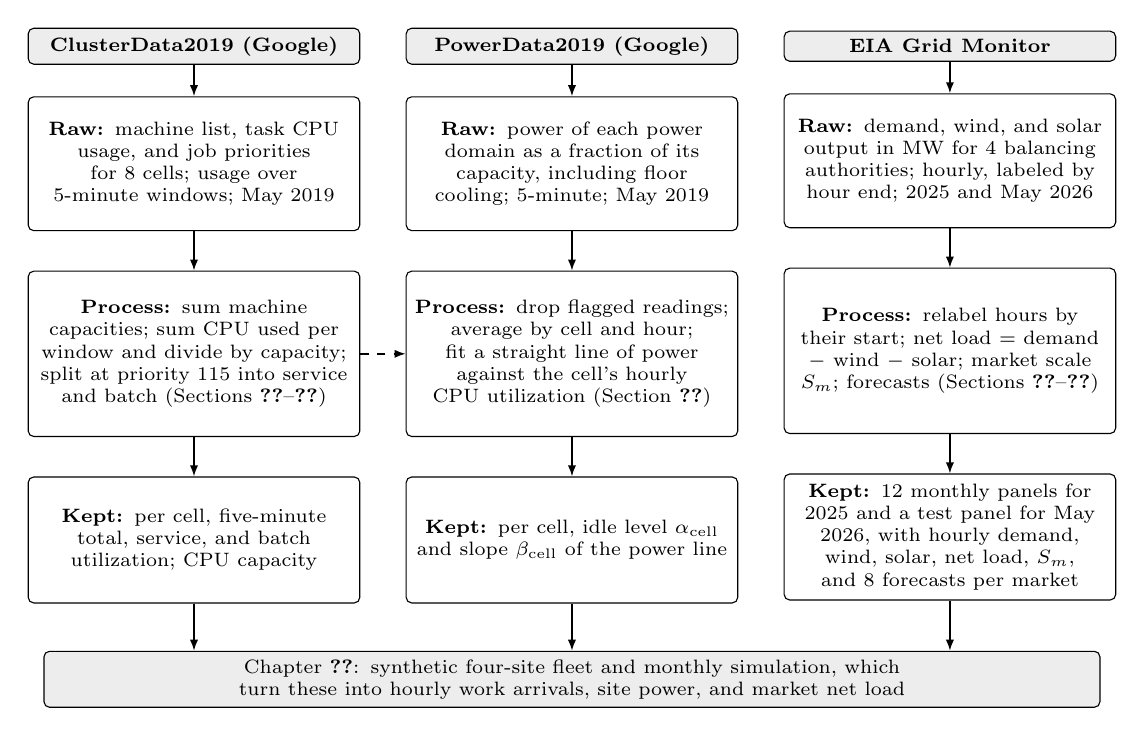
\begin{tikzpicture}[
    font=\scriptsize,
    box/.style={draw, rounded corners=2pt, align=center, inner sep=3pt,
      text width=40mm,
      execute at begin node={\hyphenpenalty=10000\exhyphenpenalty=10000}},
    head/.style={box, fill=black!7, font=\scriptsize\bfseries},
    arr/.style={-{Latex[length=1.4mm]}, semithick}
  ]
    \node[head] (h1) at (-4.8,0) {ClusterData2019 (Google)};
    \node[head] (h2) at (0,0) {PowerData2019 (Google)};
    \node[head] (h3) at (4.8,0) {EIA Grid Monitor};

    \node[box, below=4mm of h1, minimum height=17mm] (r1)
      {\textbf{Raw:} machine list, task CPU usage, and job priorities for
       8 cells; usage over 5-minute windows; May 2019};
    \node[box, below=4mm of h2, minimum height=17mm] (r2)
      {\textbf{Raw:} power of each power domain as a fraction of its
       capacity, including floor cooling; 5-minute; May 2019};
    \node[box, below=4mm of h3, minimum height=17mm] (r3)
      {\textbf{Raw:} demand, wind, and solar output in MW for 4 balancing
       authorities; hourly, labeled by hour end; 2025 and May 2026};

    \node[box, below=5mm of r1, minimum height=21mm] (p1)
      {\textbf{Process:} sum machine capacities; sum CPU used per window and
       divide by capacity; split at priority 115 into service and batch
       (Sections~\ref{sec:clusterdata2019}--\ref{subsec:clusterdata-tier-split})};
    \node[box, below=5mm of r2, minimum height=21mm] (p2)
      {\textbf{Process:} drop flagged readings; average by cell and hour; fit a
       straight line of power against the cell's hourly CPU utilization
       (Section~\ref{sec:powerdata2019})};
    \node[box, below=5mm of r3, minimum height=21mm] (p3)
      {\textbf{Process:} relabel hours by their start;
       net load \(=\) demand \(-\) wind \(-\) solar; market scale \(S_m\);
       forecasts
       (Sections~\ref{sec:energy-data}--\ref{subsec:energy-forecasts})};

    \node[box, below=5mm of p1, minimum height=16mm] (o1)
      {\textbf{Kept:} per cell, five-minute total, service, and batch
       utilization; CPU capacity};
    \node[box, below=5mm of p2, minimum height=16mm] (o2)
      {\textbf{Kept:} per cell, idle level \(\alpha_{\mathrm{cell}}\) and slope
       \(\beta_{\mathrm{cell}}\) of the power line};
    \node[box, below=5mm of p3, minimum height=16mm] (o3)
      {\textbf{Kept:} 12 monthly panels for 2025 and a test panel for May
       2026, with hourly demand, wind, solar, net load, \(S_m\), and 8
       forecasts per market};

    \node[box, fill=black!7, text width=132mm, below=6mm of o2] (sim)
      {Chapter~\ref{chap:problem}: synthetic four-site fleet and monthly
       simulation, which turn these into hourly work arrivals, site power,
       and market net load};

    \foreach \i in {1,2,3} {
      \draw[arr] (h\i) -- (r\i);
      \draw[arr] (r\i) -- (p\i);
      \draw[arr] (p\i) -- (o\i);
      \draw[arr] (o\i.south) -- (o\i.south |- sim.north);
    }
    \draw[arr, dashed] (p1) -- (p2);
  \end{tikzpicture}
  \caption[Data pipeline from the three public sources]{Data pipeline from the three public sources to the inputs of the
  simulation. The dashed arrow marks the hourly CPU utilization that the power
  fit uses.}
  \label{fig:data-pipeline}
\end{figure}

The raw data is large and detailed, and most of that detail is not needed.
The workload trace records every task on about 96,000 machines, but the
scheduler moves aggregate amounts of work, not individual jobs. The trace is
therefore reduced to how busy each cell is in each five-minute window, split
into work that must run at once (service) and work that may wait (batch).
The power trace is reduced to one straight line per cell that converts CPU
utilization into power. The grid data is kept hourly, as recorded, and gains
three derived quantities: net load, a fixed size scale for each market, and
forecasts of the coming hours.

The two Google traces cover May 2019, and the grid data covers 2025 and May
2026. They are merged in Chapter~\ref{chap:problem}, where the
744-hour workload of cells \(a\)--\(d\) is replayed in every month of 2025,
and that of cells \(e\)--\(h\) is replayed with the May 2026 grid data.

\section{Workload Data: Google ClusterData2019}
\label{sec:clusterdata2019}

\subsection{Dataset}
\label{subsec:clusterdata-role}

A \emph{Borg cell} is a group of machines managed as one computing cluster.
Google provides records for eight cells, labeled \(a\)--\(h\), from May 2019
\cite{wilkes2020clusterdata2019, tirmazi2020borg}. Two of Google's terms are
needed. A \emph{job} is a computation that a user wants to run, made up of one
or more \emph{tasks}, each a program running on one machine. An
\emph{allocation set} is a reservation of machine resources inside which a
job's tasks can run. Google's documentation calls jobs and allocation sets
\emph{collections}, and tasks and the reserved blocks \emph{instances}
\cite{wilkes2020clusterdata2019}. The trace records each machine's size, the
resources each task requested, the CPU each task used, and each job's
priority. It contains no user, application, or other identifying
information.

Three parts of the trace are used: the machine list, for each cell's CPU
capacity; the task usage measurements, for the CPU actually used; and the job
records, for priority. The trace is about 2.4 TiB compressed, too large to
download, so it is queried online through BigQuery, Google's cloud database
service.

Rather than tracking individual jobs and their execution, the aggregate CPU
utilization in each five-minute window is used as demand. This is how the
trace is summarized by Tirmazi \emph{et al.} in \emph{Borg: The Next
Generation} \cite{tirmazi2020borg}, who plot each priority tier's CPU usage as
a fraction of cell capacity over hour-long intervals, and by the utilization
code example in Google's GitHub repository, \emph{Google Trace Analysis Colab}
\cite{googleClusterAnalysisColab}.

\subsection{Fixed Reference Capacity}
\label{subsec:clusterdata-capacity}

Google measures CPU in Google compute units, an internal metric. The trace Google provides rescales them so that the largest
machine across all eight cells has a CPU capacity of 1.0, and every cell uses
this same scale \cite{wilkes2020clusterdata2019}. A machine with capacity 0.5
therefore has half the CPU of that largest machine. A cell's
\emph{reference capacity} \(C^{\mathrm{ref}}_{\mathrm{cell}}\) is the sum of these
capacities over its machines:
% [symbols 2026-10-09] was:
%   \sum_{n\in\mathcal{J}_c}\kappa_n ,
% where \(\mathcal{J}_c\), the \emph{machine set} of cell \(c\), is all
% machines ever observed in the cell, and \(\kappa_n\), the \emph{machine CPU
% capacity}, is machine \(n\)'s CPU capacity.
\begin{equation}
  C^{\mathrm{ref}}_{\mathrm{cell}}
  =
  \sum_{\text{machines in } cell}
  \bigl(\text{machine CPU capacity}\bigr),
  \label{eq:reference-capacity}
\end{equation}
where the sum covers every machine ever observed in the cell. A machine can appear in the
machine list several times during the month, for example when it is added,
removed, or changed, so its largest recorded capacity is used. Google's own
analysis notebook computes a cell's capacity the same way, by summing each
machine's largest recorded CPU capacity \cite{googleClusterAnalysisColab},
and divides hourly CPU use by it to plot usage as a fraction of cell
capacity, the measure reported by Tirmazi \emph{et al.} \cite{tirmazi2020borg}.
This gives a fixed monthly reference rather than the capacity active in each five-minute
interval, so the utilization defined next is measured relative to that fixed
reference.

Eight cells are captured in the trace. Cells \(a\)--\(d\) supply the training fleet, and
cells \(e\)--\(h\) supply the test fleet (Section~\ref{subsec:energy-calendar}).
Table~\ref{tab:cell-capacity} lists their reference capacities. Because every
cell uses the same scale, the sums can be compared across cells. One important note is that machine counts are a poor
guide to size: cell \(d\) has the second-largest number of machines among
\(a\)--\(d\) but the smallest capacity, because most of its machines are
small, and cell \(e\) has the most machines of all but less capacity than
\(f\), \(g\), or \(h\). 

\begin{table}[htbp]
  \centering
  \footnotesize
  \caption{Reference CPU capacity of the eight cells: \(a\)--\(d\) form the
  training fleet and \(e\)--\(h\) the test fleet.}
  \label{tab:cell-capacity}
  \begin{tabular}{@{}clrrr@{}}
    \toprule
    Cell & Fleet & Machines & \(C^{\mathrm{ref}}_{\mathrm{cell}}\) & Relative to cell \(c\) \\
    \midrule
    \(a\) & training & 10,001 & 6,835.7 & 0.897 \\
    \(b\) & training & 10,047 & 7,582.0 & 0.995 \\
    \(c\) & training & 13,245 & 7,619.8 & 1.000 \\
    \(d\) & training & 12,576 & 6,448.8 & 0.846 \\
    \addlinespace
    \(e\) & test & 14,122 & 7,266.9 & 0.954 \\
    \(f\) & test & 12,201 & 10,994.2 & 1.443 \\
    \(g\) & test & 12,796 & 7,963.1 & 1.045 \\
    \(h\) & test & 11,592 & 10,317.0 & 1.354 \\
    \bottomrule
  \end{tabular}
\end{table}

\subsection{Five-Minute Executed CPU}
\label{subsec:clusterdata-utilization}

For each five-minute window, the CPU used by all tasks is summed and divided
by the cell's fixed reference capacity. The result, the \emph{cell CPU
utilization} \(u_{\mathrm{cell},k}\), is the share of the cell's capacity in use in
window \(k\):
% [symbols 2026-10-09] was:
% utilization} \(u_{c,k}\), is the share of the cell's capacity in use. Let \(k\)
% identify the window and \(\mathcal{E}_{c,k}\), the window's \emph{measurement
% set}, denote its retained usage measurements:
%   \frac{\displaystyle\sum_{r\in\mathcal{E}_{c,k}} a_r}
% where \(a_r\), the \emph{measured CPU use}, is the average CPU used during
% measurement \(r\), on the same scale as machine capacity: a task that keeps a
\begin{equation}
  u_{\mathrm{cell},k}
  =
  \frac{\displaystyle\sum_{r\ \text{in window}\ k} a_r}
         {C^{\mathrm{ref}}_{\mathrm{cell}}} ,
  \label{eq:clusterdata-utilization}
\end{equation}
where \(k\) numbers the five-minute windows, and the sum runs over every
usage measurement \(r\) kept for window \(k\): one for each task or reserved
block running in it, after the two filters described below. The
\emph{measured CPU use} \(a_r\) is the average CPU used during
measurement \(r\), on the same scale as machine capacity: a task that keeps a
whole capacity-0.5 machine
busy for the full window has \(a_r=0.5\). The numerator and denominator are
on the same scale, so \(u_{\mathrm{cell},k}\) is a fraction of the cell's capacity.

Two kinds of usage measurements are left out. First, a task that runs inside
an allocation set draws its resources from a reserved block on its machine,
and Google reports the block's usage as the total for all the tasks running
inside it \cite{wilkes2020clusterdata2019}. Counting both the block and its
tasks would count the same CPU twice, so measurements of tasks inside a block
are dropped and the block's own measurement is kept. Second, Google reports
usage over measurement windows that are normally five minutes long but are
shorter when a task starts, stops, or changes during the window
\cite{wilkes2020clusterdata2019, googleTraceFormatV3}. Following the example
query in Google's analysis notebook \cite{googleClusterAnalysisColab}, only
measurements covering a full five minutes are kept, so each retained \(a_r\)
is an average over a whole window. An audit of cells \(a\)--\(d\) found that
dropping the shorter measurements only removes 6.5\% of CPU work.

\section{Service and Batch Classification}
\label{subsec:clusterdata-tier-split}

Google records job priorities rather than explicit service and batch
labels. The priority bands from Google's analysis in
Table~\ref{tab:priority-bands} are used. Work in the two lowest bands has weak
or no service-level objectives (SLOs), meaning it is assumed to be deferrable. Each usage measurement takes the
priority of its job, or of its allocation set for a reserved block.

\begin{table}[htbp]
  \centering
  \footnotesize
  \caption{ClusterData2019 priority bands used by the extraction.}
  \label{tab:priority-bands}
  \begin{tabular}{@{}llr@{}}
    \toprule
    Band & Interpretation in source & Priority \\
    \midrule
    Free & no-SLO & 0--99 \\
    Best-effort batch & no-SLO & 100--115 \\
    Mid & higher priority & 116--119 \\
    Production & higher priority & 120--359 \\
    Monitoring & higher priority & 360 and above \\
    \bottomrule
  \end{tabular}
\end{table}

% [symbols 2026-10-09] was:
% Priority 115 or below is classified as batch and the remaining usage as
% service. Let \(p_r\), the \emph{job priority}, be the priority of
% measurement \(r\)'s job, and \(\mathcal{E}^{\mathrm{bat}}_{c,k}\), the
% \emph{batch measurement set}, the measurements in \(\mathcal{E}_{c,k}\) with
% \(p_r\leq115\). Usage from a job with no recorded priority is counted as
% service.
%   \sum_{r\in\mathcal{E}^{\mathrm{bat}}_{c,k}} a_r,
Usage from jobs with priority 115 or below is classified as batch, and the
remaining usage as service. Usage from a job with no recorded priority is
counted as service. The two classes are the \emph{batch utilization}
\(u^{\mathrm{bat}}_{\mathrm{cell},k}\) and the \emph{service utilization}
\(u^{\mathrm{svc}}_{\mathrm{cell},k}\):
\begin{align}
  u^{\mathrm{bat}}_{\mathrm{cell},k}
  &=
  \frac{1}{C^{\mathrm{ref}}_{\mathrm{cell}}}
  \sum_{\substack{r\ \text{in window}\ k\\ \text{priority}\,\leq\,115}} a_r,
  \label{eq:batch-utilization}\\
  u^{\mathrm{svc}}_{\mathrm{cell},k}
  &=
  u_{\mathrm{cell},k}-u^{\mathrm{bat}}_{\mathrm{cell},k}.
  \label{eq:service-utilization}
\end{align}
These curves are referred to as \emph{deferrable batch} and
\emph{nondeferrable service}. Cells \(a\)--\(d\) supply the training
workload and cells \(e\)--\(h\) the test workload; both are converted to
hourly arrivals in Section~\ref{subsec:transform-pairing}. Appendix~\ref{app:data-schemas} lists the stored columns and example values.

Figure~\ref{fig:workload-week} shows the first week of the trace for the
four training cells, averaged by hour as the simulation uses it. Service
makes up most of each cell's load and follows a daily cycle, clearest in
cells \(a\) and \(d\); batch is a thinner band on top.

\begin{figure}[tbp]
  \centering
  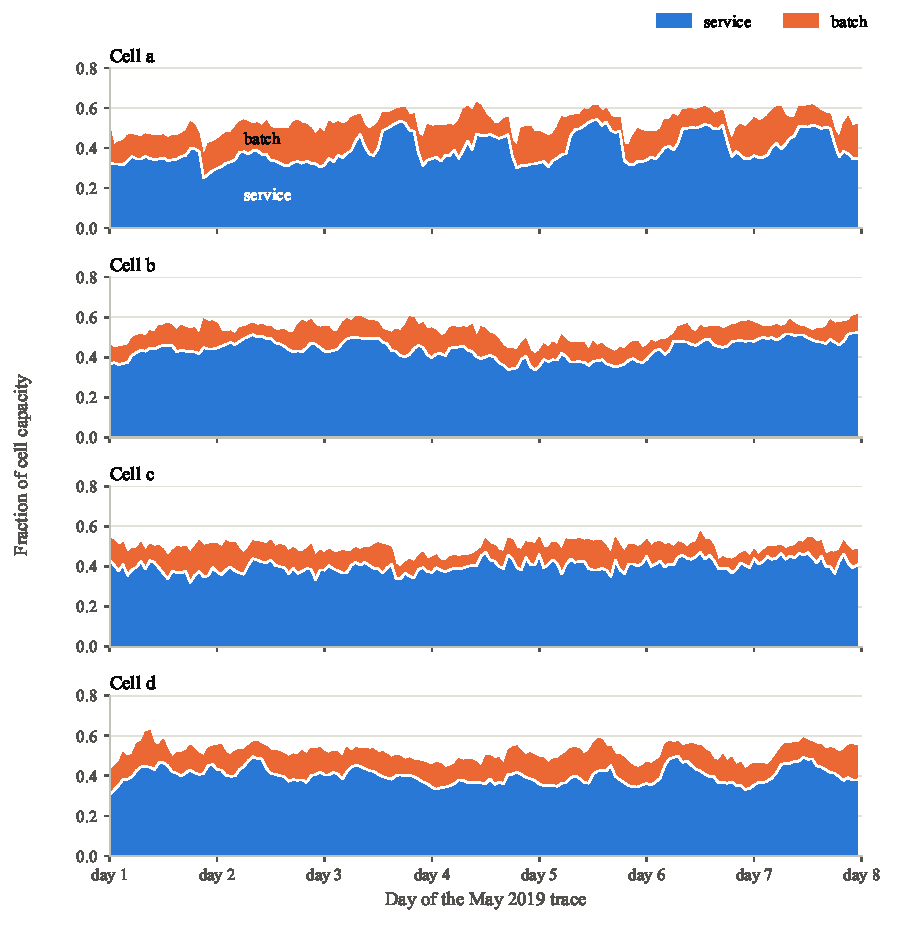
\includegraphics[width=\textwidth]{../docs/figures/data/workload_week.pdf}
  \caption[Hourly service and batch utilization of the training cells]{Hourly
  service and batch utilization of training cells \(a\)--\(d\) over the
  first week of the May 2019 trace, as a fraction of each cell's reference
  capacity.}
  \label{fig:workload-week}
\end{figure}

\section{Power Model: Google PowerData2019}
\label{sec:powerdata2019}

\subsection{Data Fit}
\label{subsec:powerdata-purpose}

PowerData2019 \cite{googlePowerData2019} provides five-minute power
measurements for the same Borg cells. Electricity reaches a data center's
machines through power distribution units, each feeding several rows of
server racks. Google calls the machines behind one such unit a
\emph{power domain}, and each cell has several. Every five minutes, the trace
reports each domain's power use as a fraction of what its unit can supply: a
value of 0.6 means the domain drew 60\% of its rated power. Power in MW is
not published. The measurements include data-center-floor cooling,
as stated on p.~2 of the \emph{Google Data Center Power Trace} documentation
\cite{googlePowerTraceDocumentation}. CPU utilization is used to predict this
measured power fraction; both series are averaged by cell and hour before an
ordinary least-squares line is fitted. The line gives the \emph{modeled power
fraction} \(\widehat p_{\mathrm{cell}}(u)\) of a cell at hourly CPU utilization \(u\):
\begin{equation}
  \widehat p_{\mathrm{cell}}(u)
  =
  \alpha_{\mathrm{cell}}+\beta_{\mathrm{cell}} u.
  \label{eq:powerdata-affine-fit}
\end{equation}
The intercept \(\alpha_{\mathrm{cell}}\), the \emph{idle power fraction}, is the modeled
power draw at zero CPU utilization, and the slope \(\beta_{\mathrm{cell}}\), the
\emph{dynamic power fraction}, is how much power rises from zero to full
utilization. The intercept
is an extrapolation: hourly CPU utilization ranges only from 0.35 to 0.68 in
the training cells and from 0.32 to 0.76 in the test cells, so the
least-squares line is extended beyond the observed data to reach zero. 

\subsection{Active Coefficients and Power Range}
\label{subsec:powerdata-coefficients}

Table~\ref{tab:powerdata-coefficients} lists the fitted coefficients for the
eight cells. Google reports power only as a fraction of capacity, so absolute
power must be assumed. The site built from the largest training cell, \(c\),
is assigned a reference power of 500 MW. Every other site's reference power,
in either fleet, is 500 MW multiplied by its cell's capacity relative to
\(c\) in Table~\ref{tab:cell-capacity}, which assumes that a cell's power
capacity is proportional to its CPU capacity. The reference powers then range
from 423 to 500 MW in the training fleet and from 477 to 721 MW in the test
fleet. 

\begin{table}[htbp]
  \centering
  \footnotesize
  \caption{Power fits using CPU utilization as the sole predictor, with
  power in MW at each site's reference power \(\overline P\). Cells
  \(a\)--\(d\) form the training fleet and \(e\)--\(h\) the test fleet.}
  \label{tab:powerdata-coefficients}
  \begin{tabular}{@{}crrrcrrrr@{}}
    \toprule
    Cell & \(\alpha_{\mathrm{cell}}\) & \(\beta_{\mathrm{cell}}\) & \(R^2\) & Observed \(u\)
         & \(\overline P\) & \(u=0\) & \(u=1\) & Swing \\
         & & & & & \multicolumn{4}{c}{MW} \\
    \midrule
    \(a\) & 0.528016 & 0.339728 & 0.7885 & 0.363--0.682
          & 449 & 237 & 389 & 152 \\
    \(b\) & 0.548190 & 0.375761 & 0.7479 & 0.415--0.654
          & 498 & 273 & 460 & 187 \\
    \(c\) & 0.439604 & 0.525740 & 0.7642 & 0.397--0.667
          & 500 & 220 & 483 & 263 \\
    \(d\) & 0.382039 & 0.570370 & 0.8005 & 0.346--0.627
          & 423 & 162 & 403 & 241 \\
    \addlinespace
    \(e\) & 0.388045 & 0.601116 & 0.9062 & 0.317--0.710
          & 477 & 185 & 472 & 287 \\
    \(f\) & 0.427230 & 0.440739 & 0.6472 & 0.405--0.700
          & 721 & 308 & 626 & 318 \\
    \(g\) & 0.456218 & 0.492296 & 0.7938 & 0.321--0.744
          & 523 & 238 & 496 & 257 \\
    \(h\) & 0.383827 & 0.392821 & 0.9432 & 0.318--0.763
          & 677 & 260 & 526 & 266 \\
    \bottomrule
  \end{tabular}
\end{table}



\section{Grid Data: EIA Demand, Wind, and Solar}
\label{sec:energy-data}

\subsection{Four Markets}
\label{subsec:energy-sources}

Each modeled site is assigned to an electricity market. Hourly demand and
generation by fuel are taken from the EIA grid monitor \cite{eiaGridMonitor}
for four balancing authorities, CAISO, MISO, SPP, and ISO-NE, each called a
\emph{market} in this thesis. Each series covers the whole balancing
authority.

For each market, demand, wind generation, and solar generation are used.
EIA labels each interval by its ending hour. One hour is subtracted so that
each hour is labeled by its beginning, in UTC, giving one record per market
per hour. The records for each month are stored in one table, called a
\emph{panel}; Appendix~\ref{app:data-schemas} lists its columns. For the test
month, the same three series are taken for May 2026, together with the week
before it and the first eighteen hours of June (UTC), which the forecasts need as
past inputs and as targets. 

\subsection{Net Load}
\label{subsec:energy-net-load}

Net load is demand minus wind and solar generation. Let \(\tau\) be a UTC
hour, \(D_m\) the \emph{gross demand} of market \(m\), and
\(G^{\mathrm{wnd}}_m\) and \(G^{\mathrm{sol}}_m\) its observed \emph{wind
output} and \emph{solar output}, all in MW. The \emph{net load} \(N_m\) is
\begin{equation}
  N_m(\tau)
  =
  D_m(\tau)
  -G^{\mathrm{wnd}}_m(\tau)
  -G^{\mathrm{sol}}_m(\tau).
  \label{eq:energy-net-load}
\end{equation}
Wind and solar output depends on the weather rather than the grid operator,
so it is taken as it comes; hydro and nuclear plants are not subtracted
because the operator schedules them. Net load is the demand left for those
scheduled sources to cover.

Figure~\ref{fig:net-load-week} shows one week of gross demand and net load
in each market, the week of the worked example in
Section~\ref{subsec:problem-worked-joint}. The gap between the two lines is
wind and solar output: wide in CAISO and SPP, and narrow in ISO-NE, where
net load nearly equals demand. CAISO's net load falls at midday as solar
output rises and climbs steeply in the evening.

\begin{figure}[tbp]
  \centering
  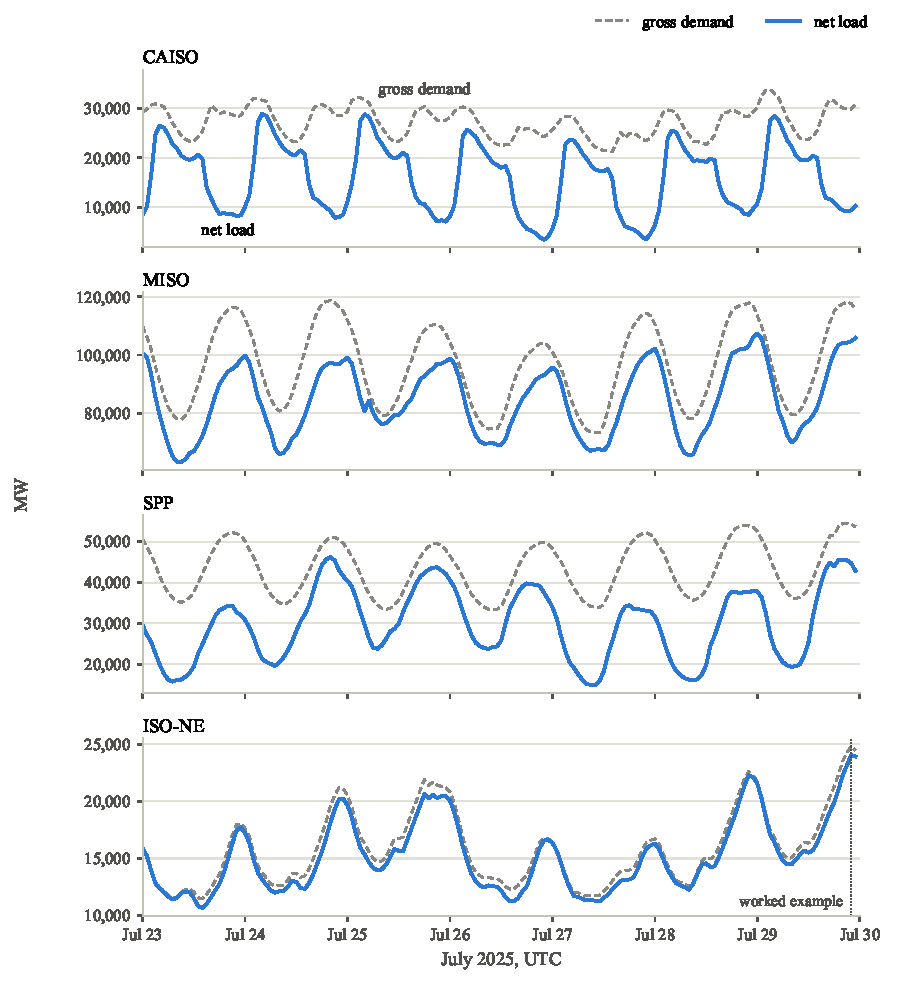
\includegraphics[width=\textwidth]{../docs/figures/data/net_load_week.pdf}
  \caption[One week of gross demand and net load in each market]{Hourly
  gross demand and net load of the four markets from 23 to 29 July 2025,
  UTC. The dotted line marks the hour of the worked example in
  Section~\ref{subsec:problem-worked-joint}.}
  \label{fig:net-load-week}
\end{figure}




% [dev-data 2026-10-10] was: \section{Development, Cross-Validation, and Test Data}
\section{Cross-Validation and Test Data}
\label{subsec:energy-calendar}

The data is divided by month, because each month is one
continuous simulation (Section~\ref{subsec:transform-pairing}) and the hours
within a month are linked: queued work carries from hour to hour, and every
ramp joins two neighboring hours. Two groups of months are used:
% [dev-data 2026-10-10] was: "Three groups of months are used:" and the bullets
%   \item The \emph{development data} is the twelve months of 2025, served by
%         the training fleet built from cells \(a\)--\(d\). Every design choice
%         and every fitted quantity comes from these months.
%   \item Within the development data, \emph{four-fold cross-validation}
%         estimates how well the method does on months it has not seen.
\begin{itemize}
  \item The \emph{training and validation data} is the twelve months of
        2025, served by the training fleet built from cells \(a\)--\(d\).
        Every design choice, and every value taken from the data, comes from
        these months. The scheduler is trained on them, and
        \emph{four-fold cross-validation} over them, the validation stage,
        estimates how well the method does on months it has not seen.
  \item The \emph{test data} is May 2026, served by a second fleet built
        from cells \(e\)--\(h\) (Section~\ref{subsec:transform-mapping}).
        May 2026 is used because it is the same calendar month as the Google
        trace, so the trace's 744 hours fill it exactly, and it lies a year
        after the 2025 data. The
        test month is scored only after every choice has been fixed.
\end{itemize}

In \(k\)-fold cross-validation, the data is divided into \(k\) equal parts,
called folds. A model is fitted on \(k-1\) folds and scored on the fold left
out, and this is repeated until every fold has been left out once; the \(k\)
scores are then averaged. Every
observation is scored exactly once, by a model that did not see it, so the
estimate does not depend on which part of the data happened to be held out,
as it would with a single validation month. Here \(k=4\), and each fold is
three whole months. 

Each fold uses one month from each third of the year, so its nine training
months include all four seasons, as the final training set does. Within a
fold, the forecast weights (Section~\ref{subsec:energy-forecasts}), the market
scales \(S_m\) below, and the objective references \(C_R\) and \(C_Q\)
(Section~\ref{subsec:problem-normalization}) all come from the fold's nine
training months only. The scheduler is then trained
on those nine months and scored on each of the three held-out months. With
three training runs per fold, every 2025 month is scored three times, each
time by a policy that never saw it, and the cross-validation estimate is the
average over the twelve months. After cross-validation, the final policies
are trained on all twelve months, with the same three quantities taken from
all twelve, and are then scored on the test month. No choice in the method is
made using the test month, so it stays a held-out test. 

\begin{table}[htbp]
  \centering
  \footnotesize
  \caption{Training and scored months of the four cross-validation folds and
  of the final policies. The 2025 months are served by the fleet from cells
  \(a\)--\(d\) and the test month by the fleet from cells \(e\)--\(h\).}
  \label{tab:data-splits}
  \begin{tabular}{@{}lll@{}}
    \toprule
    Stage & Training months & Scored months \\
    \midrule
    Fold 1 & the other nine months of 2025 & January, May, September 2025 \\
    Fold 2 & the other nine months of 2025 & February, June, October 2025 \\
    Fold 3 & the other nine months of 2025 & March, July, November 2025 \\
    Fold 4 & the other nine months of 2025 & April, August, December 2025 \\
    \addlinespace
    Final & all twelve months of 2025 & May 2026 (test) \\
    \bottomrule
  \end{tabular}
\end{table}

% [held-out 2026-10-10] was:
% Due to the forecasting input requirements, a training month that follows a held-out month starts from the last hour of
% that held-out month, and the forecasts for its first week use that month's
% observations as past inputs. These enter only as the starting point of the
% month's first ramp and as observations that were already available at the
% time. No held-out hour is ever scored during training, and the forecast
% weights leave out every row whose inputs reach into a held-out month
% (Section~\ref{subsec:energy-forecasts}).
In each fold, the held-out months sit between training months. For example,
fold 1 holds out May but trains on June. June can still look back into May:
its warm-up hour is the last hour of May, and its forecasts in the first week
use May's values as the yesterday and last week inputs.  What June cannot do is learn
from May. No May hour is scored during training, and no May hour is used to
fit the forecast model (Section~\ref{subsec:energy-forecasts}).

% [dev-data 2026-10-10] was: "differs from the development data" and "Every development month"
The test month differs from the 2025 months in three ways: its grid
data is a year later, its workload comes from cells \(e\)--\(h\) rather than
\(a\)--\(d\), and its fleet is larger, 2,398 MW against 1,869 MW
(Section~\ref{subsec:transform-mapping}). Every 2025 month replays the
same 744-hour workload of cells \(a\)--\(d\), so cross-validation scores new
grid months with familiar workload, while the test month also brings unseen
workload and an unseen fleet.

The training months of a split are written \(\mathcal E_{\mathrm{train}}\),
the \emph{training set}: nine months in a fold, and all twelve for the final
policies. To compare markets of different sizes, a fixed \emph{market scale}
\(S_m\) is defined for each market: the empirical 95th percentile of gross
demand over the training months,
% [symbols 2026-10-09] was:
%   Q_{0.95}\!\left(\{D_m(\tau):\tau\in\mathcal{R}\}\right),
% where \(\mathcal{R}\), the \emph{training hours}, is every hour of the
% training months.
\begin{equation}
  S_m
  =
  Q_{0.95}\!\left(\{D_m(\tau):\tau\ \text{in the training months}\}\right).
  \label{eq:market-scale}
\end{equation}
Each fold
computes its own scales from its nine months. The final scales in
Table~\ref{tab:frozen-stats} use all of 2025 and also serve the test month;
the fold scales lie within 4\% of them. The scales are held fixed throughout
training and evaluation and express net-load ramps and peaks relative to each
market's demand scale.
Using the 95th percentile rather than the highest hour keeps a few demand
spikes from dominating the scale. For example, ISO-NE's highest hour in 2025
reached 25,898~MW, 45\% above its 95th percentile, and only six hours of the
year came within 5\% of that peak. Scaling by that hour would make every
ISO-NE ramp and peak look about 30\% smaller.

\begin{table}[htbp]
  \centering
  \footnotesize
  \caption{Market scale \(S_m\), in MW: the final value from
  all of 2025, and the range of the four fold values.}
  \label{tab:frozen-stats}
  \begin{tabular}{@{}lrr@{}}
    \toprule
    Market & Final \(S_m\) & Fold range \\
    \midrule
    CAISO          & 33,781  & 32,499--34,530 \\
    MISO           & 100,521 & 97,645--102,611 \\
    SPP            & 45,876  & 44,457--47,237 \\
    ISO-NE         & 17,888  & 17,507--18,142 \\
    \bottomrule
  \end{tabular}
\end{table}

\section{Demand and Net-Load Forecasts}
\label{subsec:energy-forecasts}

Each hour of a panel is stored with gross-demand and net-load forecasts
issued at that hour, with lead times of one, three, six, and twelve hours.
The decision for hour \(t\) is made at the start of that hour, before its
demand and generation are known. Because each record is labeled by the hour
it begins (Section~\ref{subsec:energy-sources}), the latest complete record
at that moment is hour \(t-1\). The decision therefore reads the panel for
hour \(t-1\), so the forecasts available to it target \(t\), \(t+2\),
\(t+5\), and \(t+11\): the current decision hour and two, five, and eleven
hours later. The forecasts are produced from the EIA data by least-squares
regression.

\subsection{Forecast Model}
Each forecast is a linear regression: a constant plus a weighted sum of nine
inputs, all observed at or before the hour at which the forecast is issued.
Let the \emph{forecast quantity} \(Y\) stand for either gross demand \(D_m\)
or net load \(N_m\) of one market, let \(\tau\) be the \emph{issue hour},
\(\mathrm{hour}(\tau)\) its UTC \emph{hour of day} (0 to 23), and
\(h\in\{1,3,6,12\}\) the \emph{lead} in hours. The \emph{forecast}
\(\widehat Y(\tau+h\mid\tau)\) of \(Y\) at the \emph{target hour} \(\tau+h\)
is a constant \(b_0\) plus each \emph{forecast input} \(x_1,\dots,x_9\) times
its weight:
% [forecast-eq 2026-10-10] was the three-line form:
%   b_0
%   +b_1\,Y(\tau)
%   +b_2\,\bigl[Y(\tau)-Y(\tau-1)\bigr]
%   +b_3\,Y(\tau-24)
%   +b_4\,Y(\tau+h-24)
%   +b_5\,Y(\tau+h-168)
%   +b_6\sin\frac{2\pi\,\mathrm{hour}(\tau)}{24}
%   +b_7\cos\frac{2\pi\,\mathrm{hour}(\tau)}{24}
%   +b_8\,G^{\mathrm{wnd}}_m(\tau)
%   +b_9\,G^{\mathrm{sol}}_m(\tau).
\begin{equation}
  \widehat Y(\tau+h\mid\tau)
  =
  b_0+b_1x_1+b_2x_2+\dots+b_9x_9 .
  \label{eq:forecast-model}
\end{equation}
Table~\ref{tab:forecast-inputs} lists the nine inputs: five past values of
\(Y\), two terms for the time of day, and the wind and solar output at the
issue hour. 
% [forecast-eq 2026-10-10] was: "Table~\ref{tab:forecast-inputs} lists the nine
% inputs. Two of the lagged inputs look back ... The sine and cosine together ..."

\begin{table}[htbp]
  \centering
  \footnotesize
  % [forecast-eq 2026-10-10] added the first column (x_1 to x_9), the sine
  % and cosine formula, and split wind and solar into their own rows.
  \caption{Inputs \(x_1,\dots,x_9\) of the forecast model in
  Equation~\eqref{eq:forecast-model}. \(Y\) is the gross demand or the net
  load of one market, \(\tau\) is the issue hour, and \(h\) is the lead.}
  \label{tab:forecast-inputs}
  \begin{tabular}{@{}L{0.07\columnwidth}L{0.23\columnwidth}L{0.27\columnwidth}L{0.33\columnwidth}@{}}
    \toprule
    Input & Value & Meaning & Role \\
    \midrule
    \(x_1\) & \(Y(\tau)\)
      & latest value
      & starting point \\
    \addlinespace
    \(x_2\) & \(Y(\tau)-Y(\tau-1)\)
      & change over the last hour
      & how fast the series is already moving \\
    \addlinespace
    \(x_3\) & \(Y(\tau-24)\)
      & issue hour, one day earlier
      & with \(x_4\), yesterday's change from the issue hour to the
        target hour \\
    \addlinespace
    \(x_4\) & \(Y(\tau+h-24)\)
      & target hour, one day earlier
      & daily cycle \\
    \addlinespace
    \(x_5\) & \(Y(\tau+h-168)\)
      & target hour, one week earlier
      & weekly cycle, such as weekdays versus weekends \\
    \addlinespace
    \(x_6\), \(x_7\) & sine and cosine of \(2\pi\,\mathrm{hour}(\tau)/24\)
      & time of day of the issue hour
      & typical level for that time of day \\
    \addlinespace
    \(x_8\) & \(G^{\mathrm{wnd}}_m(\tau)\)
      & wind output at the issue hour
      & current weather \\
    \addlinespace
    \(x_9\) & \(G^{\mathrm{sol}}_m(\tau)\)
      & solar output at the issue hour
      & current weather \\
    \bottomrule
  \end{tabular}
\end{table}

The \emph{forecast weights} \(b_0,\dots,b_9\) are found by ordinary least
squares. A separate set of weights is fitted for
each market, quantity, and lead, so four markets, two quantities, and four
leads give 32 models. The weights differ by lead because a twelve-hour
forecast leans less on the latest value, and more on the value one week
earlier, than a one-hour forecast does. The simplest possible forecast,
\emph{persistence}, assumes that the value \(h\) hours ahead equals the latest
observed value. It is Equation~\eqref{eq:forecast-model} with \(b_1=1\) and
every other weight zero, and it is the benchmark the model must beat.

The model is static: its weights are fitted once, on the training months,
and then held fixed. They are not refitted as the simulation advances; each
hour, only the inputs change, as the newest observations enter
Equation~\eqref{eq:forecast-model}. A forecast for May 2026 therefore uses
weights learned from 2025 alone and values observed up to its issue hour.

\subsection{Fitting}
% [held-out 2026-10-10] was:
% The training data is the hourly EIA gross demand, net load, wind output,
% and solar output of each balancing authority over the training months. A
% fitting row pairs an issue hour with its target \(h\) hours later. A row is
% used only if its target hour, and every hour its inputs read, lie in training
% months. In a fold, this leaves out the rows whose target falls in a held-out
% month and the week of rows after each held-out month, whose week-ago input
% would otherwise read the held-out month; without this purge, a held-out
% month would shape the weights through the lagged inputs.
The forecast weights are fitted on the training months only. Each fitting
example, or \emph{row}, is one issue hour: its nine inputs and the value
that actually occurred \(h\) hours later. A row is used only if all of its
hours, inputs and target, fall in training months. Because one input looks
back a week, this removes the held-out months and the first week after each
held-out month. Forecasts are still made for those hours; their rows are
only left out of fitting the weights, so that the held-out months never
shape the forecast model.

Each model outputs a forecast in MW. For every hour, the eight forecasts of
each market are stored in the panel next to that hour's grid data
(Appendix~\ref{app:data-schemas}); each fold stores its own forecasts, and
the final models' forecasts fill the 2025 panels and the test panel. The
scheduler reads these stored forecasts as part of its observation and never
runs the model itself. 

\subsection{Accuracy}
% [mae-only 2026-10-10] was: "Three measures of forecast error are reported." with MAE,
% RMSE, and MAPE in one align block, plus a paragraph explaining RMSE and MAPE.
Forecast error is measured by the mean absolute error (MAE). For \(n\)
forecasts \(\widehat Y_i\) of realized values \(Y_i\),
\begin{equation}
  \mathrm{MAE}
  =
  \frac{1}{n}\sum_{i=1}^{n}\bigl|\widehat Y_i-Y_i\bigr|.
  \label{eq:forecast-metrics}
\end{equation}
The MAE is the typical size of a miss, in MW.
% [mae-only 2026-10-10] cut: "To compare markets of different size, it is also
% given as a share of the market scale \(S_m\)."

The MAE is computed on two sets of hours and compared with persistence.
The cross-validation set is every hour of 2025, each forecast by the fold
model that did not see its month. The test set is the 744 issue hours of May
2026, forecast by the final models. Table~\ref{tab:forecast-accuracy} reports
the MAE of both.

\begin{table}[htbp]
  \centering
  \footnotesize
  \caption{Forecast mean absolute error in MW, least-squares model (LS)
  versus persistence, by lead \(h\) in hours from the issue hour. The
  cross-validation rows pool every 2025 hour, each forecast by the fold model
  that held its month out; the test rows score May 2026 with the final
  models.}
  \label{tab:forecast-accuracy}
  \setlength{\tabcolsep}{4pt}
  \begin{tabular}{@{}llrrrrrrrr@{}}
    \toprule
    & & \multicolumn{2}{c}{\(h=1\)} & \multicolumn{2}{c}{\(h=3\)}
        & \multicolumn{2}{c}{\(h=6\)} & \multicolumn{2}{c}{\(h=12\)} \\
    \cmidrule(lr){3-4}\cmidrule(lr){5-6}\cmidrule(lr){7-8}\cmidrule(l){9-10}
    Market & Quantity & LS & Persist. & LS & Persist.
                & LS & Persist. & LS & Persist. \\
    \midrule
    \multicolumn{10}{@{}l}{\emph{Cross-validation, 2025}} \\
    CAISO          & gross demand &   387 &   863 &   728 & 2,234 &   938 & 3,437 & 1,043 &  3,546 \\
    CAISO          & net load     &   548 & 1,583 & 1,077 & 4,258 & 1,416 & 7,251 & 1,609 &  9,366 \\
    MISO           & gross demand &   452 & 1,745 & 1,231 & 4,968 & 1,987 & 8,626 & 2,628 & 10,961 \\
    MISO           & net load     &   876 & 2,034 & 2,393 & 5,405 & 3,789 & 8,544 & 4,952 &  9,981 \\
    SPP            & gross demand &   248 &   758 &   716 & 2,164 & 1,161 & 3,782 & 1,453 &  4,868 \\
    SPP            & net load     &   581 & 1,050 & 1,732 & 2,926 & 2,986 & 5,204 & 4,020 &  7,395 \\
    ISO-NE         & gross demand &   217 &   497 &   554 & 1,336 &   800 & 2,063 &   912 &  2,080 \\
    ISO-NE         & net load     &   232 &   525 &   604 & 1,406 &   869 & 2,156 &   984 &  2,151 \\
    \addlinespace
    \multicolumn{10}{@{}l}{\emph{Test, May 2026}} \\
    CAISO          & gross demand &   415 &   845 &   836 & 2,186 & 1,021 & 3,169 & 1,111 &  2,814 \\
    CAISO          & net load     &   532 & 1,524 &   993 & 4,141 & 1,250 & 7,226 & 1,395 & 10,693 \\
    MISO           & gross demand &   420 & 1,509 & 1,083 & 4,321 & 1,765 & 7,772 & 2,407 & 10,609 \\
    MISO           & net load     & 1,037 & 1,964 & 2,733 & 5,139 & 4,123 & 7,893 & 5,148 &  9,585 \\
    SPP            & gross demand &   226 &   791 &   661 & 2,301 & 1,036 & 4,188 & 1,393 &  5,781 \\
    SPP            & net load     &   558 & 1,011 & 1,561 & 2,804 & 2,595 & 5,033 & 4,001 &  7,303 \\
    ISO-NE         & gross demand &   236 &   419 &   586 & 1,109 &   783 & 1,721 &   849 &  1,872 \\
    ISO-NE         & net load     &   265 &   456 &   645 & 1,201 &   852 & 1,852 &   942 &  2,011 \\
    \bottomrule
  \end{tabular}
\end{table}

% [mae-only 2026-10-10] cut the RMSE and MAPE sentences, then (same day) the
% rest of the paragraph: MAE as 0.4-1.6% (h1) / 2.3-8.8% (h12) of S_m vs
% persistence 1.5-4.7% / 8.3-31.6%; training/CV error ratio 92-99% (no
% overfitting); test errors close to CV, so 2025 weights carry over to 2026.
Every model beats persistence at every lead on both sets, with a mean
absolute error 41\% to 87\% lower. The hourly grid panels contain demand, wind and solar generation, net load, the fixed market scale, and forecasts for each market. Appendix~\ref{app:data-schemas} lists the columns and an example row.

\section{Data Quality Checks}
\label{sec:data-quality}

% [data-quality 2026-10-10] replaced the \planned note (gap filling, hour shift,
% forecast causality checks).
No hour was missing in the EIA data for 2025 or the test month. Negative
wind or solar values are set to zero.

One implausible value is kept as EIA published it. CAISO's demand at
2025-07-31 20:00 UTC is 11,819 MW, against 29,881 and 29,886 MW in the hours
before and after, so its net load that hour is \(-7{,}242\) MW and two
artificial ramps of about 18,000 MW appear in July. Reviewing every market
and both years for one-hour spikes of this kind found no other.

\chapter{SYNTHETIC FLEET AND PROBLEM FORMULATION}
\label{chap:problem}

This chapter turns the prepared data into synthetic four-site fleets, one
for training and one for the test month, and states the optimization problem
the scheduler must solve. Nothing in it
depends on the learning method, so any scheduler can be scored against the
same problem.

\section{The Four-Site Fleet}
\label{sec:data-transformations}
\label{subsec:transform-mapping}

The study uses its own fixed cell-to-market mapping in
Table~\ref{tab:active-market-map}, which is an assumption rather than a
statement about where the cells are. The site index \(m\)
therefore identifies the source cell for its workload curves
\(u^{\mathrm{svc}}_{m,k},u^{\mathrm{bat}}_{m,k}\) and power coefficients
\(\alpha_m,\beta_m\). Each site also keeps the size of its source cell.
% [no-K 2026-10-10] was: compute capacity K_m = cell's reference capacity divided
% by that of cell c; reference power \overline P_m = 500 K_m MW.
Its capacity is the cell's reference capacity \(C^{\mathrm{ref}}_m\) from
Equation~\eqref{eq:reference-capacity}, and its \emph{reference power} is
\(\overline P_m=500\,C^{\mathrm{ref}}_m/7{,}619.8\) MW, where 7,619.8 is the
reference capacity of cell \(c\), the largest training cell; the site built
from cell \(c\) therefore has 500 MW (Table~\ref{tab:active-market-map}). The training fleet is built from
cells \(a\)--\(d\) and serves every 2025 month. The test fleet is built in the
same way from cells \(e\)--\(h\), placed in the same four markets in the same
order, and serves only the test month. Its sites are measured against the
same cell \(c\), so three of them exceed 500 MW, and the test fleet totals
2,398 MW against the training fleet's 1,869 MW.

\begin{table}[htbp]
  \centering
  \footnotesize
  \caption{Source cell and size of each modeled site, named by its market,
  for the training fleet and the test fleet.}
  \label{tab:active-market-map}
  % [no-K 2026-10-10] the K_m columns (0.897/0.995/1.000/0.846, total 3.738;
  % 0.954/1.443/1.045/1.354, total 4.796) became C^ref_m.
  \begin{tabular}{@{}lcrrcrr@{}}
    \toprule
    & \multicolumn{3}{c}{Training fleet} & \multicolumn{3}{c}{Test fleet} \\
    \cmidrule(lr){2-4}\cmidrule(l){5-7}
    Market & Cell & \(C^{\mathrm{ref}}_m\) & \(\overline P_m\) (MW)
                & Cell & \(C^{\mathrm{ref}}_m\) & \(\overline P_m\) (MW) \\
    \midrule
    CAISO          & \(a\) & 6,835.7 & 449 & \(e\) & 7,266.9 & 477 \\
    MISO           & \(b\) & 7,582.0 & 498 & \(f\) & 10,994.2 & 721 \\
    SPP            & \(c\) & 7,619.8 & 500 & \(g\) & 7,963.1 & 523 \\
    ISO-NE         & \(d\) & 6,448.8 & 423 & \(h\) & 10,317.0 & 677 \\
    \addlinespace
    Total          &       & 28,486.3 & 1,869 &     & 36,541.2 & 2,398 \\
    \bottomrule
  \end{tabular}
\end{table}

Decisions are hourly, and every work and power quantity below is for one
hour.
% [no-K 2026-10-10] was: a work unit = what the site built from cell c completes
% in one hour at full utilization; ISO-NE completes at most K_m = 0.846; one work
% unit adds 500 beta_m MW at any site m.
One \emph{work unit} uses the CPU scale of
Section~\ref{subsec:clusterdata-capacity}, on which
\(C^{\mathrm{ref}}_{\mathrm{cell}}\) is built: a work unit is the largest machine in
the trace running at full capacity for one hour. Each site carries this over
to its market: its capacity \(C^{\mathrm{ref}}_m\) is the
\(C^{\mathrm{ref}}_{\mathrm{cell}}\) of the cell placed in market \(m\), and
is the most work the site can complete in one hour. A work unit
is the same amount of computation at every site, so work from different
sites can be added and moved between them. A site's utilization is its work
divided by \(C^{\mathrm{ref}}_m\). Because the power coefficients
\(\alpha_m,\beta_m\) differ, the same work draws different power at each
site.

\section{Monthly Simulation and Hourly Arrivals}
\label{subsec:transform-pairing}

Simulated months follow the clock of the Google trace, which starts at
midnight Pacific daylight time on 1 May 2019, or 07:00 UTC. A fixed UTC\(-7\)
is used all year, so that each workload hour is replayed at the UTC hour
at which it was recorded: every month runs from 07:00 UTC on its first day
to 07:00 UTC on the first day of the next, and its first hour replays the
trace's first hour. Grid data stays in UTC; only the month boundaries
follow the trace. The 744-hour workload restarts at the beginning of each
month; shorter months use only the hours they need. The workload of cells
\(a\)--\(d\) is used in every 2025 month, whether a month is used for training
or held out in a fold, and the workload of cells \(e\)--\(h\) is used in the
test month.

Each month is an independent, continuous simulation. Queues and site-power
history carry across midnight, and every decision hour is scored. The
\emph{decision hours} for month \(e\) are \(\mathcal T_e=\{0,\ldots,T_e-1\}\),
where the \emph{month length} \(T_e\) is the month's number of hours.

% [symbols 2026-10-09] was: \(\mathcal W=\{-1\}\); for February 2025, ...
Each month's simulation starts one hour early, at the \emph{warm-up hour}
\(t=-1\); for February 2025, this is 06:00 UTC on 1~February. The
warm-up hour is not a decision hour and is never scored. It exists because
the month's first decision needs two things from the hour before it: the
grid data the scheduler observes for hour \(t-1\)
(Section~\ref{subsec:problem-causality}), and the site power from which the
month's first ramp, \(A_{m,0}-A_{m,-1}\), is measured
(Equation~\eqref{eq:adjusted-ramp}). Its grid data is what was recorded
for that hour, and its site power is what each site would have drawn running
that hour's arriving work in place. That work is not added to the queues, so
every month starts with empty queues, and the warm-up hour is left out of the
monthly peaks. Queues start empty and must be empty at month-end. 

Let the \emph{service arrivals} \(s_{m,t}\) and the \emph{batch arrivals}
\(q_{m,t}\) denote the hourly service and batch work arriving at site \(m\).
Service must run immediately; batch may wait.

The five-minute utilization curves from
Section~\ref{sec:clusterdata2019} are converted to work by averaging the
twelve windows in each hour, then multiplying by the site's capacity
\(C^{\mathrm{ref}}_m\). Multiplying by \(C^{\mathrm{ref}}_m\) is what lets work from different sites be
combined: a utilization is a fraction of one site's own capacity, and the
sites differ in size, so utilizations cannot be added across sites or moved
between them, while work units can. Each hour's recorded CPU execution is
treated as work
arriving at the start of the corresponding simulation hour, and the hour's
aggregate work is assumed known at that moment; for example, average
utilization of 60\% at the ISO-NE site becomes \(0.6\times6{,}448.8\approx3{,}869\) work
units. Let \(t\) be the hour within the month:
% [no-K 2026-10-10] was: K_m/12 in both arrival equations; examples 0.6 x 0.846 =
% 0.508, and 0.0897 + 0.0846 = 0.174 work units.
\begin{align}
  s_{m,t}
  &=
  C^{\mathrm{ref}}_m\,
  \frac{\displaystyle\sum_{b=0}^{11} u^{\mathrm{svc}}_{m,12t+b}}{12},
  \label{eq:synthetic-service-arrivals}\\[6pt]
  q_{m,t}
  &=
  C^{\mathrm{ref}}_m\,
  \frac{\displaystyle\sum_{b=0}^{11} u^{\mathrm{bat}}_{m,12t+b}}{12}.
  \label{eq:synthetic-batch-arrivals}
\end{align}
Each arrival is the site's average utilization over the hour's
twelve five-minute windows, times its capacity. Arrivals are
therefore amounts of work, not fractions of a site's capacity. If the CAISO
and ISO-NE sites are each 10\% utilized, they receive 683.6 and 644.9 work
units, 1,328.5 in total; moving all of it to the SPP site would make that site
17.4\% utilized. 

% [symbols 2026-10-09] was:
% Grid data from the corresponding UTC hours are used. If \(\tau_e\), the
% \emph{month start}, is the month's first UTC hour, the hourly demand
% \(D_{m,t}\) and net load \(N_{m,t}\) of decision hour \(t\), which falls
% \(t\) hours after the month start, are
% \begin{equation}
%   \begin{aligned}
%     D_{m,t} &= D_m(\tau_e+t), \\
%     N_{m,t} &= N_m(\tau_e+t).
%   \end{aligned}
%   \label{eq:episode-grid-map}
% \end{equation}
% This mapping also applies to the preceding warm-up hour.
% [no-D 2026-10-10] dropped D_{m,t}, which no equation uses.
Grid data comes from the matching UTC hours. The net load \(N_{m,t}\) of
decision hour \(t\) is the value of \(N_m\) recorded for the UTC hour \(t\)
hours after the month starts.

\section{Fleet Size Relative to Net-Load Ramps}
\label{subsec:transform-control-authority}

With the reference powers in Table~\ref{tab:active-market-map}, the sum of
the four individual idle-to-full modeled power ranges is approximately
844 MW for the training fleet, which can complete 28,486 work units per hour,
and 1,128 MW for the test fleet, which can complete 36,541.
% [no-K 2026-10-10] was: 3.738 and 4.796 work units per hour.
Table~\ref{tab:workload-feasibility} summarizes the repeated 744-hour
workloads. In the training fleet, median total arrivals use 55\% of capacity
and the largest hour uses 61\%; in the test fleet, they use 58\% and 68\%.

\begin{table}[htbp]
  \centering
  \footnotesize
  \caption{Fleet workload statistics in work units per hour.}
  \label{tab:workload-feasibility}
  \begin{tabular}{@{}lrrr@{}}
    \toprule
    Quantity & Median & Q95 & Maximum \\
    \midrule
    % [no-K 2026-10-10] values were in the old unit (cell c's hourly capacity):
    % training 1.614/1.843/1.958, 0.408/0.557/0.724, 2.054/2.210/2.269;
    % test 2.108/2.393/2.542, 0.669/0.899/1.033, 2.793/3.116/3.253.
    \multicolumn{4}{@{}l}{\emph{Training fleet, cells \(a\)--\(d\)}} \\
    Service arrivals & 12,301 & 14,045 & 14,916 \\
    Batch arrivals   & 3,107 & 4,243 & 5,520 \\
    Total arrivals   & 15,651 & 16,836 & 17,291 \\
    \addlinespace
    \multicolumn{4}{@{}l}{\emph{Test fleet, cells \(e\)--\(h\)}} \\
    Service arrivals & 16,063 & 18,236 & 19,371 \\
    Batch arrivals   & 5,099 & 6,849 & 7,873 \\
    Total arrivals   & 21,285 & 23,743 & 24,785 \\
    \bottomrule
  \end{tabular}
\end{table}

% [ramp-table 2026-10-10] was a paragraph comparing each site's idle-to-full
% range with the median and Q90 "original grid ramps" (training 17/11/34/55%,
% Q90 4-22%; test 32/19/33/61%); the numbers now sit in the table.
Table~\ref{tab:native-ramp-scale} compares each site's power swing, from
idle to full, with the hour-to-hour change in its market's net load over
2025. A training site's swing is about half of a typical change in ISO-NE
and a third in SPP, but only a tenth to a sixth in MISO and CAISO, so the
fleet has the most influence where hourly changes are small.

\begin{table}[htbp]
  \centering
  \footnotesize
  % [ramp-table 2026-10-10] dropped the Q90 column (4,270 / 4,316 / 2,423 / 1,089 MW).
  \caption{Median absolute hour-to-hour change in net load over 2025, and
  each site's power swing from idle to full
  (Table~\ref{tab:powerdata-coefficients}), in MW and as a share of that
  change.}
  \label{tab:native-ramp-scale}
  \begin{tabular}{@{}lrrrrr@{}}
    \toprule
    & & \multicolumn{2}{c}{Training site} & \multicolumn{2}{c}{Test site} \\
    \cmidrule(lr){3-4}\cmidrule(l){5-6}
    Market & Median absolute change & Swing & \% of median & Swing & \% of median \\
    \midrule
    CAISO          & 909   & 152 & 17 & 287 & 32 \\
    MISO           & 1,641 & 187 & 11 & 318 & 19 \\
    SPP            & 779   & 263 & 34 & 257 & 33 \\
    ISO-NE         & 435   & 241 & 55 & 266 & 61 \\
    \bottomrule
  \end{tabular}
\end{table}


\section{Decisions and Constraints}
\label{sec:problem-statement}

\subsection{Sets, Inputs, and Units}
\label{subsec:problem-given-inputs}

Let the \emph{site set} \(\mathcal M=\{1,\ldots,4\}\) be the modeled sites
and their paired markets. The \emph{origin} index \(i\) and the
\emph{destination} index \(j\) identify where batch work arrived and where it
executes. As in Section~\ref{subsec:transform-pairing}, the decision hours
\(\mathcal T_e=\{0,\ldots,T_e-1\}\) index simulated month \(e\), which has
\(T_e\) hours, and \(t=-1\) is the warm-up hour. Each interval
% [symbols 2026-10-09] was: \(T_e\) hours, and \(\mathcal W=\{-1\}\) is the warm-up hour.
is one hour. 

For each site and hour, the model uses the service arrivals \(s_{m,t}\) and
batch arrivals \(q_{m,t}\), the capacity \(C^{\mathrm{ref}}_m\), the reference power
\(\overline P_m\), the idle and dynamic power fractions \(\alpha_m,\beta_m\),
the completion window \(H\), the net load \(N_{m,t}\), and the market
scale \(S_m\), fitted on training months only. Every work quantity below, including
arrivals, executed work, and backlogs, is in work units
(Section~\ref{subsec:transform-mapping}), so it can be summed across sites.

Work can be divided among sites. Individual jobs, memory limits, machine
types, application dependencies, and scheduling within a site are not
modeled. 

\subsection{Scheduler Controls}
\label{subsec:problem-decisions}

Each hour, the scheduler chooses:
\begin{enumerate}
  \item the \emph{executed service} \(x^{\mathrm{svc}}_{j,t}\), service work
        executed at destination \(j\);
  \item the \emph{batch release} \(z_t\), the total queued batch work
        executed now; and
  \item the \emph{executed batch} \(x^{\mathrm{bat}}_{j,t}\), that batch
        total divided by destination.
\end{enumerate}

\subsection{Immediate Service}
\label{subsec:problem-service}

All service arrivals must execute in the same hour; the scheduler chooses
where:
\begin{equation}
  \sum_{j\in\mathcal M}x^{\mathrm{svc}}_{j,t}
  =
  \sum_{m\in\mathcal M}s_{m,t},
  \qquad
  x^{\mathrm{svc}}_{j,t}\geq0.
  \label{eq:service-conservation}
\end{equation}
Both sides are in work units, so the sum holds even though the sites differ
in size. For example, if one site has a capacity of 10,000 work units and
another 1,000, and both are 10\% utilized, they receive 1,000 and 100 work
units of service. Equation~\eqref{eq:service-conservation} then requires
1,100 work units of service to run somewhere in the fleet that hour, split
among the sites in any way that fits their capacity.
% [no-K 2026-10-10] replaced the example, which ended: one site ten times another's capacity,
% both 10% utilized, receive 1,000 and 100 work units; the equation requires
% 1,100 in total, "which the larger site alone can execute".


\subsection{Batch Queue and Deadlines}
\label{subsec:problem-batch}

The scheduler chooses how much batch work to execute and distributes it
among sites with available capacity. Its execution site determines its
power consumption. Let \(z_t\) be the batch release, the \emph{origin
release} \(y_{i,t}\) the work released from origin \(i\)'s backlog, and
\(x^{\mathrm{bat}}_{j,t}\) the executed batch at destination \(j\). Released
work executes within the same hour:
\begin{equation}
  z_t
  =
  \sum_{i\in\mathcal M}y_{i,t}
  =
  \sum_{j\in\mathcal M}x^{\mathrm{bat}}_{j,t},
  \qquad
  x^{\mathrm{bat}}_{j,t}\geq0.
  \label{eq:batch-total}
\end{equation}
Let the \emph{batch backlog} \(B_{i,t}\) be origin \(i\)'s queued batch work
before the current arrivals. The batch arrivals \(q_{i,t}\) of
Equation~\eqref{eq:synthetic-batch-arrivals}, written here with the origin
index \(i\), increase the backlog, and the origin release \(y_{i,t}\) reduces
it. Released work cannot exceed available work:
\begin{align}
  B_{i,t+1}
  &=
  B_{i,t}+q_{i,t}-y_{i,t},
  \label{eq:queue-balance}\\
  0
  &\leq y_{i,t}\leq B_{i,t}+q_{i,t}.
  \label{eq:queue-availability}
\end{align}
The \emph{completion window} \(H\) is the number of hourly slots in which a
batch arrival may run, counting its arrival slot. With \(H=24\), batch may
execute immediately or in the following 23 hourly slots, completing within
24 hours and by month-end. A 24-hour completion
window for flexible work is the convention of Google's carbon-aware system
\cite{radovanovic2021carbonaware} and of the batch model of Haghshenas
\emph{et al.} \cite{haghshenas2022infrastructure}. \(H\) is an assumption
rather than a measurement, because the trace records when work ran, not when
it was due.

An arrival in the \emph{arrival slot} \(\nu\) must therefore run by its
\emph{deadline slot}
\begin{equation}
  d_{\nu}
  =
  \min\{\nu+H-1,\;T_e-1\}.
  \label{eq:batch-deadline}
\end{equation}
Releases follow one global earliest-deadline-first queue. All queued batch
work, from every origin, waits in one list ordered by deadline slot. Each
hour, the batch release \(z_t\) is taken from the front of the list, the work
due soonest first, whichever site it came from; work with equal deadlines is
taken from the lowest-numbered origin first, then in order of arrival.
\emph{Global} means the four origins share one list rather than each keeping
its own. Releases are increased when necessary to leave enough capacity to
complete the remaining work on time. For each
origin, cumulative execution, summed over hours 0 to \(t\),
must cover all work due:
% [symbols 2026-10-09] was: summed over the hours \(\rho\) up to \(t\),
\begin{equation}
  \sum_{\rho=0}^{t}y_{i,\rho}
  \geq
  \sum_{\substack{\nu\in\mathcal T_e\\d_{\nu}\leq t}}q_{i,\nu},
  \qquad i\in\mathcal M,\ t\in\mathcal T_e.
  \label{eq:deadline-feasibility}
\end{equation}
In words: by the end of hour \(t\), origin \(i\) must have released at least
as much work as all of its arrivals that are due by \(t\). With \(H=24\), for
example, an arrival in hour 7 may run in any of hours 7 to 30, so by the end
of hour 30 every batch arrival from hours 0 to 7 (deadline slots 23 to 30)
must have run. Because each origin's work is released in deadline
order, which within one origin is also arrival order, releasing that much
means every due arrival has run, not just the same amount of other work.
% [review 2026-10-10] dropped the terminal-queue equation B_{i,T_e} = 0
% (eq:terminal-queue); it follows from the equation above at t = T_e - 1.
Because every deadline is capped at the month's last hour, this rule at
\(t=T_e-1\) already requires every backlog to be empty when the month
ends.

\subsection{Capacity and Site Power}
\label{subsec:problem-feasibility}

Service and batch execution together, the \emph{executed work}
\(w_{m,t}\), cannot exceed the site's hourly capacity:
\begin{align}
  w_{m,t}
  &=
  x^{\mathrm{svc}}_{m,t}
  +x^{\mathrm{bat}}_{m,t},
  \label{eq:executed-work}\\
  0
  &\leq w_{m,t}\leq C^{\mathrm{ref}}_m.
  \label{eq:site-capacity}
\end{align}
% [no-K 2026-10-10] was: w <= K_m; reference power 500 K_m MW; ratio w/K_m.
Executed work is converted to power using the model from
Section~\ref{sec:powerdata2019} and the site's reference power
\(\overline P_m\) (Section~\ref{subsec:transform-mapping}). The ratio \(w_{m,t}/C^{\mathrm{ref}}_m\) is the
site's utilization, the quantity on which the fit in
Equation~\eqref{eq:powerdata-affine-fit} was estimated, and the \emph{site
power} \(P_{m,t}\) is
\begin{equation}
  P_{m,t}
  =
  \overline P_m
  \left(
    \alpha_m+\beta_m\frac{w_{m,t}}{C^{\mathrm{ref}}_m}
  \right)
  \quad\mathrm{MW}.
  \label{eq:runtime-power}
\end{equation}

Work may execute at any site with available capacity. Transfers have no
modeled latency, bandwidth limit, data-residency restriction, energy cost,
or movement charge. This gives the model an optimistic upper bound on
geographic flexibility.

\section{Net-Load Ramps and Peaks with the Fleet}
\label{subsec:problem-objective}

% [two-goals 2026-10-10] added the opening sentence and "For the first goal,"
% so that "The second goal" below has something to refer to.
The scheduler has two goals: to make each market's hourly net load ramps smaller, and to lower each market's highest net
load of the month. Both are measured on each market's net load after adding
modeled site power, the \emph{adjusted net load} \(A_{m,t}\):
\begin{equation}
  A_{m,t}
  =
  N_{m,t}+P_{m,t}.
  \label{eq:adjusted-net-load}
\end{equation}
For the first goal, changes in net load between consecutive hours are measured, before and after
adding fleet power. This one-hour interval matches the data and scheduling
decisions. Dividing by \(S_m\) expresses each one-hour change as a fraction
of the market's demand scale per hour, giving the \emph{original ramp}
\(\Delta^{\mathrm{original}}_{m,t}\) of the grid alone and the \emph{adjusted
ramp} \(\Delta^{\mathrm{adjusted}}_{m,t}\) with the fleet:
\begin{align}
  \Delta^{\mathrm{original}}_{m,t}
  &=
  \frac{N_{m,t}-N_{m,t-1}}{S_m},
  \label{eq:native-ramp}\\
  \Delta^{\mathrm{adjusted}}_{m,t}
  &=
  \frac{A_{m,t}-A_{m,t-1}}{S_m}.
  \label{eq:adjusted-ramp}
\end{align}
Squaring penalizes larger ramps and treats upward and downward ramps
equally. The fleet's \emph{ramp impact} \(I_{m,t}\) is measured by
subtracting the original grid's squared ramp:
\begin{equation}
  I_{m,t}
  =
  \left(\Delta^{\mathrm{adjusted}}_{m,t}\right)^2
  -
  \left(\Delta^{\mathrm{original}}_{m,t}\right)^2.
  \label{eq:incremental-impact}
\end{equation}
A negative value means the scheduled fleet reduced the squared ramp relative
to the original grid; a positive value means it increased it.

% [peaks 2026-10-10] was: separate equations for the adjusted peak
% Q^adjusted_{m,e}(mu) = max_t A_{m,t}(mu)/S_m (eq:monthly-peak) and the original
% peak Q^original_{m,e} = max_t N_{m,t}/S_m (eq:monthly-original-peak), then
% Phi = Q^adjusted - Q^original.
The second goal is to lower each market's highest net load of the month. A
\emph{scheduling policy} \(\mu\) is a rule that chooses every hour's
controls. As with ramps, the fleet's effect is measured against the grid
alone. The fleet's \emph{peak impact} \(\Phi_{m,e}(\mu)\) in month \(e\) is
the month's highest adjusted net load under policy \(\mu\), the
\emph{adjusted peak}, minus its highest original net load, the
\emph{original peak}, divided by \(S_m\):
\begin{equation}
  \Phi_{m,e}(\mu)
  =
  \frac{\displaystyle\max_{t\in\mathcal T_e} A_{m,t}(\mu)
        -\max_{t\in\mathcal T_e} N_{m,t}}{S_m}.
  \label{eq:peak-impact}
\end{equation}
No schedule can change the original peak, so subtracting it changes every
schedule's score by the same amount. It keeps the grid's own peak records,
which the scheduler cannot influence, out of the hourly training signal.
Site power is positive, so \(\Phi_{m,e}(\mu)>0\).

\section{Joint Objective}
\label{subsec:problem-normalization}

Ramp impact and monthly peaks have different numerical scales. To combine
them in one objective, each is divided by a fixed positive reference value.
The \emph{no-flexibility baseline} policy,
\(\mu_{\mathrm{NF}}\), runs all work immediately at its original site.
Using this policy over the training set \(\mathcal E_{\mathrm{train}}\), the
\emph{ramp reference} \(C_R\) and the \emph{peak reference} \(C_Q\) are
calculated as
\begin{align}
  C_R
  &=
  \frac{1}{|\mathcal E_{\mathrm{train}}|}
  \sum_{e\in\mathcal E_{\mathrm{train}}}
  \sum_{t\in\mathcal T_e}\sum_{m\in\mathcal M}
  \left(\Delta^{\mathrm{adjusted}}_{m,t}(\mu_{\mathrm{NF}})\right)^2,
  \label{eq:ramp-reference}\\
  C_Q
  &=
  \frac{1}{|\mathcal E_{\mathrm{train}}|}
  \sum_{e\in\mathcal E_{\mathrm{train}}}\sum_{m\in\mathcal M}
  \max_{t\in\mathcal T_e}\frac{A_{m,t}(\mu_{\mathrm{NF}})}{S_m}.
  % [peaks 2026-10-10] was: Q^{\mathrm{adjusted}}_{m,e}(\mu_{\mathrm{NF}})
  \label{eq:peak-reference}
\end{align}
Both references are totals for the whole grid with the no-flexibility fleet:
\(C_R\) is its average monthly total of squared ramps, and \(C_Q\) is its
average monthly sum of the markets' normalized peaks. Dividing by them expresses
a change in \(\sum_{t,m}I_{m,t}\) or \(\sum_m\Phi_{m,e}\) as a fraction of total
squared ramp or of total peak, so the equal weights below value equal
fractional reductions of the two totals.  After cross-validation, the final references are computed from all twelve months of 2025: \(C_R=6.102\) and
\(C_Q=3.653\). They also score the test month, which is never used to set
them. 

Each simulated month \(e\) is one optimization episode. Decisions are hourly,
and the objective covers the full month. The goal is to find the schedule
with the smallest equally weighted combination of scaled monthly ramp impact
and monthly peak impact. That combination is the \emph{joint
score} \(J_e(\mu)\). Let the \emph{feasible policy set} \(\mathfrak M\) be the
causal scheduling policies satisfying
Equations~\eqref{eq:service-conservation}--\eqref{eq:site-capacity}:
\begin{equation}
  \begin{aligned}
    &\min_{\mu\in\mathfrak M} J_e(\mu),\\
    &J_e(\mu)
    =
    \frac{0.5}{C_R}
    \sum_{t\in\mathcal T_e}\sum_{m\in\mathcal M} I_{m,t}(\mu)\\
    &\hspace{2em}
    +\frac{0.5}{C_Q}
    \sum_{m\in\mathcal M} \Phi_{m,e}(\mu).
  \end{aligned}
  \label{eq:objective}
\end{equation}
The 0.5 weights apply after dividing each term by its reference scale.
A lower joint score need not improve both components.

\section{Information Available to the Scheduler}
\label{subsec:problem-causality}

The scheduler chooses an action before the hour-\(t\) net load is revealed.
Once the hour ends, the action is scored using that realized net load.
% [symbols 2026-10-09] was: Its available information, the \emph{information set}
% \(\mathcal I_t\), consists of:
At decision hour \(t\), the scheduler can see only the following:
\begin{itemize}
  \item gross demand and net load for hour \(t-1\);
  \item the gross-demand and net-load forecasts issued at hour \(t-1\),
        which target \(t\), \(t+2\), \(t+5\), and \(t+11\) (the current
        decision hour and two, five, and eleven hours later);
  \item the hour-\(t\) service and batch arrivals, and each site's queued
        batch work;
  \item the \emph{urgency} of the queued batch work: how much of it must run
        within the next 1, 3, 6, 12, and 24 hours;
  \item modeled site power from hour \(t-1\);
  \item each market's running adjusted and original net-load peaks over
        completed decision hours (zero before the first decision); and
  \item UTC hour, UTC day of week, and the number of hours left in the
        month.
\end{itemize}

% [symbols 2026-10-09] was: ... must use only \(\mathcal I_t\).
Each decision under policy \(\mu\) may use only this information. Chapter~\ref{chap:method} describes the observation features and
the solution algorithm.

\section{Baseline and Formal Problem Statement}
\label{subsec:problem-evaluation}

The scheduler is compared with \(\mu_{\mathrm{NF}}\) using
the same arrivals, power models, grid data, forecasts, and month. Improvement
is reported as
\begin{equation}
  \text{Improvement}
  =
  J_e(\mu_{\mathrm{NF}})-J_e(\mu),
  \label{eq:improvement}
\end{equation}
which is positive when the scheduler \(\mu\) improves on the baseline.

The ramp-impact and peak components are reported separately, along with
each market's adjusted peak in MW and its reduction from
the no-flexibility fleet. Since site power is nonnegative, peak reduction
means improvement over that fleet without flexibility, not a peak below the
original grid without the fleet.

The full problem can now be stated.
\label{subsec:problem-formal-statement}

\begin{quote}
Choose a causal policy for hourly service destinations, batch release
volumes, and batch destinations to minimize the joint monthly ramp-impact and
net-load peak score in Equation~\eqref{eq:objective}. Use only the
information available at each decision and meet the service, deadline, and
capacity constraints above. Report improvement over the no-flexibility
baseline using Equation~\eqref{eq:improvement}.
\end{quote}


\section{Worked Example: Joint Ramp and Peak Reduction}
\label{subsec:problem-worked-joint}

An hour from July 2025 is selected to illustrate the joint
objective. This is a worked calculation, not a PPO result. The
no-flexibility baseline is compared with a schedule that changes one hour's
service routing and leaves all other work in place.

% [no-K 2026-10-10] was: 0.3003 service, 0.1733 batch, w = 0.4736, utilization
% 0.4736/0.8463, CAISO spare 0.4306 (old unit = cell c's hourly capacity).
At 2025-07-29 22:00 UTC (hour \(t=687\)), ISO-NE receives 2,528.1 work
units of service and 963.3 of batch. Under the baseline, it executes
\(w=3{,}491.5\) work units, a utilization of \(3{,}491.5/6{,}448.8=0.5414\), drawing
approximately
\begin{equation*}
  P = 423.16\,(0.382039 + 0.570370 \times 0.5414)
  \approx 292.3\ \mathrm{MW}.
\end{equation*}
CAISO draws 330.2 MW and has 2,648.3 work units of spare capacity.
Moving ISO-NE's 2,528.1 service work units to CAISO fits within that capacity.
ISO-NE's power falls to 197.7 MW, and CAISO's rises to 386.5 MW. Batch work
still runs at its original sites in its arrival hour.

Table~\ref{tab:joint-example-hour} shows the two markets' grid conditions
and the fleet's ramp impact. Routing changes ISO-NE's impact from positive
to negative, while CAISO's goes from about zero to slightly positive.
The 21:00 forecasts available at this decision
predicted current-hour net loads of 23,894 MW for ISO-NE and
9,135 MW for CAISO; scoring uses the realized net load.

\begin{table}[htbp]
  \centering
  \footnotesize
  \caption{Grid conditions and routing effects at 2025-07-29 22:00 UTC.
  Ramp impacts use Equation~\eqref{eq:incremental-impact}.}
  \label{tab:joint-example-hour}
  \begin{tabular}{@{}lrr@{}}
    \toprule
    Quantity & ISO-NE      & CAISO \\
    \midrule
    Original net load at 21:00 (MW) & 23,204 & 9,153 \\
    Original net load at 22:00 (MW) & 24,082 & 9,390 \\
    Ramp impact \(I_{m,t}\), baseline & \(+0.000034\) & \(-0.0000002\) \\
    Ramp impact \(I_{m,t}\), with routing & \(-0.000461\) & \(+0.000026\) \\
    \bottomrule
  \end{tabular}
\end{table}

ISO-NE's peak shows the effect most clearly. This hour sets the market's monthly adjusted
net-load peak under the baseline: \(24{,}082+292.34=24{,}374.34\) MW.
After routing, its peak is \(24{,}082+197.72=24{,}279.72\) MW, a reduction
of 94.62 MW. Checking every July hour confirms that no other hour exceeds
this new peak. CAISO's monthly peak remains 33,829.1 MW, and the MISO and
SPP peaks are unchanged.

Both schedules are calculated over all 744 hours, including the next-hour
ramp when service returns to its original sites.
Table~\ref{tab:joint-example-month} shows how the routing choice changes
the normalized monthly components. The joint score is their equally
weighted mean; calculations use unrounded inputs.

\begin{table}[htbp]
  \centering
  \footnotesize
  \caption{July scores for the illustrative routing change. All other work
  follows the no-flexibility baseline.}
  \label{tab:joint-example-month}
  \begin{tabular}{@{}lrr@{}}
    \toprule
    Quantity & Baseline & With routing \\
    \midrule
    ISO-NE monthly peak (MW) & 24,374.3 & 24,279.7 \\
    CAISO monthly peak (MW) & 33,829.1 & 33,829.1 \\
    Scaled ramp impact & \(-0.000178\) & \(-0.000279\) \\
    Scaled peak impact & 0.010367 & 0.008919 \\
    Joint score \(J_e\) & 0.005094 & 0.004320 \\
    \bottomrule
  \end{tabular}
\end{table}

The scaled peak impact is \(\sum_m\Phi_{m,e}/C_Q\), using July's original
peaks, including 24,082 MW for ISO-NE, and the final references \(C_R\) and
\(C_Q\). The joint improvement is about 0.00077, most of it from the lower
ISO-NE peak.
This one-hour routing change reduces both monthly scores while executing
the same work within the service, deadline, and capacity constraints.

% [merge 2026-10-21] Chapters 5 and 6, the comparison-run and limitation
% paragraphs, Appendix B's last three sections, and Appendices C and D come
% from latex/ppo_solution.tex, which this merge replaces.
\chapter{SCHEDULING METHOD: PROXIMAL POLICY OPTIMIZATION}
\label{chap:method}

% [review 2026-10-21] was three paragraphs: the research question and the
% three controls again; related work (Carbon-Aware Computing, DeepEE,
% SustainDC), parked in Chapter 2; and the three evaluation stages, which
% Section 3.6 already gives (their two new sentences moved to Section 5.7).
This chapter turns the problem of Chapter~\ref{chap:problem} into a
reinforcement-learning task, then describes how PPO trains the scheduler and
how the trained policies are scored.

\section{Reinforcement Learning Overview}
\label{sec:method-rl}

% [rl-overview 2026-10-22] replaced the planned note; was: "One interaction is
% one decision hour. The scheduler observes the available grid information and
% workload, chooses an action, and receives a reward once the hour's realized
% net load is known. One episode is one simulated month (Section 4.2)."
% [rl-overview 2026-10-22, later] user cut the opening definition, the
% forecast comparison, the Vazquez-Canteli/Kahil sentence, and the
% state-versus-observation paragraph; the discounting sentence was dropped.
Sutton and Barto, in \emph{Reinforcement Learning: An
Introduction}, describe \emph{reinforcement learning} as learning how to map
situations to actions so as to maximize a numerical reward, where the learner is not told which action is
correct and must find out by trying actions
\cite[Sec.~1.1]{sutton2018reinforcement}. Here it is used to find a scheduling rule
for the problem of Chapter~\ref{chap:problem}: a rule that acts each hour using only
the information available at that hour (Section~\ref{subsec:problem-causality}),
never the future, as a scheduler running in real time would have to. 

Sutton and Barto name two features that define reinforcement learning:
learning by trial and error, and delayed reward, because an action affects
not only the reward that follows it but also the situations and rewards after
it \cite[Sec.~1.1]{sutton2018reinforcement}. 

Reinforcement learning uses an \emph{agent}, the learner and
decision maker, that interacts with an \emph{environment}, everything outside
the agent, over a sequence of time steps. At each step the agent chooses an
\emph{action}, and the environment responds with a new situation and a
numerical \emph{reward} \cite[Sec.~3.1]{sutton2018reinforcement}.
Table~\ref{tab:rl-terms} gives the meaning of each term in this thesis. Anything
the agent cannot change arbitrarily belongs to the environment, so the
decoder that enforces the constraints and the calculation of the reward are
both part of the environment here
\cite[Sec.~3.1]{sutton2018reinforcement}.

\begin{table}[htbp]
  \centering
  \footnotesize
  \caption[Reinforcement-learning terms and their meaning in this thesis]{Reinforcement-learning
  terms \cite[Secs.~3.1--3.5]{sutton2018reinforcement} and their meaning in
  this thesis.}
  \label{tab:rl-terms}
  \begin{tabular}{@{}L{0.13\textwidth}L{0.30\textwidth}L{0.36\textwidth}L{0.11\textwidth}@{}}
    \toprule
    Term & General meaning & In this thesis & Section \\
    \midrule
    Agent & the learner and decision maker & the scheduler
      & \ref{sec:method-ppo} \\
    Environment & everything outside the agent
      & the monthly simulation of the fleet and the four markets, including
        the decoder & Ch.~\ref{chap:problem} \\
    Time step & one decision & one hour & \ref{subsec:transform-pairing} \\
    Observation & what the agent sees before it acts
      & 82 numbers built from the information of
        Section~\ref{subsec:problem-causality} & \ref{sec:method-observation} \\
    Action & the agent's choice
      & nine preferences, which the decoder turns into a feasible schedule
      & \ref{sec:method-actions} \\
    Reward & a number returned after each action
      & the hour's share of \(-J_e\) & \ref{sec:method-reward} \\
    Episode & the steps from a start to an end
      & one month, 672 to 744 hours & \ref{subsec:transform-pairing} \\
    Return & the sum of an episode's rewards
      & \(-J_e\) of the month & \ref{sec:method-reward} \\
    Policy & the rule that chooses actions
      & a small neural network, trained by PPO & \ref{sec:method-ppo} \\
    \bottomrule
  \end{tabular}
\end{table}

One hour of a simulated month shows how the terms fit together. The
scheduler, as the agent, reads the observation: the grid data of the
previous hour, the forecasts issued then, the hour's arrivals and queues, and
the other entries of Section~\ref{sec:method-observation}. It then chooses an
action. The environment turns the action into a schedule that meets every
constraint, computes each site's power, reveals the hour's net load, and
returns the hour's reward. The next hour starts from the queues and site
power that this hour left behind. After the month's last hour, the episode
ends with every queue empty, and the rewards of all its hours add up to the
month's \emph{return}, the joint score with its sign reversed, \(-J_e\). A schedule with a lower joint score therefore earns a higher return.

A \emph{policy} is a mapping from what the agent sees to the probabilities of
choosing each action, and a reinforcement-learning method specifies how the
policy changes with experience \cite[Sec.~3.5]{sutton2018reinforcement}. Here
the policy is a small neural network, and PPO is the method that changes it
(Sections~\ref{sec:method-ppo} and~\ref{sec:method-training}). The policy changes only during training, on the
training months. Once training ends, it is fixed and is scored on months it
never trained on (Section~\ref{sec:method-evaluation}).

\section{Observation}
\label{sec:method-observation}

% [review 2026-10-21] was a paragraph repeating the list of
% Section 4.7, and "Current arrivals are known when scheduling; realized grid
% measurements are available only through t-1."
% [obs-table 2026-10-22] the bullet list became Table 5.2, the scaling of each
% entry moved here from Section 5.5.3, and the climb paragraph was reworded;
% was: "The steepest forecast climb is the largest per-hour rise, as a share of
% S_m, along the path from the last observed value through the four forecasts;
% it is the only entry that Section 4.7 does not list."
The observation is the information of Section~\ref{subsec:problem-causality},
written as the 82 numbers of Table~\ref{tab:observation}, each in its own
unit. Section~\ref{subsec:observation-scaling} explains how the library
rescales them before the network uses them.

\begin{table}[htbp]
  \centering
  \footnotesize
  \caption[The 82 numbers of the observation]{The 82 numbers of the
  observation at decision hour \(t\), and the unit of each.}
  \label{tab:observation}
  \begin{tabular}{@{}L{0.17\textwidth}L{0.51\textwidth}rL{0.16\textwidth}@{}}
    \toprule
    Group & Entry & Count & Unit \\
    \midrule
    Each market
      & gross demand and net load of hour \(t-1\) & 2 & MW \\
      & gross-demand and net-load forecasts issued at \(t-1\) for hours
        \(t\), \(t+2\), \(t+5\), and \(t+11\) & 8 & MW \\
      & steepest forecast climb of gross demand and of net load & 2
      & MW per hour \\
      & running adjusted and original net-load peaks & 2 & MW \\
    \addlinespace
    Each site
      & service arrivals, batch arrivals, and queued batch work & 3
      & work units \\
      & site power in hour \(t-1\) & 1 & MW \\
    \addlinespace
    Fleet
      & queued batch work due within 1, 3, 6, 12, and 24 hours & 5
      & work units \\
      & sine and cosine of the UTC hour of day and of the day of week & 4
      & --- \\
      & hours left in the month & 1 & hours \\
    \midrule
    Total & \(4\times14\) for the markets, \(4\times4\) for the sites, and 10
      for the fleet & 82 & \\
    \bottomrule
  \end{tabular}
\end{table}

One entry for each quantity is not on the list of
Section~\ref{subsec:problem-causality} but is built from five entries that
are: the \emph{steepest forecast climb}. The value observed for hour \(t-1\) and the
four forecasts trace a path from hour \(t-1\) to hour \(t+11\). The forecasts
are 1, 2, 3, and 6 hours apart, so each step's rise is divided by the hours it
covers, and the climb is the fastest of these per-hour rises, in MW per
hour; it is negative when every step falls. Because the climb is computed
from values already in the observation, it adds no new information, and
Section~\ref{subsec:problem-causality}, which lists what the scheduler may
know, does not include it. It is added to simplify learning: the ramp term of
the objective depends on how fast net load is about to rise, and the climb
gives the policy that rate directly. 

The policy sees each site's queued total and the urgency totals, not the full
queue that the simulator keeps.

\subsection{Scaling the Observation}
\label{subsec:observation-scaling}

% [raw-obs 2026-10-27] the environment no longer scales the observation; the
% library's VecNormalize does all of it. The example table uses the statistics
% that run 1 of fold 3 learned (July 2025 is one of fold 3's held-out months).
The 82 numbers come in very different units. In the hour of the worked
example of Section~\ref{subsec:problem-worked-joint}, 22:00 UTC on 29 July
2025, the net load observed for the hour before was 104,260 MW in MISO and
23,204 MW in ISO-NE, the ISO-NE site received 2,528 work units of service,
and 57 hours of the month were left. Before the policy sees them, the
library rescales all 82 numbers so that their values sit close together.

The reason lies in how the policy works. The policy is a neural network
(Section~\ref{sec:method-ppo}), and its first step multiplies each input by a
weight and adds the results. Before training, the weights are small random
numbers of similar size. If the inputs stayed in their own units, each sum
would be decided almost entirely by the inputs in the tens of thousands, such
as net load in MW, and the network would barely notice inputs below one,
such as the sine of the hour. Training changes every weight in small steps,
so many steps would pass before the small inputs could matter. The guide to
the PPO library used here says that the input to the agent should always be
normalized \cite{sb3tips}.

The rescaling is done by the library's \texttt{VecNormalize}, step 1 of
Section~\ref{sec:training-intuition}. For each of the 82 entries it keeps a
running average and spread over all the hours seen so far in training, and it
\emph{standardizes} the entry: it subtracts the average and divides by the
spread, the standard deviation. Any result beyond \(\pm10\) is cut back to
\(\pm10\). A standardized value says how far an entry is from its usual
level, measured in its usual variation. ISO-NE's 23,204 MW becomes 4.06,
because its net load was about four standard deviations above its usual
level. Each entry has its own average and spread, so MISO's 104,260 MW, more
than four times ISO-NE's, becomes a similar 3.41: both markets were well above
their usual level in that hour. The averages and spreads come only from the
hours of the training months, and they are frozen when training ends, so a
policy is always scored with the statistics it was trained with.
Table~\ref{tab:observation-example} shows the result for several entries. The
hour of day and the day of week enter as a sine and cosine pair, the position
of the tip of a clock hand, so that 23:00 and 00:00, one hour apart, also
have nearby values.

\begin{table}[htbp]
  \centering
  \footnotesize
  \caption[Observation entries before and after rescaling]{Observation entries
  for the ISO-NE site, and one for MISO, at 22:00 UTC on 29 July 2025, the
  hour of Section~\ref{subsec:problem-worked-joint}, before and after the
  library's rescaling, with the averages and spreads that run 1 of fold 3
  learned from its nine training months.}
  \label{tab:observation-example}
  \begin{tabular}{@{}L{0.30\textwidth}L{0.19\textwidth}rL{0.30\textwidth}@{}}
    \toprule
    Entry & Value & Rescaled & (Value \(-\) average)/spread \\
    \midrule
    Net load, hour \(t-1\) & 23,204 MW & 4.06 & \((23{,}204-12{,}311)/2{,}681\) \\
    MISO net load, hour \(t-1\) & 104,260 MW & 3.41 & \((104{,}260-61{,}259)/12{,}611\) \\
    Net-load forecast for hour \(t\) & 23,928 MW & 4.36 & \((23{,}928-12{,}311)/2{,}666\) \\
    Steepest net-load climb & 724 MW per hour & 0.56 & \((724-511)/377\) \\
    Running adjusted peak & 23,715 MW & 2.27 & \((23{,}715-17{,}055)/2{,}938\) \\
    Service arrivals & 2,528 work units & \(-0.04\) & \((2{,}528-2{,}539)/277\) \\
    Site power, hour \(t-1\) & 286 MW & \(-0.29\) & \((286-312)/89\) \\
    Sine of the hour of day & \(-0.50\) & \(-0.71\) & \((-0.50-0.00)/0.71\) \\
    Hours left in the month & 57 hours & \(-1.46\) & \((57-365)/211\) \\
    \bottomrule
  \end{tabular}
\end{table}

\section{Actions and the Feasibility Decoder}
\label{sec:method-actions}

% [actions-plain 2026-10-22] rewrote the opening in plain words; was: "PPO
% outputs nine preferences in [-6,6]: four for service destinations, one for
% batch release, and four for batch destinations. A decoder turns these
% preferences into the executed schedule:" then bullets on the softmax and
% projection, the release fraction, and the EDF queue, and "PPO learns only
% preferences; the decoder enforces the service, deadline, and capacity
% constraints, so the reward needs no constraint penalties."
The policy does not choose amounts of work directly. Instead, the policy outputs 
nine \emph{preferences}, each a number between
\(-6\) and 6, and a fixed set of rules, the \emph{decoder}, turns any nine
preferences into a schedule that meets every constraint. The decoder is not
learned. It is the same for every policy, and the no-flexibility baseline
also passes through it. The nine preferences have three roles:
\begin{itemize}
  \item Four \emph{service preferences}, one per site, say where the hour's
        service should run. A higher value asks for a larger share of the
        fleet's service. If a site's share would exceed its capacity, the
        decoder moves the excess to sites with room.
  \item One \emph{release preference} says how much of the queued batch work
        to run this hour, from none of it to all of it. The decoder raises the
        amount when work would otherwise miss its deadline, and lowers it
        when the sites have no room left after service.
  \item Four \emph{destination preferences}, one per site, say where the
        released batch work should run, again within the room left after
        service. The work released is always the work due soonest, from
        whichever site it came (Section~\ref{subsec:problem-batch}).
\end{itemize}
Because every set of preferences becomes a schedule that follows the rules,
the policy can try any action during training without breaking one, and the
reward needs no penalties. What the policy learns is which of these schedules
score well. Section~\ref{subsec:action-example} works through the arithmetic
for one hour.

% [decoder-rl 2026-10-22] added: how a fixed decoder is used in reinforcement
% learning, and why it does not overrule the policy.
The decoder is part of the environment
(Section~\ref{sec:method-rl}), so it does not overrule the policy; the policy
is trained on what its preferences actually produce. When it asks one site
for more service than that site can hold, the decoder fills the site and
spreads the rest over the sites with room, and that schedule earns its reward
like any other. Over training, the policy learns which preferences lead to
which schedules, including that a very high preference for one site is a
simple way to run that site at full power. The decoder itself never looks at
net load, the forecasts, or the objective, so every choice about which site to
fill or empty, and when batch work runs, comes from the policy. 

\subsection{One Hour as an Example}
\label{subsec:action-example}

The four service preferences become shares of the fleet's total service
through a softmax, a standard function that turns a list of numbers into
positive shares that add to one, with a larger number receiving a larger
share \cite[Sec.~13.1]{sutton2018reinforcement}. Site \(j\)'s share is
\(e^{a_j}/\sum_k e^{a_k}\), so only the differences between the four values
matter. Equal values give equal shares,
and a site six or more below the others receives almost nothing. The release
preference \(a\) becomes the fraction \((a+6)/12\) of the queued batch work, so
\(-6\) releases nothing beyond what deadlines force, 0 releases half, and
\(+6\) releases the whole queue. The four destination preferences split the
released batch work by a second softmax.

Suppose that in one hour the policy outputs
\[
  (0.5,\;0,\;0,\;-6 \;\mid\; 3 \;\mid\; 0,\;0,\;0,\;0)
\]
for CAISO, MISO, SPP, and ISO-NE. The service shares are about 45\%, 27\%,
27\%, and 0.07\%, so nearly all of ISO-NE's service moves to the other three
sites. The release fraction is \((3+6)/12=0.75\): three quarters of the queued
batch work is requested, raised if more is due and lowered if less fits. The
equal destination preferences split that work evenly among the sites, within
the capacity left after service. If a requested share does not fit, the
decoder caps that site and passes the excess to the others.

The no-flexibility baseline can be written as one of these actions. Its
service preferences are the logarithms of each site's share of the hour's
service arrivals, so the softmax returns exactly those shares and every site
runs its own service. Its release preference is \(+6\), so all queued batch
work runs at once, and its destination preferences send each origin's batch
work back to its own site.

The bound of \(\pm6\) is a fixed convention rather than a tuned value. It
gives the release fraction exact endpoints at 0 and 1, and it is wide enough
for routing: a difference of 12 between two preferences gives one site about
\(e^{12}\approx160{,}000\) times the other's share, so wider bounds would not
change any schedule.

\section{Reward}
\label{sec:method-reward}

% [rl-plain 2026-10-23] reworded; was: "The raw hourly reward follows the form
% of the joint objective ... running normalized adjusted and original peaks ...
% The peak increments sum to the month's peak impact, so the raw, undiscounted
% episode return is sum r_t = -J_e. ... Negative ramp impacts and positive hourly
% rewards are valid."
Each hour the environment returns a reward: the hour's share of the joint
score of Equation~\eqref{eq:objective}, with its sign reversed so that a lower
score earns a higher reward:
\begin{equation}
  \begin{aligned}
    r_t
    ={}&-\frac{0.5}{C_R}\sum_m I_{m,t}\\
    &-\frac{0.5}{C_Q}\sum_m\left[
      \left(M_{m,t}-M_{m,t-1}\right)
      -\left(O_{m,t}-O_{m,t-1}\right)
    \right],
  \end{aligned}
  \label{eq:reward}
\end{equation}
where the \emph{hourly reward} \(r_t\) is the reward of hour \(t\),
\(I_{m,t}\) is the ramp impact of Section~\ref{subsec:problem-objective}, and
the \emph{running adjusted peak} \(M_{m,t}\) and \emph{running original peak}
\(O_{m,t}\) are the highest adjusted and original net loads of the month so
far, divided by \(S_m\). The first line charges the hour for its ramp. The
second line charges it only when it sets a new monthly high: if hour \(t\)
raises the adjusted peak, the rise counts against it, less any rise the
original grid had in the same hour. Each running peak starts in the month's
first decision hour, with its first rise measured from zero.

Adding up a month's rewards gives exactly \(-J_e\). The ramp terms add up to
the month's ramp impact, and the rises of a running peak add up to its final
value, so the peak terms add up to the month's peak impact. A schedule with a
lower joint score therefore earns a higher total reward. An hour's reward can
be positive, when the fleet makes a ramp smaller than the grid's own.

\section{The PPO Algorithm}
\label{sec:method-ppo}

% [rl-plain 2026-10-23] was: "PPO handles the decoder's continuous preference
% actions. Its Stable-Baselines3 implementation is used, with an actor-critic
% network: the policy chooses actions, while a separate value function estimates
% discounted training returns."
The policy is trained with proximal policy optimization (PPO), a standard
reinforcement-learning method for actions that are numbers on a continuous
range, such as the nine preferences \cite{schulman2017ppo}. It is used as
implemented in the Stable-Baselines3 library \cite{raffin2021sb3}, called
\emph{the library} from here on. PPO trains two networks side by side: the
policy, which chooses the actions, and the \emph{critic}, which estimates how
much future reward each situation usually leads to. The critic is used only
during training, to judge whether each action did better or worse than
expected \cite[Sec.~13.5]{sutton2018reinforcement}.

\subsection{How Training Changes the Outputs}
\label{sec:training-intuition}

% [training-steps 2026-10-23] rewrote in plain words with the library steps;
% was: "outputs the mean of each of the nine preferences. During training, PPO
% adds random Gaussian noise around each mean, with a separate learned standard
% deviation for each preference ..." and a paragraph on the 500 training cycles.
The policy is a small neural network. Each hour it takes the 82 numbers of the
observation and outputs nine numbers, one for each preference. During
training, the policy does not always give the same answer for the same
situation. The library adds a small random amount to each of the nine
numbers, so that the policy tries slightly different actions and can find out
which ones do better; a result outside \([-6,6]\) is cut back to the nearest
end of that range. How large these random amounts are and their standard deviation is also learned for each preference:
it starts at 1 and shrinks as training settles on actions that work. When
the policies are scored, the random amounts are switched off.

At the start of training, the network's outputs are close to zero. The
untrained policy therefore spreads service evenly over the four sites and
releases about half of the queued batch work each hour, whatever the grid is
doing, with random variation around that.

Each policy is trained with the library in four steps. 
\begin{enumerate}
  \item Wrap four copies of the monthly simulation so that the library runs
        them together and rescales their observations and rewards
        (Section~\ref{subsec:method-normalization}):
{\small
\begin{verbatim}
env = VecNormalize(DummyVecEnv(four_copies), gamma=0.99)
\end{verbatim}
}
  \item Create a PPO model with the settings of
        Table~\ref{tab:hyperparameters}. \texttt{MlpPolicy} is the library's
        standard network, two layers of 64 units for the policy and the same
        for the critic, and each run passes its own seed:
{\small
\begin{verbatim}
model = PPO("MlpPolicy", env, n_steps=512, batch_size=256, seed=seed)
\end{verbatim}
}
  \item Train it for 1,024,000 simulated hours:
{\small
\begin{verbatim}
model.learn(total_timesteps=1_024_000)
\end{verbatim}
}
        Inside this call the library repeats one cycle 500 times. It runs the
        policy for 2,048 simulated hours, 512 in each copy, with its random
        amounts. The critic's estimates let each hour's action be judged as
        better or worse than expected. The policy is then adjusted
        slightly, so that actions that did better than expected become more
        likely in similar situations and those that did worse become less
        likely. PPO keeps each adjustment small; the next subsection gives the
        details.
  \item Save the trained policy and its rescaling statistics, and score it on
        held-out months with the random amounts switched off:
{\small
\begin{verbatim}
model.save("model.zip"); env.save("vecnormalize.pkl")
action, _ = model.predict(observation, deterministic=True)
\end{verbatim}
}
\end{enumerate}

Over the 1,024,000 training hours, the nine outputs come to depend on the
situation. The trained policies, for example, move work away from ISO-NE
before its evening peak and run the site near full power while net load is
low (Figure~\ref{fig:isone}). The random amounts also shrink: their standard
deviation falls from 1 to about 0.2 for the service preferences and to about
0.4 to 0.6 for the batch preferences.

\subsection{Policy Updates}

% [review 2026-10-21] cut the opening paragraph (four environments of 512
% steps, 2,048 transitions, diagonal Gaussian), which 5.5.1 and 5.6 already
% give, and the clipping sentence; the action-range paragraph now follows the
% update.
% [updates-plain 2026-10-23] rewrote in plain words as two library steps; was:
% "Generalized advantage estimation [schulman2016gae] uses the rewards and value
% estimates to assess which sampled actions did better than expected. Estimates
% stop at the end of the rollout or month. At an unfinished rollout, the value
% function estimates the remaining return; at month-end, there is no future
% return. PPO then updates the policy using its clipped objective."
Step 3 of Section~\ref{sec:training-intuition} judges each hour's action as
better or worse than expected and then adjusts the policy slightly. The
library does both after every 2,048 hours of play, in two steps. Each step is
explained here in words, with the name of the library setting that controls
it; Appendix~\ref{subsec:ppo-details} gives the equations.
\begin{enumerate}
  \item \emph{Judge each hour's action.} For every one of the 2,048 hours, the
        library compares what followed the action with what the critic
        expected from that situation. What followed is the hour's reward plus
        the rewards of the hours after it, each later hour counted a little
        less than the one before it (Section~\ref{subsec:method-normalization}).
        The difference is the action's \emph{advantage}: positive if the
        action did better than expected, negative if it did worse. The library
        computes it by \emph{generalized advantage estimation}, a standard way
        of blending the critic's estimates with the rewards actually received
        \cite{schulman2016gae}, controlled by \texttt{gae\_lambda=0.95}, the
        library's default. Looking ahead stops at the end of the 2,048 hours or
        at the end of the month, whichever comes first. If the month has not
        ended, the critic's estimate stands in for the hours not yet played; if
        it has, nothing comes after it.
  \item \emph{Adjust the policy and the critic.} The library then goes over the
        2,048 hours ten times (\texttt{n\_epochs=10}), each time in random
        groups of 256 hours (\texttt{batch\_size=256}), making 80 small
        adjustments in all. Each adjustment makes actions with a positive
        advantage more likely in similar situations and actions with a
        negative advantage less likely, and moves the critic's estimates
        closer to the rewards that actually followed. What makes the method
        PPO is a limit on how hard each cycle pushes: once an action has become
        about 20\% more or less likely than it was at the start of the cycle
        (\texttt{clip\_range=0.2}), pushing it further earns nothing
        \cite{schulman2017ppo}. This keeps one cycle of experience from
        swinging the policy too far. It is not a hard cap, since the policy
        can still move further, but nothing in the cycle rewards it for doing
        so.
\end{enumerate}

The action range of \([-6,6]\) departs from the library's guide, which
recommends rescaling continuous actions to \([-1,1]\) because the policy
starts with outputs near 0 and random amounts with a standard deviation of 1
\cite{sb3tips}. The wider range is kept for
the reasons in Section~\ref{subsec:action-example}: it gives the release
fraction exact endpoints and lets the no-flexibility baseline be written as
an action. Its cost is narrower early exploration.

\subsection{Normalization and Discounting}
\label{subsec:method-normalization}

% [review 2026-10-21] merged two statements that training uses normalized
% rewards and reporting uses raw ones, and added the fixed standardization.
% [rl-plain 2026-10-23] reworded; was: "During training, each entry is
% standardized again, using running means and variances, and clipped to +-10
% ... Rewards are divided by a running standard deviation of discounted returns
% and clipped to +-10. PPO uses gamma=0.99, so training favors earlier rewards.
% It is an approximate method for the monthly problem ..."
Step 1 of Section~\ref{sec:training-intuition} wraps the simulation in the
library's \texttt{VecNormalize}, which rescales the observation as
Section~\ref{subsec:observation-scaling} describes, as the library's guide
recommends for PPO on a new problem \cite{sb3tips}. It also divides each
reward by a running measure of how large rewards have been, again cut at
\(\pm10\), so that rewards stay in a convenient range for training. When the
policies are scored, these running statistics are frozen at their values from
the end of training, and every reported score uses the original, unscaled
rewards.

PPO, like most reinforcement-learning methods, also \emph{discounts} future
rewards: a reward \(k\) hours ahead counts \(0.99^k\) as much as one now
(\texttt{gamma=0.99}) \cite[Sec.~3.3]{sutton2018reinforcement}. A reward a day
ahead counts 0.79 as much, one a week ahead 0.19, and one at the end of a month
almost nothing. The joint score, by contrast, counts every hour of the month
equally. Training on discounted, rescaled rewards is therefore an
approximation of the monthly problem, and every score in this thesis uses the
full, undiscounted joint score.

\section{Training Setup}
\label{sec:method-training}

The settings in Table~\ref{tab:hyperparameters} are Stable-Baselines3's
default values for PPO, as listed in the library's PPO documentation
\cite{sb3ppodocs}, with two exceptions: the 2,048 hours of each training
cycle come as 512 hours from each of four copies of the simulation rather than
2,048 hours from one, and each adjustment uses a group of 256 hours rather
than 64. The networks are the library's default: a policy network and a
critic network, each with two layers of 64 units, 19,603 adjustable weights
in total. Table~\ref{tab:hyperparameters} gives each setting a plain name and
the name the library uses for it. 

\begin{table}[htbp]
  \centering
  \footnotesize
  \caption{PPO settings used in every training run, with the name each has
  in the library.}
  \label{tab:hyperparameters}
  \begin{tabular}{@{}L{0.50\textwidth}L{0.24\textwidth}r@{}}
    \toprule
    Setting & Library name & Value \\
    \midrule
    Copies of the simulation run together & \texttt{DummyVecEnv} & 4 \\
    Hours from each copy per training cycle & \texttt{n\_steps} & 512 \\
    Hours per training cycle & --- & 2,048 \\
    Passes over each cycle's hours & \texttt{n\_epochs} & 10 \\
    Hours in each adjustment group & \texttt{batch\_size} & 256 \\
    Size of each adjustment step (Adam method) & \texttt{learning\_rate} & \(3\times10^{-4}\) \\
    Discount per hour, \(\gamma\) & \texttt{gamma} & 0.99 \\
    Blending in the advantage estimate, \(\lambda\) & \texttt{gae\_lambda} & 0.95 \\
    Limit on change per cycle, \(\epsilon\) & \texttt{clip\_range} & 0.2 \\
    Weight of the critic's error & \texttt{vf\_coef} & 0.5 \\
    Extra reward for random variation & \texttt{ent\_coef} & 0 \\
    Largest size of a single adjustment & \texttt{max\_grad\_norm} & 0.5 \\
    Network layers, policy and critic & \texttt{net\_arch} & 64, 64 \\
    Starting standard deviation of the random amounts & \texttt{log\_std\_init=0}, its log & 1 \\
    Training hours per run & \texttt{total\_timesteps} & 1,024,000 \\
    \bottomrule
  \end{tabular}
\end{table}

In each fold, each run trains a fresh policy on the fold's nine training
months. Each environment cycles through a shuffled order of these months
before repeating them. 

% [runs 2026-10-23] named runs instead of seed numbers; was: "Every fold uses
% seeds 4101--4103, so the cross-validation trains twelve policies; the final
% campaign trains ten more, with seeds 4101--4110, on all twelve months. A seed
% controls network initialization, action sampling, minibatch order, and the
% order of training months."
Each fold trains three runs, so the cross-validation trains twelve policies;
the final campaign trains ten more on all twelve months. The runs differ only
in their \emph{seed}, the starting number of the random-number generator. The
seed sets the network's starting weights, the random trial actions, the order
of the adjustment groups, and the order of training months, and recording it lets a run
be repeated. Run 1 of the cross-validation means the first run of every fold:
four policies, one per fold, that together score all twelve months. Data,
constraints, and settings stay the same within a fold, so differences between
runs measure how much the result depends on training randomness, and
differences between folds add the effect of which months were held out.
Appendix~\ref{app:implementation} lists the seed of each run.

\section{Evaluation Protocol}
\label{sec:method-evaluation}

Each saved policy runs on each of its fold's three held-out months, one
continuous episode per month of 672 to 744 hours, with the random amounts
switched off (Section~\ref{sec:training-intuition}) and the rescaling of
Section~\ref{subsec:method-normalization} frozen.

The improvement of Equation~\eqref{eq:improvement} is reported for every
held-out month and run. The cross-validation estimate for a run is its
mean improvement over the twelve held-out months, one per 2025 month; the
spread of these means across runs measures training randomness. Results
by market report squared-ramp reductions relative to the original grid and
peak changes in MW relative to the no-flexibility fleet. These references
are labeled separately in the figures and tables.

Percentage reductions from no flexibility are also reported, for total
squared normalized ramps, the markets' summed normalized peaks, and the
fleet's added peak impact. Each percentage divides the reduction by the corresponding
no-flexibility value. The joint score itself can be negative, so its
improvement is reported as a difference rather than a percentage.

As a check, \(J_e\) was also recomputed for each final policy and held-out
month directly from the grid data and the hourly site power, outside the
simulation. The largest difference from the reported score was
\(4\times10^{-17}\), a rounding error. All 36 evaluations finished with no
service, deadline, or capacity violation.

The forecast inputs were chosen by the same four-fold cross-validation, and
the forecast lead times were set earlier in development; no choice in this
document used the test month. Chapter~\ref{chap:results} reports the
cross-validation and then the test month, which was scored by the
final campaign of ten policies trained on all twelve months,
after every choice had been fixed (Section~\ref{sec:results-test}). The
test score is
the final measure of the scheduler; because it covers one month, the twelve
validation months show how much the result varies from month to month.

\section{Comparison Runs}
\label{sec:method-comparisons}

Ramp-only and peak-only policies have not yet been compared. Those runs would
help separate the objectives' effects.

\chapter{RESULTS}
\label{chap:results}

Sections~\ref{sec:results-training}--\ref{sec:results-behavior} report the
cross-validation over the twelve months of 2025, and
Section~\ref{sec:results-test} reports the test month.

\section{Training Behavior}
\label{sec:results-training}

Figure~\ref{fig:learning} shows the return of each completed training month for
every fold and run. All twelve runs pass their fold's average no-flexibility
return within about 41,000 interactions, reach 0.0084 to 0.0098 by 400,000,
and end between 0.0115 and 0.0129. Fold 4, which holds out April, August, and
December, ends slightly lower than the others. Within a fold, the three runs
are almost indistinguishable.

\begin{figure}[!t]
  \centering
  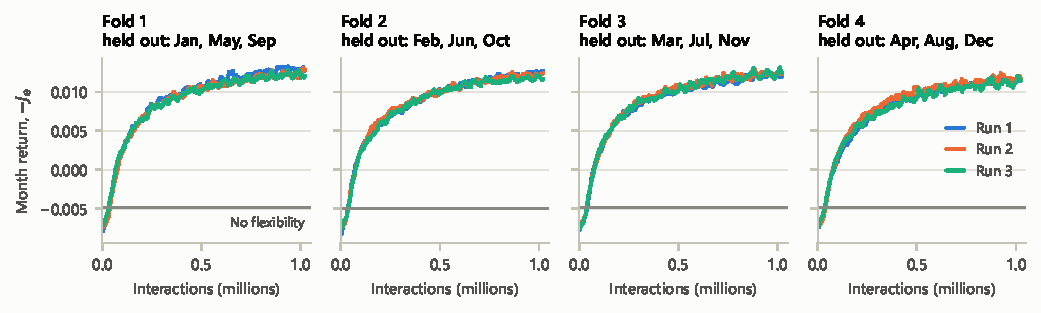
\includegraphics[width=\textwidth]{../docs/figures/ppo_cv/learning_curves.pdf}
  \caption{Return of each completed training month (\(-J_e\), higher is
  better) for each fold, averaged over the last 10 training cycles. The gray line is the
  no-flexibility baseline's return averaged over the fold's nine training
  months, \(-0.00495\) to \(-0.00486\).}
  \label{fig:learning}
\end{figure}

\section{Improvement over the Baseline}
\label{sec:results-may}

Every policy improves on the no-flexibility baseline in every held-out month
(Figure~\ref{fig:months} and Table~\ref{tab:months}). The cross-validation
estimate, the mean over the twelve months, is 0.0161 (0.0158 to 0.0165
across runs).
% [review 2026-10-21] cut three sentences read off Table 6.1: baseline J_e
% 0.0047-0.0053 and policies -0.0163 to -0.0075; largest in March and October
% (about 0.020), smallest in December (0.0133); seeds within 0.0020.

\begin{figure}[!t]
  \centering
  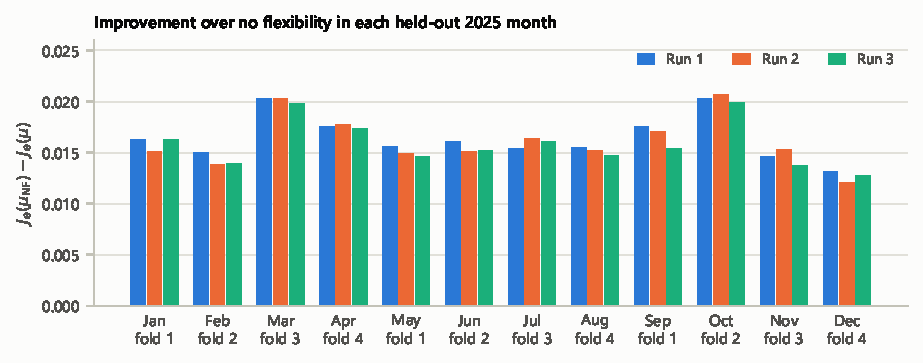
\includegraphics[width=\textwidth]{../docs/figures/ppo_cv/cv_months.pdf}
  \caption{Improvement \(J_e(\mu_{\mathrm{NF}})-J_e(\mu)\) in each 2025 month,
  scored by the final policies of the fold that held it out.}
  \label{fig:months}
\end{figure}

\begin{table}[htbp]
  \centering
  \footnotesize
  \caption{Baseline score and improvement in each held-out month, for the
  final policies of the fold that held it out. The range spans the three
  runs.}
  \label{tab:months}
  \begin{tabular}{@{}lcrrr@{}}
    \toprule
    Month (2025) & Fold & \(J_e(\mu_{\mathrm{NF}})\) & Mean improvement & Range over runs \\
    \midrule
    January   & 1 & 0.00475 & 0.0159 & 0.0151--0.0163 \\
    February  & 2 & 0.00499 & 0.0143 & 0.0138--0.0150 \\
    March     & 3 & 0.00468 & 0.0201 & 0.0198--0.0203 \\
    April     & 4 & 0.00476 & 0.0176 & 0.0174--0.0178 \\
    May       & 1 & 0.00495 & 0.0150 & 0.0147--0.0156 \\
    June      & 2 & 0.00527 & 0.0155 & 0.0151--0.0160 \\
    July      & 3 & 0.00507 & 0.0160 & 0.0154--0.0164 \\
    August    & 4 & 0.00487 & 0.0151 & 0.0147--0.0155 \\
    September & 1 & 0.00479 & 0.0167 & 0.0154--0.0175 \\
    October   & 2 & 0.00470 & 0.0203 & 0.0199--0.0207 \\
    November  & 3 & 0.00493 & 0.0146 & 0.0138--0.0153 \\
    December  & 4 & 0.00501 & 0.0127 & 0.0120--0.0132 \\
    \midrule
    All twelve &   &         & 0.0161 & 0.0158--0.0165 \\
    \bottomrule
  \end{tabular}
\end{table}

The ramp part supplies 92\% of the improvement. The peak part is positive in
34 of the 36 month--run pairs; the two exceptions, February under runs 2 and
3, are slightly negative. Table~\ref{tab:checkpoints} shows that about three quarters of both parts are
already in place at the first checkpoint, 153,600 interactions.

\begin{table}[htbp]
  \centering
  \footnotesize
  \caption{Mean improvement over the twelve held-out months by checkpoint,
  and the split of the final improvement into its weighted ramp and peak
  parts.}
  \label{tab:checkpoints}
  \begin{tabular}{@{}lrrr@{}}
    \toprule
    & Run 1 & Run 2 & Run 3 \\
    \midrule
    153,600 interactions   & 0.0123 & 0.0128 & 0.0122 \\
    512,000 interactions   & 0.0153 & 0.0154 & 0.0150 \\
    1,024,000 interactions & 0.0165 & 0.0161 & 0.0158 \\
    \midrule
    Ramp part              & 0.0152 & 0.0149 & 0.0146 \\
    Peak part              & 0.0013 & 0.0012 & 0.0012 \\
    \bottomrule
  \end{tabular}
\end{table}

% [review 2026-10-21] dropped the checkpoint figure
% (docs/figures/ppo_cv/checkpoint_improvement.pdf), which plots the first
% three rows of Table 6.2.

Relative to no flexibility, the policies cut total squared normalized ramps
by 3.1\% on average (2.1\% to 4.0\% across months) and the sum of the
markets' normalized peaks by 0.25\% (Table~\ref{tab:nf-percentages}). The peak cut
removes about a quarter of the fleet's added peak impact,
\(\sum_m\Phi_{m,e}\).

\begin{table}[htbp]
  \centering
  \footnotesize
  \caption{Mean reductions from no flexibility over the twelve held-out
  months (\%), for the final policies. Each peak is normalized by its
  market's scale before summing.}
  \label{tab:nf-percentages}
  \begin{tabular}{@{}lrrr@{}}
    \toprule
    Quantity & Run 1 & Run 2 & Run 3 \\
    \midrule
    Total squared ramps & 3.12 & 3.06 & 3.00 \\
    Total market peaks & 0.27 & 0.25 & 0.25 \\
    Fleet-added peak impact & 25.7 & 23.6 & 24.0 \\
    \bottomrule
  \end{tabular}
\end{table}

\section{Results by Market}
\label{sec:results-regions}

Table~\ref{tab:regions} gives each market's mean over the twelve months.
ISO-NE, where the site's power swing is largest relative to typical hourly
changes in net load (Table~\ref{tab:native-ramp-scale}), gains most: its squared-ramp total falls 7\% to
12\% below the original grid's, and its monthly peak falls about 100 MW below
the baseline on average. CAISO cuts its ramps by 1.4\% to 2.9\% and lowers
its peak in every month. SPP gains less on ramps but lowers its peak by about
70 MW on average. MISO, where the site's swing is smallest relative to those
changes, barely changes: its squared ramps move by less than 0.7\%, and its peak rises in 21
of the 36 month--run pairs.

% [review 2026-10-21] dropped the results-by-market figure
% (docs/figures/ppo_cv/regional_results.pdf), which shows the numbers of the
% table below.
\begin{table}[htbp]
  \centering
  \footnotesize
  \caption{Results by market for the final policies, averaged over the twelve
  held-out months: the cut in the squared one-hour ramp relative to the
  original grid, and the change in the monthly peak relative to the
  no-flexibility baseline; negative is a reduction.}
  \label{tab:regions}
  \begin{tabular}{@{}lrrrrrr@{}}
    \toprule
    & \multicolumn{3}{c}{Ramp cut (\%)}
    & \multicolumn{3}{c}{Peak change (MW)} \\
    \cmidrule(lr){2-4}\cmidrule(l){5-7}
    Market & Run 1 & Run 2 & Run 3 & Run 1 & Run 2 & Run 3 \\
    \midrule
    CAISO          & 2.0 & 2.0 & 2.0 & \(-67\) & \(-61\) & \(-66\) \\
    MISO           & \(-0.3\) & \(-0.2\) & 0.0 & \(+15\) & \(+6\) & \(+10\) \\
    SPP            & 1.3 & 1.3 & 0.8 & \(-68\) & \(-67\) & \(-68\) \\
    ISO-NE         & 10.3 & 10.3 & 9.8 & \(-112\) & \(-100\) & \(-100\) \\
    \bottomrule
  \end{tabular}
\end{table}

\section{How the Policy Achieves the Improvement}
\label{sec:results-behavior}

The policies mainly move service between sites: 29\% to 34\% of each month's
service work changes sites. Batch work waits 0.8 to 1.3 hours on average
within its 24-hour window, and the decoder adjusts the requested schedule in
64\% to 85\% of hours to meet capacity and deadline requirements.

Figure~\ref{fig:isone} shows ISO-NE over three days around its May peak hour,
under the fold-1 policy of run 2. Under the baseline, site power stays
between 272 and 305 MW. The policy runs the site near full power, about
400 MW, while net load is low and cuts it to about 164 MW as net load climbs
to its evening peak. At the peak hour it draws 165 MW, 131 MW less than the
baseline.

\begin{figure}[!t]
  \centering
  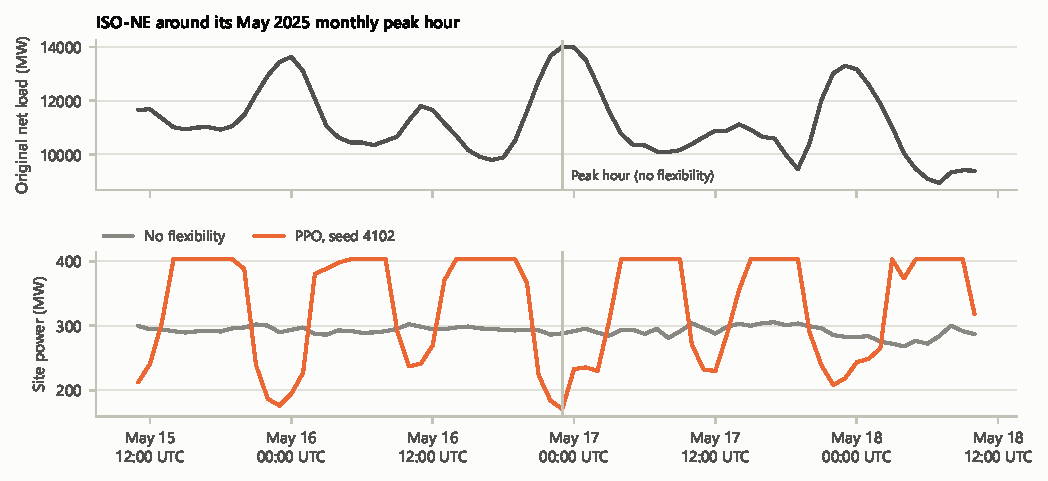
\includegraphics[width=\textwidth]{../docs/figures/ppo_cv/isone_peak_window.pdf}
  \caption{ISO-NE from 15 to 18 May 2025. Top: original net load. Bottom:
  site power under the no-flexibility baseline and the fold-1 policy of run
  2. The vertical line marks the baseline's monthly peak hour, 16 May
  23:00 UTC.}
  \label{fig:isone}
\end{figure}

\section{Test Month}
\label{sec:results-test}

% [test 2026-10-21] new section: the ten-seed final campaign on May 2026,
% numbers from docs/figures/ppo_test/test_month.json.
The ten final policies, trained on all twelve months of 2025, were scored
on May 2026, the test month, served by the test fleet of cells
\(e\)--\(h\). Every policy improves on the no-flexibility baseline
(Table~\ref{tab:test-seeds}). The mean improvement is 0.0147, from 0.0125 to
0.0171 across policies, where the baseline scores \(J_e=0.0054\). The
cross-validation estimate was 0.0161 and May 2025 scored 0.0150. The test
month has different grid data, different workload, and a larger fleet, and
the last of these puts the policies' site inputs outside their training
range, as shown below.

As in cross-validation, the ramp part supplies 92\% of the improvement, and
the peak part is positive for every policy. Relative to no flexibility, the
policies cut total squared normalized ramps by 2.9\% and the sum of the
markets' normalized peaks by 0.25\%, which removes about a fifth of the
fleet's added peak impact. \(J_e\) recomputed from the raw grid panel and
site-power trajectory differs from the reported score by at most
\(4\times10^{-17}\), and no policy left service unserved, missed a deadline,
or exceeded a site's capacity.

\begin{table}[htbp]
  \centering
  \footnotesize
  \caption{Test-month improvement of each final policy over no flexibility,
  with its weighted ramp and peak parts. The baseline scores
  \(J_e=0.00539\).}
  \label{tab:test-seeds}
  \begin{tabular}{@{}lrrr@{}}
    \toprule
    Policy & Improvement & Ramp part & Peak part \\
    \midrule
    1 & 0.0132 & 0.0120 & 0.0011 \\
    2 & 0.0125 & 0.0113 & 0.0012 \\
    3 & 0.0166 & 0.0154 & 0.0011 \\
    4 & 0.0146 & 0.0132 & 0.0014 \\
    5 & 0.0147 & 0.0135 & 0.0012 \\
    6 & 0.0139 & 0.0128 & 0.0011 \\
    7 & 0.0152 & 0.0139 & 0.0013 \\
    8 & 0.0153 & 0.0142 & 0.0011 \\
    9 & 0.0171 & 0.0158 & 0.0013 \\
    10 & 0.0135 & 0.0122 & 0.0013 \\
    \midrule
    Mean & 0.0147 & 0.0134 & 0.0012 \\
    \bottomrule
  \end{tabular}
\end{table}

Table~\ref{tab:test-markets} gives each market's results. ISO-NE again gains
most: its squared-ramp total falls 8.1\% below the original grid's on
average, and its monthly peak falls 117 MW below the baseline. CAISO's test
site, built from cell \(e\), has nearly twice the power swing of its training
site (Table~\ref{tab:native-ramp-scale}); it cuts CAISO's squared ramps by
2.7\% and its peak by 95 MW. SPP gains little: its ramps fall by 0.7\%, and its
peak rises by 15 MW on average, for six of the ten policies. MISO again barely
changes: its squared ramps move by less than 0.7\%, and its peak rises for
five of the ten policies.

\begin{table}[htbp]
  \centering
  \footnotesize
  \caption{Test-month results by market, averaged over the ten final
  policies, with the range across policies: the cut in the squared one-hour ramp
  relative to the original grid, and the change in the monthly peak relative
  to the no-flexibility baseline; negative is a reduction.}
  \label{tab:test-markets}
  \begin{tabular}{@{}lrrrr@{}}
    \toprule
    & \multicolumn{2}{c}{Ramp cut (\%)} & \multicolumn{2}{c}{Peak change (MW)} \\
    \cmidrule(lr){2-3}\cmidrule(l){4-5}
    Market & Mean & Range & Mean & Range \\
    \midrule
    CAISO          & 2.7 & 2.4 to 3.3 & \(-95\) & \(-110\) to \(-76\) \\
    MISO           & \(-0.3\) & \(-0.6\) to 0.2 & \(+8\) & \(-81\) to \(+134\) \\
    SPP            & 0.7 & 0.0 to 1.4 & \(+15\) & \(-30\) to \(+61\) \\
    ISO-NE         & 8.1 & 5.0 to 9.2 & \(-117\) & \(-133\) to \(-97\) \\
    \bottomrule
  \end{tabular}
\end{table}

% [raw-obs 2026-10-27] added: the test fleet's site inputs fall outside the
% training range; numbers from site_arrival_range in test_month.json.
One difference between the test month and cross-validation shows in the site
inputs. The test fleet's sites are larger than the training fleet's
(Table~\ref{tab:active-market-map}), and the observation gives each site's
arrivals, queued work, and power in their own units
(Section~\ref{sec:method-observation}), so in the test month these entries
are larger than any the policies saw in training. After the library's
rescaling, the test sites' service and batch arrivals lie on average 2.9
standard deviations from their training averages, against 0.8 in a training
month, and 40\% of them lie more than 3 standard deviations away, against
almost none in training. The grid entries stay in their usual range. The
policies are therefore acting on site inputs outside the range they learned
from. Cross-validation cannot show this, because every 2025 month is served by
the same fleet.

The policies act much as in cross-validation, though with a wider spread:
25\% to 34\% of the month's service work changes sites, batch work waits 0.5
to 1.4 hours on average, and the decoder adjusts the requested schedule in
44\% to 87\% of hours. Each final policy trained for 1,024,000 interactions in
54 to 116 minutes, and its training return, averaged over its last 10
training cycles, ends between 0.0107 and 0.0126, close to the cross-validation
runs' 0.0115 to 0.0129.

\section{Ablations and Comparisons}
\label{sec:results-comparisons}

\planned{comparison runs from sec.~\ref{sec:method-comparisons}}

\chapter{DISCUSSION AND CONCLUSIONS}
\label{chap:discussion}

\section{Summary of Findings}
\label{sec:discussion-findings}

% [ch7 2026-10-21] wrote 7.1, 7.2, 7.4, and 7.5 from the cross-validation and
% test-month results, and added the last two limitations in 7.3.
The question in Section~\ref{sec:intro-questions} asked how much a causal
scheduler can smooth each market's one-hour net-load ramps and reduce its
monthly peak by deferring and routing work within the service, deadline, and
capacity limits. For the fleet modeled here, the answer is an improvement
that appears in every month scored but is modest in size:
\begin{itemize}
  \item The trained policies improve on no flexibility in every month. The
        cross-validation estimate over the twelve months of 2025 is 0.0161,
        and the ten final policies score 0.0147 on the May 2026 test month,
        every policy between 0.0125 and 0.0171.
  \item About 92\% of the improvement comes from ramps. Total squared
        normalized ramps fall by 3.1\% in cross-validation and 2.9\% in the
        test month. The markets' summed peaks fall by less than 0.3\%, which
        removes about a quarter of the fleet's added peak impact in
        cross-validation and about a fifth in the test month.
  \item The policies act mainly by routing service: 25\% to 34\% of each
        month's service work changes sites, while batch work waits only 0.5 to
        1.4 hours on average within its 24-hour window. No run separates the
        two levers, so this describes what the policies do, not which lever
        produces the improvement.
  \item The largest and smallest gains match the fleet's size relative to
        each market's hourly changes in net load
        (Table~\ref{tab:native-ramp-scale}). ISO-NE, where a site's swing is
        about half of a typical hourly change, gains most: its squared ramps
        fall by 8\% to 10\%, and its peak ends 100 to 120 MW below the
        baseline. MISO, where a site's swing is a tenth to a fifth of a typical
        change, barely changes, and its peak rises about as often as it falls.
        CAISO and SPP lie between. CAISO's test site has about twice the swing
        of its training site, and CAISO's gains are larger in the test month:
        a 2.7\% ramp cut against 2.0\%, and 95 MW off the peak against 65 MW.
  \item The test month scores below the cross-validation estimate. Its sites
        are larger than the training sites, and because the observation gives
        site quantities in their own units, the policies see site inputs
        outside the range they trained on (Section~\ref{sec:results-test}).
\end{itemize}

\section{Interpretation for Fleet and Grid Operators}
\label{sec:discussion-interpretation}

The peak results are easiest to read in MW. In the test month, the fleet
without flexibility raises ISO-NE's monthly net-load peak by 425 MW, from
17,506 to 17,931 MW, and CAISO's by 299 MW. The policies remove 117 MW of the
ISO-NE increase and 95 MW of the CAISO increase, about 30\% of what the fleet
adds in each. In SPP and MISO they do not reduce the peak, which ends slightly
higher than without flexibility. The fleet still raises every market's peak above that of the grid
alone: flexibility shrinks the data centers' contribution to the peak rather
than lowering the peak below what the grid would see without them.

The ramp results depend on where the fleet is large relative to the grid. In
ISO-NE, the total squared one-hour ramp ends 8\% to 10\% below that of the
grid without the fleet. In MISO, whose typical hourly change is several times
a site's swing, the fleet has almost no effect. For a fleet operator, the
results show in which markets a fleet of this size can change the shape of
net load, and by how much.

The gains are reported as changes in the modeled score and in MW, not as
cost or reliability savings. Electricity prices, capacity charges, ramping
products, and reserve requirements are not modeled
(Section~\ref{sec:intro-scope}), and the value of a lower peak or a smoother
ramp depends on each market's rules. Turning these changes into savings would
require those rules.

\section{Limitations}
\label{sec:limitations}

The study has the following limitations:
\begin{itemize}
  \item The trace is replayed from its first day in every month, so its
        weekdays do not match the month's: 1 May 2019 was a Wednesday, while
        February 2025, for example, starts on a Saturday.
  \item The workload comes from one company and one month in 2019, and
        measured execution is reused as synthetic arrival demand. Every 2025
        month replays the same workload of cells \(a\)--\(d\), so
        cross-validation tests new grid months but not new workload; only the
        test month, with cells \(e\)--\(h\), tests unseen workload.
  \item The service/batch split, completion windows, the 500 MW scale of the
        site built from cell \(c\), the assumption that power capacity scales
        with CPU capacity, and the cell-to-market mapping all include
        modeling assumptions.
  \item The forecasts are simple least-squares regressions fitted here on
        public EIA data.
        An operator would hold system-operator or commercial forecasts of
        different accuracy, and the scheduler's benefit may depend on that
        accuracy.
  \item Routing remains free and instantaneous, making the available
        geographic flexibility optimistic.
  \item The test is one month. In 2025, the improvement in a single month
        ranged from 0.0127 to 0.0203 (Table~\ref{tab:months}), so the test
        month's 0.0147 carries month-to-month variation of about that size.
  \item The observation gives each site's arrivals, queued work, and power in
        their own units, so a policy trained on one fleet sees inputs outside
        its training range when the sites are larger, as the test fleet's are
        (Section~\ref{sec:results-test}).
  \item The PPO settings are the library's defaults and were not tuned for
        this problem (Section~\ref{sec:method-training}), so better settings
        may exist.
\end{itemize}

\section{Future Work}
\label{sec:discussion-future}

Several extensions follow from these results:
\begin{itemize}
  \item Ramp-only and peak-only policies (Section~\ref{sec:method-comparisons})
        would show how much each part of the objective drives the other's
        gains, and a variant in which service stays at its own site and only
        batch work moves would show what deferral alone achieves.
  \item A simple forecast-aware rule, using the same observations, workload
        constraints, and feasibility decoder, would show what learning adds
        beyond flexible scheduling.
  \item Routing costs, latency, and limits on how much work can move would
        make the geographic flexibility less optimistic.
  \item More test months, other years, and workload from other cells or
        operators would test whether the gains hold beyond one month of one
        company's workload.
  \item Electricity prices or carbon signals could be added to the objective
        alongside ramps and peaks, and cooling control or on-site generation
        would give the scheduler more levers.
  \item Giving each site's arrivals, queued work, and power as shares of its
        capacity would make the observation the same for sites of any size,
        so that policies trained on one fleet could carry over to another.
  \item Tuned PPO settings, the action range of \([-1,1]\) that the library's
        guide recommends, or other learning algorithms may improve on the
        untuned policies.
\end{itemize}

\section{Conclusions}
\label{sec:discussion-conclusions}

A four-site data-center fleet built from public Google and EIA data was used
to test whether a learned scheduler can smooth grid ramps and lower monthly
net-load peaks while running all work within its service, deadline, and
capacity limits. A PPO policy that routes service and defers batch work
improved the joint ramp-and-peak score over running all work where and when
it arrives in every month tested: by 0.0161 on average over the
cross-validation months of 2025, and by 0.0147 in the held-out test month,
whose larger sites put the policies' site inputs outside their training
range.
Most of the gain is in ramps, and it is largest where the fleet is large
relative to the grid, as in ISO-NE. The fleet still adds to every market's
peak, but flexibility removes about 30\% of that addition in the markets
where it matters most. Because routing is free and the workload comes from
one month of one company, these results show what such flexibility can do in
an optimistic setting, not what a real fleet would save.

% References and appendices use the front-matter heading format (1-inch top
% margin), as in the template's example thesis.
\fbmatterchapterformat

\begin{thebibliography}{99}

% \bibitem{iea2026energyai}
% International Energy Agency, ``Key Questions on Energy and AI,'' World Energy
% Outlook Special Report, IEA, Paris, France, 2026. [Online]. Available:
% \url{https://www.iea.org/reports/key-questions-on-energy-and-ai}.
% Accessed: Jun. 11, 2026.

% \bibitem{vasques2019review}
% T. L. Vasques, P. Moura, and A. de Almeida, ``A review on energy efficiency
% and demand response with focus on small and medium data centers,''
% \emph{Energy Efficiency}, vol. 12, no. 5, pp. 1399--1428, 2019,
% doi: 10.1007/s12053-018-9753-2.

% \bibitem{sakalkar2020oversubscription}
% V. Sakalkar, V. Kontorinis, D. Landhuis, S. Li, D. De Ronde, T. Blooming,
% A. Ramesh, J. Kennedy, C. Malone, J. Clidaras, and P. Ranganathan, ``Data
% center power oversubscription with a medium voltage power plane and
% priority-aware capping,'' in \emph{Proc. 25th Int. Conf. Architectural
% Support for Programming Languages and Operating Systems (ASPLOS)}, 2020,
% pp. 497--511, doi: 10.1145/3373376.3378533.

% \bibitem{qureshi2009cutting}
% A. Qureshi, R. Weber, H. Balakrishnan, J. Guttag, and B. Maggs, ``Cutting the
% electric bill for internet-scale systems,'' in \emph{Proc. ACM SIGCOMM},
% 2009, pp. 123--134, doi: 10.1145/1592568.1592584.

% \bibitem{rao2010minimizing}
% L. Rao, X. Liu, L. Xie, and W. Liu, ``Minimizing electricity cost:
% Optimization of distributed internet data centers in a
% multi-electricity-market environment,'' in \emph{Proc. IEEE INFOCOM}, 2010,
% pp. 1145--1153.

% \bibitem{liu2011glb}
% Z. Liu, M. Lin, A. Wierman, S. H. Low, and L. L. H. Andrew, ``Geographical
% load balancing with renewables,'' \emph{ACM SIGMETRICS Perform. Eval. Rev.},
% vol. 39, no. 3, pp. 62--66, 2011, doi: 10.1145/2160803.2160862.

% \bibitem{zhao2025cfws}
% D. Zhao, J.-T. Zhou, and K. Li, ``CFWS: DRL-based framework for energy cost
% and carbon footprint optimization in cloud data centers,'' \emph{IEEE Trans.
% Sustain. Comput.}, vol. 10, no. 1, pp. 95--107, 2025,
% doi: 10.1109/TSUSC.2024.3391791.

% \bibitem{liu2012renewable}
% Z. Liu, Y. Chen, C. Bash, A. Wierman, D. Gmach, Z. Wang, M. Marwah, and
% C. Hyser, ``Renewable and cooling aware workload management for sustainable
% data centers,'' in \emph{Proc. 12th ACM SIGMETRICS/PERFORMANCE Joint Int.
% Conf. Measurement and Modeling of Computer Systems}, 2012, pp. 175--186,
% doi: 10.1145/2254756.2254779.

% \bibitem{grange2018green}
% L. Grange, G. Da Costa, and P. Stolf, ``Green IT scheduling for data center
% powered with renewable energy,'' \emph{Future Gener. Comput. Syst.}, vol. 86,
% pp. 99--120, 2018, doi: 10.1016/j.future.2018.03.049.

% \bibitem{xu2021selfadaptive}
% M. Xu, A. N. Toosi, and R. Buyya, ``A self-adaptive approach for managing
% applications and harnessing renewable energy for sustainable cloud
% computing,'' \emph{IEEE Trans. Sustain. Comput.}, vol. 6, no. 4,
% pp. 544--558, 2021, doi: 10.1109/TSUSC.2020.3014943.

\bibitem{haghshenas2022infrastructure}
K. Haghshenas, S. Taheri, M. Goudarzi, and S. Mohammadi, ``Infrastructure
aware heterogeneous-workloads scheduling for data center energy cost
minimization,'' \emph{IEEE Trans. Cloud Comput.}, vol. 10, no. 2,
pp. 972--983, 2022, doi: 10.1109/TCC.2020.2977040.

\bibitem{radovanovic2021carbonaware}
A. Radovanovi\'{c} \emph{et al.}, ``Carbon-Aware Computing for Datacenters,''
arXiv:2106.11750v1, 2021. [Online]. Available:
\url{https://arxiv.org/abs/2106.11750v1}.

% \bibitem{kahil2025rl}
% H. Kahil, S. Sharma, P. V\"{a}lisuo, and M. Elmusrati, ``Reinforcement
% learning for data center energy efficiency optimization: A systematic
% literature review and research roadmap,'' \emph{Appl. Energy}, vol. 389,
% Art. no. 125734, 2025, doi: 10.1016/j.apenergy.2025.125734.

% \bibitem{vazquezcanteli2019demand}
% J. R. V\'{a}zquez-Canteli and Z. Nagy, ``Reinforcement learning for demand
% response: A review of algorithms and modeling techniques,'' \emph{Appl.
% Energy}, vol. 235, pp. 1072--1089, 2019, doi: 10.1016/j.apenergy.2018.11.002.

% \bibitem{ran2019deepee}
% Y. Ran, H. Hu, X. Zhou, and Y. Wen, ``DeepEE: Joint optimization of job
% scheduling and cooling control for data center energy efficiency using deep
% reinforcement learning,'' in \emph{Proc. IEEE Int. Conf. Distributed
% Computing Systems (ICDCS)}, 2019, pp. 645--655,
% doi: 10.1109/ICDCS.2019.00070.

% \bibitem{naug2024sustaindc}
% A. Naug \emph{et al.}, ``SustainDC: Benchmarking for sustainable data center
% control,'' in \emph{Advances in Neural Information Processing Systems},
% vol. 37, Datasets and Benchmarks Track, 2024,
% doi: 10.52202/079017-3192.

% \bibitem{zhang2018practical}
% Z. Zhang and K. P. Lam, ``Practical implementation and evaluation of deep
% reinforcement learning control for a radiant heating system,'' in
% \emph{Proc. 5th ACM Int. Conf. Systems for Built Environments (BuildSys)},
% 2018, pp. 148--157, doi: 10.1145/3276774.3276775.

\bibitem{wilkes2020clusterdata2019}
J. Wilkes, ``Google cluster-usage traces v3,'' 2020. [Online]. Available:
\url{https://github.com/google/cluster-data/blob/master/ClusterData2019.md}.
Accessed: Aug. 28, 2026.

\bibitem{tirmazi2020borg}
M. Tirmazi, A. Barker, N. Deng, M. E. Haque, Z. G. Qin, S. Hand,
M. Harchol-Balter, and J. Wilkes, ``Borg: The next generation,'' in
\emph{Proc. 15th Eur. Conf. Comput. Syst. (EuroSys)}, 2020, pp. 1--14,
doi: 10.1145/3342195.3387517.

% \bibitem{dacosta2016modeling}
% G. Da Costa, L. Grange, and I. De Courchelle, ``Modeling and generating
% large-scale Google-like workload,'' in \emph{Proc. 7th Int. Green and
% Sustainable Computing Conf. (IGSC)}, 2016, pp. 1--7,
% doi: 10.1109/IGCC.2016.7892623.

% \bibitem{lin2024systematic}
% W. Lin, J. Lin, Z. Peng, H. Huang, W. Lin, and K. Li, ``A systematic review
% of green-aware management techniques for sustainable data center,''
% \emph{Sustain. Comput.: Informat. Syst.}, vol. 42, Art. no. 100989, 2024,
% doi: 10.1016/j.suscom.2024.100989.

% \bibitem{dayarathna2016survey}
% M. Dayarathna, Y. Wen, and R. Fan, ``Data center energy consumption modeling:
% A survey,'' \emph{IEEE Commun. Surveys Tuts.}, vol. 18, no. 1, pp. 732--794,
% 2016, doi: 10.1109/COMST.2015.2481183.

% \bibitem{zhang2021cooling}
% Q. Zhang, Z. Meng, X. Hong, Y. Zhan, J. Liu, J. Dong, T. Bai, J. Niu, and
% M. J. Deen, ``A survey on data center cooling systems: Technology, power
% consumption modeling and control strategy optimization,'' \emph{J. Syst.
% Archit.}, vol. 119, Art. no. 102253, 2021,
% doi: 10.1016/j.sysarc.2021.102253.

% \bibitem{zhang2016joint}
% W. Zhang, Y. Wen, Y. W. Wong, K. C. Toh, and C.-H. Chen, ``Towards joint
% optimization over ICT and cooling systems in data centre: A survey,''
% \emph{IEEE Commun. Surveys Tuts.}, vol. 18, no. 3, pp. 1596--1616, 2016,
% doi: 10.1109/COMST.2016.2545109.

% \bibitem{katal2023energy}
% A. Katal, S. Dahiya, and T. Choudhury, ``Energy efficiency in cloud computing
% data centers: A survey on software technologies,'' \emph{Cluster Comput.},
% vol. 26, pp. 1845--1875, 2023, doi: 10.1007/s10586-022-03713-0.

% \bibitem{panwar2022systematic}
% S. S. Panwar, M. M. S. Rauthan, and V. Barthwal, ``A systematic review on
% effective energy utilization management strategies in cloud data centers,''
% \emph{J. Cloud Comput.}, vol. 11, Art. no. 95, 2022,
% doi: 10.1186/s13677-022-00368-5.

\bibitem{googlePowerData2019}
Google, ``PowerData2019: power measurements for ClusterData2019,'' 2020.
[Online]. Available:
\url{https://github.com/google/cluster-data/blob/master/PowerData2019.md}.
Accessed: Sep. 7, 2026.

\bibitem{googleTraceFormatV3}
Google, ``ClusterData trace format v3,'' protocol-buffer schema, 2019.
[Online]. Available:
\url{https://github.com/google/cluster-data/blob/master/clusterdata_trace_format_v3.proto}.
Accessed: Aug. 28, 2026.

\bibitem{googleClusterAnalysisColab}
Google, ``Google trace analysis Colab,'' 2020. [Online]. Available:
\url{https://github.com/google/cluster-data/blob/master/clusterdata_analysis_colab.ipynb}.
Accessed: Aug. 28, 2026.

\bibitem{googlePowerTraceDocumentation}
J. Prakash and V. Kontorinis, ``Google Data Center Power Trace,''
Feb. 15, 2024, p.~2. [Online]. Available:
\url{https://raw.githubusercontent.com/google/cluster-data/master/power_trace_documentation.pdf}.
Accessed: Sep. 15, 2026.

\bibitem{eiaGridMonitor}
U.S. Energy Information Administration, ``Hourly Electric Grid Monitor.''
[Online]. Available: \url{https://www.eia.gov/electricity/gridmonitor/}.
Accessed: Aug. 28, 2026.

% \bibitem{hastie2009elements}
% T. Hastie, R. Tibshirani, and J. Friedman, \emph{The Elements of Statistical
% Learning: Data Mining, Inference, and Prediction}, 2nd ed. New York, NY, USA:
% Springer, 2009, Sec.~7.10.

% \bibitem{bergmeir2012crossvalidation}
% C. Bergmeir and J. M. Ben\'{\i}tez, ``On the use of cross-validation for time
% series predictor evaluation,'' \emph{Inf. Sci.}, vol. 191, pp. 192--213, 2012.

\bibitem{sutton2018reinforcement}
R. S. Sutton and A. G. Barto, \emph{Reinforcement Learning: An Introduction},
2nd ed. Cambridge, MA, USA: MIT Press, 2018.

% \bibitem{markgraf2026projection}
% H. Markgraf, S. Sawant, H. Krasowski, L. Sch\"{a}fer, S. Gros, and M. Althoff,
% ``Safe reinforcement learning using action projection: Safeguard the policy or
% the environment?,'' \emph{Trans. Mach. Learn. Res.}, 2026. [Online].
% Available: \url{https://arxiv.org/abs/2509.12833}.

\bibitem{schulman2017ppo}
J. Schulman, F. Wolski, P. Dhariwal, A. Radford, and O. Klimov, ``Proximal
policy optimization algorithms,'' arXiv:1707.06347, 2017.

\bibitem{schulman2016gae}
J. Schulman, P. Moritz, S. Levine, M. Jordan, and P. Abbeel,
``High-dimensional continuous control using generalized advantage
estimation,'' in \emph{Proc. Int. Conf. Learn. Represent. (ICLR)}, 2016.

\bibitem{raffin2021sb3}
A. Raffin, A. Hill, A. Gleave, A. Kanervisto, M. Ernestus, and N. Dormann,
``Stable-Baselines3: Reliable reinforcement learning implementations,''
\emph{J. Mach. Learn. Res.}, vol. 22, no. 268, pp. 1--8, 2021.

\bibitem{sb3ppodocs}
Stable-Baselines3 contributors, ``PPO,'' Stable-Baselines3 documentation,
version 2.9.0. [Online]. Available:
\url{https://stable-baselines3.readthedocs.io/en/master/modules/ppo.html}.
Accessed: Oct. 19, 2026.

\bibitem{sb3tips}
Stable-Baselines3 contributors, ``Reinforcement learning tips and tricks,''
Stable-Baselines3 documentation, version 2.9.0. [Online]. Available:
\url{https://stable-baselines3.readthedocs.io/en/master/guide/rl_tips.html}.
Accessed: Oct. 19, 2026.

\end{thebibliography}

% Appendix headings read "APPENDIX A: TITLE"; sections inside the appendices
% are left out of the table of contents.
\clearpage
\uncctocformat{chapter}{0pt}{350pt}{\appendixname~\thecontentslabel:~}
\renewcommand{\chaptertitlename}{APPENDIX}
\addtocontents{toc}{\protect\setcounter{tocdepth}{0}}
\appendix

\chapter{DATA SCHEMAS}
\label{app:data-schemas}

The tables below document the stored workload curves and hourly grid panels.

\section{Five-Minute Workload Curves}
Each stored curve contains 8,929 rows. The final row is dropped because it
cannot form a complete group of twelve, leaving 744 whole hours.

\begingroup
\small
\singlespacing
\begin{longtable}{@{}L{0.22\textwidth}L{0.39\textwidth}rrr@{}}
\caption{Stored workload columns for cell \(a\), with examples at minimum,
  median, and maximum CPU utilization. The example rows are not consecutive.}
  \label{tab:clusterdata-tier-columns}\\
    \toprule
     & & \multicolumn{3}{c}{Cell \(a\)} \\
    \cmidrule(l){3-5}
    Column & Meaning & Quiet & Median & Busy \\
    \midrule
  \endfirsthead
    \toprule
     & & \multicolumn{3}{c}{Cell \(a\)} \\
    \cmidrule(l){3-5}
    Column & Meaning & Quiet & Median & Busy \\
    \midrule
  \endhead
    \codepath{timestep}
      & Five-minute index in the stored curve.
      & 255 & 5257 & 2681 \\
    \addlinespace
    \codepath{cpu_demand_norm}
      & All retained CPU use divided by the cell's reference capacity,
        \(u_{\mathrm{cell},k}\).
      & 0.3320 & 0.5652 & 0.6931 \\
    \addlinespace
    \codepath{service_demand_norm}
      & CPU use not classified as batch, including work with no recorded
        priority, \(u^{\mathrm{svc}}_{\mathrm{cell},k}\).
      & 0.2432 & 0.4416 & 0.6341 \\
    \addlinespace
    \codepath{batch_demand_norm}
      & CPU use by jobs with priority 115 or below,
        \(u^{\mathrm{bat}}_{\mathrm{cell},k}\).
      & 0.0888 & 0.1236 & 0.0590 \\
    \bottomrule
\end{longtable}
\endgroup


\section{Hourly Grid Panels}
For each month, which runs from 07:00 UTC on its first day
(Section~\ref{subsec:transform-pairing}), the simulation uses the month's grid
rows and the immediately preceding hour. Workload arrivals are attached separately as
described in Section~\ref{subsec:transform-pairing}. The committed 2025
panels hold the final scales and forecasts, fitted on all of 2025; each
cross-validation fold writes its own copies with its own scales and
forecasts, and the May 2026 test panel has the same columns.

\begingroup
\small
\singlespacing
\begin{longtable}{@{}L{0.23\textwidth}L{0.36\textwidth}r@{}}
\caption{Example hourly grid record for CAISO, 2025-07-19 16:00 UTC.}
  \label{tab:panel-columns}\\
    \toprule
    Column & Meaning & Value \\
    \midrule
  \endfirsthead
    \toprule
    Column & Meaning & Value \\
    \midrule
  \endhead
    \codepath{timestamp_utc}
      & Beginning of the UTC hour the row describes.
      & 2025-07-19 16:00Z \\
    \codepath{market_id}
      & Market.
      & \codepath{CAISO} \\
    \addlinespace
    \codepath{gross_demand_mw}
      & Balancing-authority demand, \(D_m\) (EIA series \codepath{D}).
      & 29,214 \\
    \codepath{wind_mw}
      & Observed wind generation, \(G^{\mathrm{wnd}}_m\) (EIA series
        \codepath{NG.WND}).
      & 2,096 \\
    \codepath{solar_mw}
      & Observed solar generation, \(G^{\mathrm{sol}}_m\) (EIA series
        \codepath{NG.SUN}).
      & 15,279 \\
    \codepath{net_load_mw}
      & Net load \(N_m\) from Equation~\eqref{eq:energy-net-load}.
      & 11,839 \\
    \addlinespace
    \codepath{market_scale_mw}
      & Ramp and peak normalizer \(S_m\) from Equation~\eqref{eq:market-scale};
        constant within a market.
      & 33,781 \\
    \addlinespace
    \codepath{forecast_gross_h1/h3/h6/h12_mw}
      & Gross-demand forecast at each of the four lead times, from
        Equation~\eqref{eq:forecast-model}.
      & 30,396 / 31,019 / 29,981 / 32,612 \\
    \codepath{forecast_net_h1/h3/h6/h12_mw}
      & Net-load forecast at each of the four lead times, from
        Equation~\eqref{eq:forecast-model}.
      & 11,183 / 11,508 / 10,571 / 28,166 \\
    \codepath{forecast_issue_time_utc},
    \codepath{forecast_vintage_id},
    \codepath{quality_ok}
      & Forecast provenance and quality checks.
      & --- \\
    \bottomrule
\end{longtable}
\endgroup

\chapter{IMPLEMENTATION NOTES}
\label{app:implementation}
% Ragged right: long code names cannot be hyphenated and would otherwise run
% into the margin. \raggedright zeroes \parindent, so it is restored.
\raggedright
\setlength{\parindent}{.17in}

Paths are relative to the repository root. Several names predate the current
design: \codepath{energy_model_v3}, \codepath{env/ramp_v6},
and the \codepath{four_market_v2} prefix. The market identifiers are
\codepath{CAISO}, \codepath{MISO}, \codepath{SPP}, and \codepath{ISONE}.
\codepath{env/ramp_v6/clock.py} defines the month clock of
Section~\ref{subsec:transform-pairing}, a fixed UTC\(-7\); every script that
splits hours into months uses it. \codepath{README.md} gives the rebuild
commands. The last two sections cover the training, evaluation, and figure code of
Chapters~\ref{chap:method} and~\ref{chap:results}.

\section{Workload Extraction (Sections~\ref{sec:clusterdata2019}--\ref{subsec:clusterdata-tier-split})}
\begin{itemize}
  \item \codepath{extract_cells.ipynb} runs the BigQuery queries in
        Google Colab or a local Jupyter kernel.
  \item The trace's tables are \codepath{machine_events} (the machine list),
        \codepath{instance_usage} (the task usage measurements), and
        \codepath{collection_events} (the job records). The fields used are
        \codepath{capacity.cpus}, a machine's CPU capacity on the scale of
        Section~\ref{subsec:clusterdata-capacity};
        \codepath{average_usage.cpus}, the average CPU used during one
        measurement, \(a_r\); \codepath{start_time} and
        \codepath{end_time}, the measurement window; and
        \codepath{alloc_collection_id}, the allocation set a task runs in,
        which is empty or 0 for tasks outside any set and for the reserved
        blocks themselves.
  \item The query's \codepath{cap} step, a common-table expression (a named
        sub-query), computes
        \(C^{\mathrm{ref}}_{\mathrm{cell}}\) (Equation~\eqref{eq:reference-capacity}) by
        taking \codepath{MAX(capacity.cpus)} for each \codepath{machine_id}
        and summing over machines. The capacity cell sums the same
        per-machine maxima, counting machines that report both a CPU and a
        memory capacity, and saves the result, with each cell's machine count, to
        \codepath{data/cell_capacity.json}, which sets the site sizes in
        Table~\ref{tab:active-market-map}.
  \item The usage query assigns each row to a 300-second bucket by
        \codepath{start_time}, sums \codepath{average_usage.cpus}, divides by
        \(C^{\mathrm{ref}}_{\mathrm{cell}}\), and clips the result to \([0,1]\), a bound no
        retained bucket reaches. Its \codepath{WHERE} clause keeps rows whose
        \codepath{alloc_collection_id} is empty or 0, which drops tasks
        running inside an allocation set and keeps the blocks, and requires
        \codepath{end_time-start_time} of at least 300 seconds.
  \item The \codepath{prio} step takes, for each job
        (\codepath{collection_id}), the highest priority among its
        submission events, which have \codepath{type=0}. A left join keeps
        usage rows with no matching priority, and those count as service.
  \item \codepath{scripts/bigquery/audit_300s_filter.sql} audits the
        300-second filter with the same top-level filter and priority join.
        Its first query measures the rows and CPU work removed by cell and
        class, saved as
        \codepath{scripts/bigquery/results/query1_filter_volume.csv}; its
        second compares hourly level, one-hour ramps, and peaks with and
        without the filter, saved as
        \codepath{scripts/bigquery/results/query2_hourly_shape.csv}. Work is
        \codepath{average_usage.cpus} times window duration.
  \item The notebook writes \codepath{data/cells/cell_a_tiers.csv} through
        \codepath{data/cells/cell_h_tiers.csv}. \codepath{TRAIN_CELLS} lists
        \(a\)--\(d\) and \codepath{TEST_CELLS} lists \(e\)--\(h\); setting
        \codepath{INCLUDE_TEST_CELLS = False} extracts only the training
        cells.
\end{itemize}

\section{Power Model (Section~\ref{sec:powerdata2019})}
\begin{itemize}
  \item The power-extraction cell of
        \codepath{extract_cells.ipynb} averages
        \codepath{measured_power_util} by hour from \codepath{powerdata_2019},
        excluding rows flagged \codepath{bad_measurement_data}. It builds hourly
        CPU utilization with the filters above and fits each cell with
        \codepath{numpy.linalg.lstsq}.
  \item Coefficients are stored under \codepath{per_cell_cpu_model} in
        \codepath{data/power_model_params.json} as \codepath{idle_power}
        (\(\alpha_{\mathrm{cell}}\)), \codepath{slope} (\(\beta_{\mathrm{cell}}\)), \codepath{r_squared},
        and the number of fitted hours, \codepath{n}, for all eight cells.
  \item \codepath{_site_configs} in
        \codepath{scripts/build_four_market_v2_factory.py} copies
        \(\alpha_m,\beta_m\) into each site's \codepath{SiteConfig}, whose
        \codepath{power_mw} method in \codepath{env/ramp_v6/models.py}
        evaluates Equation~\eqref{eq:runtime-power}.
\end{itemize}

\section{Grid Data and Forecasts (Sections~\ref{sec:energy-data}--\ref{subsec:energy-forecasts})}
\begin{itemize}
  \item \codepath{scripts/fetch_eia_panels.py} downloads the series from the
        EIA API v2 with the key \codepath{EIA_API_KEY} in an untracked
        \codepath{.env} file. \codepath{MARKETS} maps each market to its EIA
        balancing-authority code, \codepath{CISO},
        \codepath{MISO}, \codepath{SWPP}, and \codepath{ISNE}, and \codepath{fetch_series} requests demand from
        \codepath{region-data} and wind and solar from
        \codepath{fuel-type-data}. \codepath{HOUR_LABEL_IS_ENDING} applies the
        one-hour shift.
  \item \codepath{build_frame} clips negative wind and solar values to
        zero and computes \codepath{net_load_mw}.
  \item \codepath{write_panels} writes
        \codepath{data/four_market_2025/months/YYYY-MM/canonical_panel.csv},
        holding the warm-up hour and the month, and
        \codepath{data/four_market_2025/calendar.json}, which lists the
        twelve 2025 months, the folds, and the test month. The same split
        appears under \codepath{data.split} in
        \codepath{env/protocols/four_market_v2.yaml}, the single protocol
        file, and a test keeps both in step with
        \codepath{energy_model_v3/splits.py}. \codepath{--test-raw} fetches
        23~April to 18:00 UTC on 1~June 2026 into
        \codepath{data/four_market_2026_test/raw_hourly.csv}.
  \item \codepath{frozen_stats} in \codepath{energy_model_v3/splits.py}
        computes \(S_m\) from a given set of training months, together with
        level means and standard deviations that only the scaled-observation
        option below uses. The final values, from all of 2025, are stored in
        \codepath{data/four_market_2025/frozen_stats.json}, with \(S_m\) as
        \codepath{gross_q95_mw}, and \(S_m\) is repeated as
        \codepath{market_scale_mw} in every panel row.
  \item \codepath{CanonicalMarketPanel} in \codepath{env/ramp_v6/panel.py}
        checks that the columns in \codepath{REQUIRED_COLUMNS} are present and
        finite, that timestamps are contiguous hourly UTC with every market in
        every hour, and that no forecast is issued after its row's hour.
  \item \codepath{scripts/build_causal_forecasts.py} implements
        Section~\ref{subsec:energy-forecasts}. \codepath{INPUT_SETS} holds
        the five candidate input sets and \codepath{INPUT_SET} the chosen
        one. \codepath{build_features} constructs a set's inputs for one
        quantity and lead, \codepath{assert_causal} stops the build if any
        input uses a later hour, \codepath{fit_rows} keeps only rows whose inputs and target
        all lie in training months, and \codepath{fit_least_squares} fits the
        weights of Equation~\eqref{eq:forecast-model} with the least-squares
        solver of the numpy library. \codepath{fit_forecasts} fits all 32
        models on any set of training months and flags any that fail to beat
        persistence on their training rows. \codepath{predict}
        applies fixed weights to any hourly series, filling rows without a
        week of history with persistence. \codepath{--select} prints the
        cross-validation comparison of the candidate input sets,
        \codepath{--report} prints the
        cross-validation and test accuracy of
        Table~\ref{tab:forecast-accuracy}, and \codepath{--write} writes the
        final forecasts into the 2025 panels and builds the test panel
        \codepath{data/four_market_2026_test/months/2026-05/canonical_panel.csv},
        recording the vintage \codepath{causal-least-squares-v4} in
        \codepath{calendar.json}.
  \item Forecast lead times are \codepath{FORECAST_HOURS} and urgency horizons
        are \codepath{deadline_bucket_hours}, both in
        \codepath{env/ramp_v6/models.py}. \codepath{EDFQueue.due_by} computes
        urgency.
  \item \codepath{scripts/build_data_figures.py} draws
        Figures~\ref{fig:workload-week} and~\ref{fig:net-load-week} from the
        tier curves and the July 2025 panel into
        \codepath{docs/figures/data/}.
\end{itemize}

\section{Cross-Validation, Final Policies, and Test
  (Section~\ref{subsec:energy-calendar})}
\begin{itemize}
  \item \codepath{energy_model_v3/splits.py} defines the twelve 2025 months,
        \codepath{DEVELOPMENT_MONTHS}, the four \codepath{CV_FOLDS}, the
        \codepath{TEST_MONTHS}, the two fleets \codepath{TRAIN_FLEET} and
        \codepath{TEST_FLEET}, and the \codepath{REFERENCE_CELL} \(c\).
        \codepath{spec_months} gives the training, validation, and test
        months of each split specification: \codepath{cv-k1} to
        \codepath{cv-k4} and \codepath{final}.
  \item \codepath{scripts/build_data_splits.py} writes the final statistics,
        the calendar, the final forecasts, and the test panel, and for each
        fold its own statistics and a copy of every 2025 panel with the
        fold's \(S_m\) and forecasts under
        \codepath{output/four_market_joint_v3/cv-kX/data/}.
  \item \codepath{scripts/build_four_market_v2_factory.py} builds one
        factory per specification under
        \codepath{output/four_market_joint_v3/<spec>/factory/}. Each window
        records which fleet serves it, and \codepath{calibrate_objective}
        reads only the specification's training months.
        \codepath{make_four_market_env} in
        \codepath{energy_model_v3/four_market_v2.py} loads a specification
        through its \codepath{spec} argument and accepts the test split only
        from the final factory.
  \item \codepath{scripts/run_four_market_cv.py} trains every (fold, seed)
        pair on the fold's training months and evaluates each saved
        milestone on each held-out month. Results are under
        \codepath{output/four_market_joint_v3/cv/<tag>/}, with
        \codepath{cv.json} holding the improvement of every month and seed
        and its averages; checkpoints are under
        \codepath{models/four_market_joint_v3/cv/<tag>/}. The cross-validation
        of Chapter~\ref{chap:results} is tag \codepath{cv-raw-obs-1m}.
  \item \codepath{scripts/run_four_market_v2_campaign.py} trains the final
        policies on all of 2025 and evaluates each once on the test month;
        \codepath{preflight} checks only the baseline's feasibility in every
        month, without scoring the test month. Each seed's result is in
        \codepath{output/four_market_joint_v3/campaign/seed-<seed>/summary.json};
        \codepath{scripts/aggregate_four_market_v2_campaign.py} collects them
        in \codepath{aggregation.json} in the same folder, and checkpoints are
        under \codepath{models/four_market_joint_v3/campaign/ppo/}.
  \item \codepath{tests/energy_model_v3/test_four_market_v2.py} checks that
        the folds partition 2025, that each fold's statistics and forecasts
        come from its training months only (changing a held-out month leaves
        every forecast weight unchanged), and that the test month exists only
        in the final factory and is served by cells \(e\)--\(h\).
\end{itemize}

\section{Fleet Construction and Monthly Simulation
  (Sections~\ref{sec:data-transformations}--\ref{subsec:transform-control-authority})}
\begin{itemize}
  \item \codepath{MARKET_TO_CELL}, \codepath{REFERENCE_POWER_MW}, and
        \codepath{DEADLINE_WINDOW_SLOTS} in
        \codepath{energy_model_v3/four_market_v2.py} set the training
        mapping, cell \(c\)'s 500 MW, and \(H\). \codepath{site_capacities}
        reads each cell's \(C^{\mathrm{ref}}_{\mathrm{cell}}\) from
        \codepath{data/cell_capacity.json} and returns each site's capacity
        relative to cell \(c\) for either fleet (0.846 to 1.443). The code
        therefore counts work in units of cell \(c\)'s hourly capacity: its
        capacities, arrivals, and executed work are this document's work
        units divided by 7,619.8, while every utilization, power, and score
        is the same. The protocol file records the sizes
        under \codepath{fleet} and \codepath{test_fleet} and the window under
        \codepath{deadline_hours}.
  \item In \codepath{scripts/build_four_market_v2_factory.py},
        \codepath{_hourly_curve} drops the unpaired final row and averages
        groups of twelve, \codepath{_raw_arrivals} maps each UTC hour to the
        trace hour at the same time on the trace clock
        (\codepath{clock.trace_hours}) and multiplies by
        that relative capacity, and \codepath{_workload}
        stores warm-up power as \codepath{warm_power_mw}. The warm-up length is
        \codepath{HISTORY_HOURS} in \codepath{env/ramp_v6/models.py}.
  \item Each factory writes one fixture per month to
        \codepath{output/four_market_joint_v3/<spec>/factory/windows/<split>/YYYY-MM/fixture.json},
        holding site configurations, arrivals, batch windows, and warm-up
        power, plus an index, \codepath{factory.json}.
  \item \codepath{RampAwareEnv} in \codepath{env/ramp_v6/environment.py}
        simulates one month. Its \codepath{reset} empties the queue, clears the
        running peaks, and loads warm-up power; each \codepath{step} advances
        one hour. \codepath{FourMarketV2WindowEnv} in
        \codepath{energy_model_v3/four_market_v2.py} loads a fresh month on
        every reset through \codepath{_load_window}, which assembles the
        \codepath{WorkloadTrace}, \codepath{SiteConfig},
        \codepath{FrozenRampStats}, and \codepath{CanonicalMarketPanel}. It
        cycles through the training months in shuffled order.
  \item Hour \(t\) of a month is row \(t+1\) of its panel, after the warm-up
        hour; \codepath{CanonicalMarketPanel.observation_rows} returns it.
  \item No committed script produces the tables in
        Section~\ref{subsec:transform-control-authority}. They follow from
        \codepath{data/power_model_params.json}, the tier curves, and the
        training panels.
\end{itemize}

\section{Constraints (Sections~\ref{subsec:problem-decisions}--\ref{subsec:problem-feasibility})}
\begin{itemize}
  \item \codepath{project_action} in \codepath{env/ramp_v6/projection.py}
        turns each hourly action into \(x^{\mathrm{svc}}_{j,t}\), \(z_t\), and
        \(x^{\mathrm{bat}}_{j,t}\) satisfying
        Equations~\eqref{eq:service-conservation}--\eqref{eq:site-capacity}.
        Section~\ref{sec:method-actions} describes the action encoding, and
        \codepath{action_schema} in \codepath{environment.py} names its nine
        preferences.
  \item \codepath{project_capped_simplex} splits total service among
        destinations so that it is conserved and within capacity.
        \codepath{EDFQueue.drain} in \codepath{models.py} gives \(y_{i,t}\),
        and \codepath{exact_transport} pairs origins with destinations so both
        totals match.
  \item \codepath{EDFQueue} keeps the backlog ledger, and after every hour
        \codepath{step} checks that arrived work equals completed plus queued
        work. \codepath{_load_current_arrivals} stores each arrival with its
        first late slot, \(\min\{\nu+H,\;T_e\}\), one past \(d_\nu\).
  \item \codepath{project_action} raises the release to cover both the work due
        now and, for each later deadline, the work due by then minus
        \codepath{_guaranteed_future_batch_capacity_by_deadline}. That bound
        assumes future service could reach the month's largest hourly arrival
        total, so releases are sometimes earlier than strictly needed. In the
        final slot it releases the whole queue.
  \item \codepath{step} stops the simulation if due work remains, a site
        exceeds capacity, or work is left at month-end.
        \codepath{tests/ramp_v6/test_continuous_month.py} and
        \codepath{tests/ramp_v6/test_ramp_math.py} test the window, drain order,
        and deadline guard.
\end{itemize}

\section{Ramps, Peaks, and the Joint Objective
  (Sections~\ref{subsec:problem-objective}--\ref{subsec:problem-normalization})}
\begin{itemize}
  \item \codepath{closed_window_terms} in \codepath{env/ramp_v6/reward.py}
        computes Equations~\eqref{eq:native-ramp}--\eqref{eq:incremental-impact};
        \codepath{_step_info} in \codepath{environment.py} applies it to each
        market, using the previous hour's site power.
  \item \codepath{update_peak} in \codepath{env/ramp_v6/objective.py}
        maintains running maxima. \codepath{_step_info} tracks each market's
        adjusted and original peaks and charges each hour the adjusted increase
        minus the original increase. Running maxima telescope, so a month of
        these increments sums to \(\Phi_{m,e}\).
  \item \codepath{reference_trajectory_scores} scores one month under
        \(\mu_{\mathrm{NF}}\). \codepath{calibrate_objective} in the factory
        script averages those scores over the training months and stores the
        results, with each month's scores, under
        \codepath{objective_calibration} in \codepath{factory.json}.
        \codepath{objective_from_factory} loads them, and
        \codepath{tests/energy_model_v3/test_four_market_v2.py} checks that
        each specification's calibration reads only its training months.
  \item \codepath{JointObjective} implements
        Equation~\eqref{eq:objective}: \codepath{score} returns \(J_e\), and
        \codepath{reward_components} gives each hour's share, the reward of
        Equation~\eqref{eq:reward}, which sums to \(-J_e\) over a month. The weights are \codepath{component_weights} in
        the protocol file, and \codepath{OBJECTIVE_VERSION} labels the
        definition so that results under different definitions are never
        mixed. \codepath{tests/ramp_v6/test_joint_objective.py} checks the
        monthly identity.
\end{itemize}

\section{Baseline, Causal Information, and Worked Example
  (Sections~\ref{subsec:problem-causality}--\ref{subsec:problem-worked-joint})}
\begin{itemize}
  \item \codepath{_status_quo_action} in \codepath{environment.py} encodes
        \(\mu_{\mathrm{NF}}\), and
        \codepath{tests/energy_model_v3/test_four_market_v2.py} checks that it
        runs every arrival in place. \codepath{ramp_rl/evaluation.py} computes
        Equation~\eqref{eq:improvement}.
% [symbols 2026-10-09] was: ... \codepath{_observation} build \(\mathcal I_t\), and ...
  \item \codepath{_build_observation_schema} and \codepath{_observation} build
        the 82 entries of Section~\ref{sec:method-observation} from the
        information listed in Section~\ref{subsec:problem-causality}; the
        simulator keeps the full queues, and the policy receives queue totals
        and urgency summaries. \codepath{GRID_OBSERVATION_LAG_HOURS} sets the
        one-hour lag. \codepath{tests/ramp_v6/test_continuous_month.py} changes
        every grid row at or after hour \(t\) and checks that the hour-\(t\)
        observation is unchanged.
  \item \codepath{tests/energy_model_v3/test_monthly_ramp_impact.py}
        recomputes the worked example's monthly scores and peaks from the
        panel and trace data.
\end{itemize}

% [review 2026-10-21] dropped the section "Environment, Observations, and
% Actions": its bullets repeated the sections above, which now also name
% action_schema and say that the policy receives queue totals.

\section{Training and Checkpoints
  (Sections~\ref{sec:method-ppo}--\ref{sec:method-training})}
\begin{itemize}
  \item Each fold uses its own \(C_R\) and \(C_Q\), means over its nine
        training months under no flexibility of total squared adjusted ramps
        and summed normalized adjusted peaks: \(C_R\) from 5.853 to 6.613 and
        \(C_Q\) from 3.576 to 3.739. All folds use the training fleet and
        least-squares forecasts fitted on the fold's
        training months, recorded as forecast vintage
        \codepath{causal-least-squares-v4+cv-kX}.
  \item \codepath{run_training} in \codepath{ramp_rl/runner.py} reads the
        PPO settings from \codepath{env/protocols/four_market_v2.yaml}.
        Stable-Baselines3 2.9.0 is pinned in \codepath{requirements.txt},
        and the runner checks the installed version.
  \item The observation is in raw units by default
        (\codepath{raw_observation=True} in \codepath{make_four_market_env});
        \codepath{raw_observation=False} restores a fixed scaling inside the
        environment. \codepath{VecNormalize} standardizes and clips
        observations and scales and clips training rewards. Its statistics are saved in
        \codepath{vecnormalize.pkl}. Evaluation freezes those statistics
        and disables reward normalization.
  \item Four environment copies step in turn within one training process.
        Each rollout provides 2,048 transitions. Ten epochs with minibatches
        of 256 give 80 gradient steps per update; a run's 1,024,000
        interactions give 500 updates.
  \item \codepath{FourMarketV2WindowEnv._next_window_id} in
        \codepath{energy_model_v3/four_market_v2.py} draws a fold's training
        months in shuffled cycles. The runner seeds Python, NumPy, PyTorch,
        PPO, and the environment copies to control training randomness.
        Runs 1, 2, and 3 of every fold use seeds 4101, 4102, and 4103, and
        final policies 1 to 10 use seeds 4101 to 4110; each run's results are
        in a folder named \codepath{seed-<seed>}.
  \item \codepath{TrainingCallback} writes raw metrics to
        \codepath{learning_curve.csv} after each rollout.
        \codepath{save_latest_checkpoint} saves a resumable checkpoint every
        25 rollouts, or 51,200 interactions. Each run evaluates milestones
        at 153,600, 512,000, and 1,024,000 interactions.
  \item \codepath{environment_identity} in \codepath{ramp_rl/contract.py}
        records the objective, input digest, and observation and action
        shapes. Resume checks also compare PPO settings and seed. The
        evaluator rejects checkpoints with incompatible environment
        identities. \codepath{tests/ramp_v6/test_campaign_instrumentation.py}
        tests these checks and checkpoint resumption.
\end{itemize}
On the eight-core laptop used here, six runs trained at a time and each took
60 to 81 minutes; the whole cross-validation took 2.4 hours. The final
campaign trained five runs at a time, each in 54 to 116 minutes.

\section{Evaluation and Figures
  (Section~\ref{sec:method-evaluation} and Chapter~\ref{chap:results})}
\begin{itemize}
  \item \codepath{evaluate_checkpoint} and \codepath{_run_episode} in
        \codepath{ramp_rl/evaluation.py} run the deterministic policy and
        no-flexibility baseline. They report raw joint scores, component
        outcomes, per-market metrics, and feasibility checks.
  \item \codepath{scripts/build_ppo_cv_figures.py} replays each final policy
        and the baseline on every held-out month, recomputes \(J_e\) from the
        trajectories, draws the figures, and writes their supporting values to
        \codepath{docs/figures/ppo_cv/figure_data.json}. Squared-ramp
        percentages in Table~\ref{tab:regions} use the original grid's
        squared-ramp total. Table~\ref{tab:nf-percentages} instead compares
        each final policy with no flexibility, month by month; its values
        are stored under \codepath{no_flexibility_percentage_reductions}. The
        ramp denominator is the baseline's total squared adjusted ramps, the
        peak denominator is its sum of the markets' normalized adjusted peaks,
        and the added-peak denominator is
        \(\sum_m\Phi_{m,e}(\mu_{\mathrm{NF}})\).
  \item \codepath{scripts/build_test_month_results.py} replays each final
        policy and the baseline on the test month, recomputes \(J_e\), and
        writes the values of Section~\ref{sec:results-test} to
        \codepath{docs/figures/ppo_test/test_month.json}.
  \item The service-reallocation diagnostic uses differences between
        destination allocations and origin arrivals. It measures the
        minimum work that must have changed sites, rather than tracking
        individual service jobs.
\end{itemize}

% [appendix 2026-10-10] removed the "Other Tracked Files" section
% (unused figure script, old review doc, superseded output folders, .gitignore).

\chapter{PPO UPDATE EQUATIONS}
\label{subsec:ppo-details}

The policy \(\pi_\theta(a\mid o)\) describes the distribution of sampled actions;
\(V_\phi(o)\) estimates discounted training returns. Here \(o_t\) is the
normalized observation and \(\widetilde r_t\) is the normalized and clipped
training reward. Generalized advantage estimation uses
\begin{align}
  \delta_t
  &=\widetilde r_t+\gamma V_\phi(o_{t+1})-V_\phi(o_t),
  \label{eq:td-error}\\
  \hat A_t
  &=\sum_{l=0}^{K_t-1}(\gamma\lambda)^l\delta_{t+l},
  \label{eq:gae}
\end{align}
where \(K_t\) is the number of collected steps from \(t\) to the earlier of
the rollout boundary or month-end. At month-end the next-state value is
zero. At an unfinished rollout boundary it supplies the bootstrap value.
Every run uses \(\gamma=0.99\) and \(\lambda=0.95\).

Advantages are standardized within each minibatch before the policy update.
For the sampled action \(a_t\), define
\(\rho_t(\theta)=\pi_\theta(a_t\mid o_t)/
\pi_{\theta_{\mathrm{old}}}(a_t\mid o_t)\). PPO maximizes
\begin{equation}
  L^{\mathrm{clip}}(\theta)
  =\mathbb E_t\!\left[
    \min\!\left(
      \rho_t\hat A_t,\;
      \mathrm{clip}(\rho_t,1-\epsilon,1+\epsilon)\hat A_t
    \right)
  \right],
  \label{eq:ppo-clip}
\end{equation}
with \(\epsilon=0.2\). The probability ratio uses the sampled Gaussian
action; the environment receives its clipped version. Clipping limits the
incentive for large policy changes; it does not enforce a bound on the
policy itself.

The value network fits estimated returns with squared error, weighted 0.5
in the combined loss. There is no entropy bonus, and gradients are clipped
to norm 0.5. These settings are listed in Table~\ref{tab:hyperparameters}.

\chapter{REPRODUCTION COMMANDS}
\label{app:reproduction}

From the repository root, run the following commands in PowerShell:
{\small
\begin{verbatim}
python scripts/build_four_market_v2_factory.py
python scripts/run_four_market_cv.py `
    --seeds 4101 4102 4103 --timesteps 1000000 `
    --tag cv-raw-obs-1m --workers 6
python scripts/build_ppo_cv_figures.py --tag cv-raw-obs-1m
python scripts/run_four_market_v2_campaign.py preflight
python scripts/run_four_market_v2_campaign.py run --workers 5
python scripts/aggregate_four_market_v2_campaign.py
python scripts/build_test_month_results.py
\end{verbatim}
}
The cross-validation script runs each (fold, seed) pair in its own process.
The option
\codepath{--ramp-weight} selects ramp-only (1), equal-weight (0.5), or
peak-only (0) objectives. The campaign script trains and scores the ten
final policies, and the last two commands collect the test-month results.

\end{document}
